%\documentclass[a4paper,12pt]{article}
% a4paper sets it up with the measures for A4 paper
% 12pt is the lettering size, (you can use 11pt or 12pt)

% this produces A4 pages with a lot more text on each page
%\usepackage{a4wide}

\documentclass{tesisusb} %carga: ifthen, graphicx, ifpdf
\usepackage{tesisusb}

%%%%%%%%%%%%%% ESTO SI ES NECESARIO EN EL PREAMBULO
\tesis       %el ultimo de los comandos es el efectivo
% \pasantia  %
\author{Br. Fabricio Jiménez}
\title{PRODUCCIÓN DE QUARKS PESADOS EN COLISIONADORES DE PARTÍCULAS}
\titulogrado{Licenciado en F\'isica}
\tutor{Prof. Mario Caicedo (Universidad Simón Bolívar)}
%\footnote{En conjunto con el Prof. Torbjörn Sjöstrand (Universidad de Lund)} %debe haber tutor (la clase da advertencia, no error)
% \tutor[Tutor Acad�mico]{Prof. Pedro P�rez} %ejemplo con argumento opcional
% \asesor{Nombre del asesor un pelo m�s largo} %opcional, tambien tiene argumento opcional
\coordinacion{Coordinaci\'on de F\'isica} %si se omite: Coordinaci�n de Ingenier�a Qu�mica
% \decanato{Decanato de Postgrado} %Si se omite: Decanato de Estudios Profesionales
% \date{\today} %Sartenejas, [Mes] de [aaaa]
% \logo{onion} %nombre del archivo con el logo. Extension incluida si no es pdf, jpg, eps o ps


% this tells LaTeX how the latex file is encoded
% on a modern linux usually utf8, older linux in Sweden usually latin1
% Windows has sometimes, but not always, its own encoding
% latin1 and utf8 allow direct input of accented characters like åäö 

% uncomment (i.e. remove the % in front) for a fancier bibliography
%\bibliographystyle{natbib}

% this defines the \includegraphics command used for including figures
\usepackage{graphicx}

% the amsmath package has a lot of useful stuff for equations,
% especially for ligning up multiple equations
\usepackage{amsmath}
\usepackage{epstopdf}

% Language

\usepackage[spanish]{babel}

\usepackage{feynmp}
\DeclareGraphicsRule{*}{mps}{*}{}

\usepackage{braket}

\usepackage{epstopdf}

%useful for dealing with labels, uncomment while writing
%\usepackage{showkeys}

\renewcommand{\theequation}{\thesection.\arabic{equation}}

% external packages 
\usepackage[utf8]{inputenc}

% package for figures
\usepackage{graphicx}
\usepackage{caption}
%\usepackage{subcaption}

% combine citations into a range
\usepackage{cite}

% ulem implements \sout{} for overstriking text
%\usepackage{ulem}

%% define page size
%\setlength{\textheight}{235mm}
%\setlength{\topmargin}{6mm}
%\setlength{\headheight}{0mm}
%\setlength{\headsep}{0mm}
%\setlength{\footskip}{15mm}
%\setlength{\textwidth}{163mm}
%\setlength{\oddsidemargin}{1mm}
%\setlength{\evensidemargin}{1mm}

% define math alphabets for roman and boldface, overline
\newcommand{\ttt}[1]{\texttt{#1}}
\newcommand{\tbf}[1]{\textbf{#1}}
\newcommand{\mrm}[1]{\mathrm{#1}}
\newcommand{\mbf}[1]{\mathbf{#1}}
\newcommand{\br}[1]{\overline{#1}}

% roman names for particles in math mode
\renewcommand{\a}{{\mathrm a}}
\renewcommand{\b}{{\mathrm b}}
\renewcommand{\c}{{\mathrm c}}
\renewcommand{\d}{{\mathrm d}}
\newcommand{\e}{{\mathrm e}}
\newcommand{\f}{{\mathrm f}}
\newcommand{\g}{{\mathrm g}}
\newcommand{\hrm}{{\mathrm h}}
\newcommand{\lrm}{{\mathrm l}}
\newcommand{\n}{{\mathrm n}}
\newcommand{\p}{{\mathrm p}}
\newcommand{\q}{{\mathrm q}}
\newcommand{\s}{{\mathrm s}}
\renewcommand{\t}{{\mathrm t}}
\renewcommand{\u}{{\mathrm u}}
\newcommand{\A}{{\mathrm A}}
\newcommand{\B}{{\mathrm B}}
\newcommand{\D}{{\mathrm D}}
\newcommand{\F}{{\mathrm F}}
\renewcommand{\H}{{\mathrm H}}
\newcommand{\J}{{\mathrm J}}
\newcommand{\K}{{\mathrm K}}
\renewcommand{\L}{{\mathrm L}}
\newcommand{\Q}{{\mathrm Q}}
\newcommand{\R}{{\mathrm R}}
\newcommand{\T}{{\mathrm T}}
\newcommand{\W}{{\mathrm W}}
\newcommand{\Z}{{\mathrm Z}}
\newcommand{\bbar}{\overline{\mathrm b}}
\newcommand{\cbar}{\overline{\mathrm c}}
\newcommand{\dbar}{\overline{\mathrm d}}
\newcommand{\fbar}{\overline{\mathrm f}}
\newcommand{\pbar}{\overline{\mathrm p}}
\newcommand{\qbar}{\overline{\mathrm q}}
\newcommand{\rbar}{\overline{\mathrm{r}}}
\newcommand{\sbar}{\overline{\mathrm s}}
\newcommand{\tbar}{\overline{\mathrm t}}
\newcommand{\ubar}{\overline{\mathrm u}}
\newcommand{\Bbar}{\overline{\mathrm B}}
\newcommand{\Fbar}{\overline{\mathrm F}}
\newcommand{\Qbar}{\overline{\mathrm Q}}
\newcommand{\ee}{\e^+\e^-}
\newcommand{\ep}{\e\p}
\newcommand{\pp}{\p\p}
\newcommand{\ppbar}{\p\pbar}
\newcommand{\gammaZ}{\gamma^* / \Z^0}
\newcommand{\gast}{\gamma^*}
\newcommand{\WZ}{{\W/\Z}}

% susy particles
\newcommand{\sq}{\tilde{\rm q}}
\newcommand{\sqs}{\tilde{\rm q}^*}
\newcommand{\tp}{\tilde{\rm t}}
\newcommand{\tm}{\tilde{\rm t}^*}
\newcommand{\sd}{\tilde{\rm d}}
\newcommand{\su}{\tilde{\rm u}}
\newcommand{\sch}{\tilde{\rm c}}
\newcommand{\sst}{\tilde{\rm s}}
\newcommand{\st}{\tilde{\rm t}}
\newcommand{\sbo}{\tilde{\rm b}}
\newcommand{\sbs}{\tilde{\rm b}^*}
\newcommand{\se}{\tilde{\rm e}}
\newcommand{\smu}{\tilde{\mu}}
\newcommand{\stau}{\tilde{\tau}}
\newcommand{\snu}{\tilde{\nu}}
\newcommand{\sell}{\tilde{\ell}}
\newcommand{\snue}{\tilde{\nu}_{e}}
\newcommand{\snum}{\tilde{\nu}_{\mu}}
\newcommand{\snut}{\tilde{\nu}_{\tau}}
\newcommand{\glu}{\tilde{\rm g}}
\newcommand{\chio}{\tilde{\chi}}
\newcommand{\chip}{\tilde{\chi}^\pm}
\newcommand{\chim}{\tilde{\chi}^\mp}
\newcommand{\grav}{\tilde{\rm G}}
\newcommand{\sg}{\tilde{\mathrm{g}}}
\newcommand{\sqbar}{\overline{\tilde{\mathrm{q}}}}
\newcommand{\stbar}{\overline{\tilde{\mathrm{t}}}}
\newcommand{\schi}{\tilde{\chi}}

% shorthands
\newcommand{\as}{\alpha_{\mathrm{s}}}
\newcommand{\aem}{\alpha_{\mathrm{em}}}
\newcommand{\aw}{\alpha_{\mathrm{w}}}
\newcommand{\aeff}{\alpha_{\mathrm{eff}}}
\newcommand{\stw}{\sin^2 \! \theta_W}
\newcommand{\ctw}{\cos^2 \! \theta_W}
\newcommand{\mW}{m_{\mathrm{W}}}
\newcommand{\mZ}{m_{\mathrm{Z}}}
\newcommand{\ECM}{E_{\mathrm{cm}}}
\newcommand{\shat}{\hat{s}}
\newcommand{\that}{\hat{t}}
\newcommand{\uhat}{\hat{u}}
\newcommand{\xhat}{\hat{x}}
\newcommand{\sigmahat}{\hat{\sigma}}
\newcommand{\bp}{\mathbf{p}}
\newcommand{\up}{\underline{p}}
\newcommand{\maM}{\mathcal{M}}
\newcommand{\boldbeta}{\mbox{\boldmath$\beta$}}
\newcommand{\boldepsi}{\mbox{\boldmath$\epsilon$}}

% pT shorthands
\newcommand{\kT}{k_{\perp}}
\newcommand{\mT}{m_{\perp}}
\newcommand{\PT}[1]{\p_{\perp\mathrm{#1}}}
\newcommand{\PTs}[1]{\p^2_{\perp\mathrm{#1}}}
\newcommand{\pT}{p_{\perp}}
\newcommand{\pTs}{p^2_{\perp}}
\newcommand{\pTe}{\p_{\perp\mrm{evol}}}
\newcommand{\pTse}{\p^2_{\perp\mrm{evol}}}
\newcommand{\pTmin}{p_{\perp\mathrm{min}}}
\newcommand{\pTsmin}{p^2_{\perp\mathrm{min}}}
\newcommand{\pTmax}{p_{\perp\mathrm{max}}}
\newcommand{\pTsmax}{p^2_{\perp\mathrm{max}}}
\newcommand{\pTo}{p_{\perp 0}}
\newcommand{\pTso}{p^2_{\perp 0}}
\newcommand{\bpT}{\mathbf{p}_{\perp}}
\newcommand{\pThat}{\widehat{p}_{\perp}}
\newcommand{\pTsep}{p_{\perp\mathrm{sep}}}
 
% new list environments to replace itemize and enumerate
\newenvironment{Itemize}{\begin{list}{$\bullet$}%
{\setlength{\topsep}{0.2mm}\setlength{\partopsep}{0.2mm}%
\setlength{\itemsep}{0.2mm}\setlength{\parsep}{0.2mm}}}%
{\end{list}}
\newcounter{enumct}
\newenvironment{Enumerate}{\begin{list}{\arabic{enumct}.}%
{\usecounter{enumct}\setlength{\topsep}{0.2mm}%
\setlength{\partopsep}{0.2mm}\setlength{\itemsep}{0.2mm}%
\setlength{\parsep}{0.2mm}}}{\end{list}}

% width of abstract
\newlength{\abstwidth}
\setlength{\abstwidth}{\textwidth}
\addtolength{\abstwidth}{-25mm}


\begin{document}

%%%%%%%%%%%%%%%%%%%%%%%%%%%%%%%%%%%%%%%%%%%%%%%%%%%%%%%%%%%%%%%%%%%%%%%%%%%%
%% first as you might guess the title page
%\begin{titlepage}
%% flushright puts it towards the right of the page
%\begin{flushright}
%% our preprint number yy-nn (year-number), ask your supervisor how to get this
%% some indication of the date
%Diciembre de 2014\\
%\end{flushright}
%\vfill
%\begin{center}
%% put in line breaks to make the title look nicer and provide more
%% space between the lines
%
%{\large\bf PRODUCCIÓN DE QUARKS PESADOS \\[3mm]
%EN COLISIONADORES DE PARTÍCULAS}
%\\[3cm]{\bf Fabricio Jiménez\footnote{Desarrollada en el programa de intercambio con la Universidad de Lund, Suecia.}}
%\\[5mm]
%{Departamento de física, Universidad Simón Bolívar}
%\\[2cm]
%{Tutor: Mario Caicedo \\ Tutor en intercambio: Torbj\"orn Sj\"ostrand}
%\vfill
%% use the eps version for latex and the pdf version for pdflatex 
%%\includegraphics[height=4cm]{logocLUeng.eps}
%%\includegraphics[height=4cm]{logocLUeng.pdf}
%\section*{Resumen}
%\end{center}
%Las colisiones de partículas a altas energías involucran física compleja, que sobrepasa nuestra capacidad analítica de cálculo. Por esto, generadores de eventos de tipo Monte Carlo han sido usados para simular colisiones de partículas desde hace varias décadas. Se presenta un estudio de la producción de quarks pesados (\textit{charm} y \textit{bottom}), para dos escenarios distintos: colisiones leptónicas ($\ee$) y hadrónicas ($\p\p$). Las colisiones electrón-positrón en la resonancia $Z^0$ fueron simuladas, resultado que fue usado para estudiar la tasa de producción de pares $\b\bbar$ secundarios ($\g_{\b\bbar}$); así como el espectro de energía de los mesones $\D^{*\pm}$. Los resultados som comparados con datos experimentales. Tres modificaciones propuestas al algoritmo de \textsc{Pythia}, relacionadas con la ramificación $\g\to\Q\Qbar$ son también probadas. Para $\g_{\b\bbar}$, la opción por defecto y una de las propuestas se ajustan a la medición experimental. Este estudio no permite concluir sobre el espectro de $\D^{*\pm}$. Colisiones protón-protón a energías típicas del LHC son también simuladas; las correlaciones entre los mesones $\B$ producidos en pares son estudiadas a través de observables como las separaciones angulares azimutales, rapideces relativas y distancias $R$, tomando en cuenta los mecanismos de producción. La opción por defecto y las alternativas son también comparadas en el caso hadrónico.
%
%\end{titlepage}
%%%%%%%%%%%%%%%%%%%%%%%%%%%%%%%%%%%%%%%%%%%%%%%%%%%%%%%%%%%%%%%%%%%%%%%%%%%%

%\newpage

\begin{onehalfspace}
%\begin{figure}[h!]
%\centering
%\includegraphics{Acta(crop).pdf}
%\end{figure}
\include{resumen}
% Resumen, Agradecimientos, Dedicatoria, etc
 \tableofcontents
 \listoffigures
\cuerpo %Hace los ajustes para el comienzo del cuerpo (con introduccion)
% \chapter*{INTRODUCCI�N} %La intro no debe llevar numero! (pueden usar include, es solo para recordarles el *)
\chapter*{Introducción}
\label{sec:introduction}

Una de las mayores búsquedas de la física del último centenar de años ha consistido en obtener un entendimiento de cómo el mundo funciona a la escala más pequeña, lo que ha llevado a notables descubrimientos. Con la ayuda de modelos matemáticos somos capaces de describir y predecir muy precisamente algunos fenómenos físicos observados, tales como el átomo y sus transiciones de energía, reacciones y decaimientos nucleares, por sólo nombrar un par de ellos.

La simple idea de hacer colisionar pequeñas partículas ha jugado un rol importante en esos descubrimientos y ha contribuido en gran medida al entendimiento de las leyes físicas a esa escala. Además, con la aparición de máquinas cada vez más poderosas, hemos sido capaces de observar con mejor detalle los componentes fundamentales de la naturaleza. Esto es análogo a la luz: su energía es inversamente proporcional a su longitud de onda, de manera que se requiere de mayor energía para resolver objetos más pequeños.

Los colisionadores de partículas se han convertido en los caballos de batalla de los físicos de partículas. Usando campos eléctricos y magnéticos, estas máquinas aceleran y curvan haces de partículas que luego colisionarán en lugares específicos, en donde están dispuestos detectores para observar el resultado de la interacción. Debido a que las partículas que chocan son muy pequeñas y las energías muy altas, el tratamiento matemático debe ser tanto mecánico-cuántico como relativista.

Dentro del actual marco de trabajo matemático-analítico (formalmente llamado el Modelo Estándar (ME)), sólo es posible manejar interacciones simples que involucran pocas partículas. Un tratamiento diferente es necesario para hacer los cálculos inherenetes a los procesos reales que ocurren en los colisionadores, donde típicamente cientos de partículas son creadas. Los programas de computadoras llamados ``generadores de eventos'' han venido siendo desarrollados para tratar tales situaciones de una manera fenomenológica, haciendo uso de modelos ajustables, inspirados tanto en predicciones teóricas como en resultados experimentales para ajustarse mejor a los datos. Además, los generadores han sido utilizados para explorar escenarios posibles, antes de que los experimentos reales sean montados y sus respectivos análisis llevados a cabo.

El estudio de una de las fuerzas fundamentales de la naturaleza, la interacción fuerte, es de particular interés en este trabajo. El campo ``gluónico'' proveniente de la interacción fuerte mantiene unidos a los quarks dentro de compuestos llamados hadrones, como los protones o neutrones. En las colisiones de altas energías, la interacción fuerte es la dominante, y a partir de ella (y de su campo gluónico) es posible crear pares de quarks de tipos más pesados que los que se encuentran en los protones y neutrones. El estudio de los hadrones que contienen estos quarks pesados puede ampliar nuestro conocimiento sobre cómo actúa dicha fuerza.

El generador de eventos \textsc{Pythia} (\cite{Sjostrand:2006za}, \cite{Sjostrand:2007gs}) será usado para analizar los diferentes mecanismos de producción de quarks y su rol en las colisiones. Varias modificaciones al algoritmo que usa PYTHIA para modelar la tasa de producción de pares $\g\to\Q\Qbar$ con $\Q$ un quark pesado (de tipo charm ($\c$) o bottom ($\b$)) han sido propuestas y serán probadas. La teoría subyacente es descrita en el capítulo \ref{sec:theoretical}.

El estudio de los mecanismos de producción comprende dos partes: colisiones electrón-positrón a energía de resonancia del $Z^0$ para comparar con datos del Gran Colisionador de Electrones y Positrones (LEP, por su sigla en inglés) y las más complicadas colisiones de hadrones, a energías típicas del Gran Colisionador de Hadrones (LHC). Varios observables físicos serán estudiados, como la separación angular de los objetos producidos a partir de los quarks pesados de las colisiones.

Gracias a que el generador provee una historia detallada del proceso simulado, se pueden trazar los orígenes de cada partícula y clasificarla. Los métodos para analizar los eventos son discutidos en el capítulo \ref{sec:analysis}. En algunos casos, los resultados (sección \ref{sec:results}) serán comparados con datos experimentales. Un resumen final y las perspectivas para futuros estudios se encuentran en el capítulo \ref{sec:summary}.



\chapter{Resumen teórico}
\label{sec:theoretical}

El ME es la teoría física  que explica las propiedades de la materia y sus interacciones en su nivel más fundamental. Utilizando el marco de trabajo de la teoría especial de la relatividad y la mecánica cuántica, el ME lidia con las partículas elementales de la realidad física.

Las partículas pueden ser clasificadas de diferentes maneras, de acuerdo a sus propiedades, como el espín, la carga eléctria y la masa. Se puede hacer una primera distinción a partir de los valores de espín. Partículas con espín entero\footnote{Aquí y en el resto del trabajo, usaremos las unidades naturales: $\hbar$ (constante de Planck reducida) = $c$ (velocidad de la luz) = $e$ (carga del electrón) = 1.} son llamadas \textbf{bosones} y son las que median las interacciones, mientras que las que tienen espín semientero son llamadas \textbf{fermiones} y representan las partículas que interactúan. Por otra parte, para cada partícula del ME existe una antipartícula con las mismas propiedades pero cargas opuestas. Los fermiones son creados (y aniquilados) necesariamente en pares materia-antimateria, mientras que las interacciones son mediadas por los bosones, creados usualmente de manera individual.

Cuatro fuerzas fundamentales son actualmente conocidas en la naturaleza: las fuerzas nucleares fuerte y débil, el electromagnetismo y la gravedad. (Las primeras tres de ellas son descritas por el ME, mientras que la última aún no ha sido consistentemente incluida en dicho modelo.) La tabla \ref{table:SMBoson} lista las interacciones con sus respectivos bosones mediadores, es decir, las partículas asociadas al campo de la interacción.

\begin{table}[!h]
\caption{Interacciones en el Modelo Estándar y sus respectivos bosones.}\smallskip
\label{table:SMBoson}
\centering 

\begin{tabular}{cc}
\hline \hline  
\smallskip
Fuerza& Bosón (masa en GeV\cite{Beringer:1900zz}) \\ 
\hline
Electromagnetismo & $\gamma$ (0) \\
Interacción débil & $W^\pm$ y $Z^0$ ($80.4$ y $91.2$) \\
Interacción fuerte & $\g$ (0) \\
\end{tabular}
\end{table}


Además de la carga eléctrica, existen una carga para la fuerza fuerte llamada ``carga de color'', en analogía con el color de la vida cotidiana, como veremos luego. Los fotones ($\gamma$) y bosones $Z^0$ no tienen carga, de modo que son sus propias antipartículas, mientras que los gluones poseen sólo carga de color y los bosones $W^\pm$ tienen ($\pm 1$) carga eléctrica. Entonces, las antipartículas de los gluones son gluones con contenido de color opuesto, mientras que los bosones $W^+$ y $W^-$ son sus respectivas antipartículas.

Un bosón adicional no está incluido en la lista de la tabla 1, que es el bosón de Higgs (125 GeV), este bosón media el mecanismo de obtención de masa de las partículas. El universo está lleno del campo escalar neutro de Higgs, que tiene un valor de expectación no nulo en el vacío por el rompimiento espontáneo de la simetría del campo. Luego, las partículas interactúan con este campo y obtienen su masa. 

Hasta los momentos, 12 fermiones (y sus respectivas antipartículas) han sido observados, tal y como se muestran en la tabla 2. Cada columna en la tabla es llamada una \textbf{generación} o \textbf{familia}. Las segunda ($\c,\s,\mu,\nu_\mu$) y tercera ($\t,\b,\tau,\nu_\tau$) familias son ``versiones pesadas'' de la primera ($\u,\d,e,\nu_e$). Los neutrinos (en la última fila) son prácticamente no-masivos, los resultados experimentales han dado sólo un límite superior para sus masas. La carga eléctrica de cada quark en la primera fila es 2/3, mientras que los de la segunda fila tienen -1/3; los leptones de la tercera fila tienen carga -1 y sus neutrinos ($\nu$) son eléctricamente neutros.

A pesar de que todas las parículas hasta ahora mecionadas existen, los átomos están hechos únicamente de fermiones de la primera generación. El electromagnetismo mantiene a los electrones alrededor del núcleo, compuesto de neutrones y protones. Los últimos dos son combinaciones de quarks: ``udd'' y ``udd'' respectivamente. Protones, neutrones y otros objetos compuestos de tres (anti)quarks son conocidos como (anti)bariones, mientras que las combinaciones quark-antiquark dan lugar a mesones. Los bariones y mesones tienen el nombre genérico de hadrones.

Las partículas de la segunda y tercera familia son inestables y existen por lapsos cortos, decayendo luego a materia de la primera generación. Por ser más pesada, mayor energía es requerida para producir materia de este tipo; por eso es posible detectarla sólo en experimentos de altas energías, como colisionadores, y estudiando procesos cósmicos lo suficientemente energéticos.

Los quarks también interactúan a través de la fuerza fuerte, ya que tienen carga de color, a diferencia de los leptones (sin color). Por analogía con el color usual, existen tres tipos de carga básica involucradas en la interacción fuerte, llamados rojo ($r$), verde ($g$) y azul ($b$); y juntos pueden formar una combinación sin color (un singlete de color, en términos precisos) de la misma manera en que estos colores cotidianos sumados resultan en blanco. Esto significa que existen superposiciones mecánico-cuánticas que resultan en estados de singletes de color. Además, los anticolores son tales que se anulan cuando se combinan con su correspondiente color (por ejemplo, la combinación de rojo con anti-rojo ($r+\bar{r}$) debe ser neutral en color). Como dijimos anteriormente, los gluones también transportan carga de color, que transfieren durante las interacciones.

El contenido de color de los gluones es algo más complicado que el de los quarks, y esto se debe a la estructura de grupo de la teoría. Los gluones contienen un combinación no nula de color-anticolor. Teniendo 3 colores independientes, es natural tener los índices de color corriendo de 1 a 3 y una representación de matrices $3\times3$, como veremos en la siguiente sección. El grupo de simetría asociado con la fuerza fuerte es $SU(3)$, que tiene $3^2-1=8$ generadores linealmente independientes. Al sustraer uno, lo que estamos haciendo es excluir el generador que corresponde al estado de singlete. Así, los gluones son llamados ``octetos de color''.

Debido a que el color debe ser conservado, los gluones cargan una configuración no nula tal que puedan transmitir color y resultaren una nueva configuración ``coloreada'' de quarks o gluones luego de la interacción. Por ejemplo, el contenido de color de una emisión de un gluón por un quark rojo pudiera ser: $\q(r)\to\q(b)+\g(r\bar b)$.

Todos los hadrones en la naturaleza han sido observados como singletes de color. Así, existen varias maneras de producir tales estados, siendo las más comunes: la combinación de tres (anti)colores en un singlete para formar un (anti)barión, y la combinación de un quark con un antiquark en una combinación color-anticolor para formar mesones. La fuerza fuerte actúa sólo en objetos con carga de color; esto significa que la fuerza fuerte no es exclusivamente de los quarks, sino que también los gluones pueden interactuar con otros gluones. Este último proceso puede ser visto como sigue: nombrando a los gluones iniciales 1 y 4, luego 1 se divide en dos nuevos gluones, a los que llamaremos 2 y 3 ($\g(1)\to\g(2)+\g(3)$), el último de los cuales finalmente se une con 4 para formar un nuevo gluón, 5 ($\g(3)+\g(4)\to\g(5)$). Este proceso puede ser ilustrado por la figura \ref{fig:gluonGluon}, que es un ejemplo de los llamados diagramas de Feynman.

\begin{fmffile}{GluonGluon}

\begin{figure}[h]
  \centering
%(along, up)
    \begin{fmfgraph*}(150,100)
      \fmfstraight
      \fmfleft{i1,i2}
      \fmfright{o1,o2}
      \fmf{phantom}{i1,w1,w2,o1}
      \fmf{gluon,label=$\g(1)$}{i1,w1}
      \fmf{gluon,label=$\g(2)$}{w1,o1}
      \fmf{phantom}{i2,w3,w4,o2}
      \fmf{gluon,label=$\g(4)$}{i2,w4}
      \fmf{gluon,label=$\g(5)$}{w4,o2}
      \fmf{gluon,label=$\g(3)$}{w1,w4}
    \end{fmfgraph*}
\caption[Gluon-gluon interaction]{Diagrama de Feynman para una interacción gluón-gluón.}
\label{fig:gluonGluon}
\end{figure}

\end{fmffile}

Estos diagramas representan las interacciones del ME. Las partículas son dibujadas como líneas y las interacciones son los vértices. Los fermiones son representados usualmente por líneas rectas sólidas, mientras que los bosones por líneas rizadas (gluones), onduladas ($W, Z, \gamma$) o punteadas (Higgs). Tal y como sugiere el párrafo anterior, el tiempo fluye de izquierda a derecha en el diagrama. A pesar de que los diagramas de Feynman no representan las trayectorias reales de las partículas, estos constituyen una herramienta poderosa para describir la naturaleza de las interacciones y hacer cálculos de elementos de matriz, que serán descritos más tarde.

Dos características relevantes de la fuerza fuerte son:

\paragraph{Confinamiento} Debido a que los quarks individualmente no pueden formar un singlete de color, no se ha observado hasta ahora ningún quark libre. A distancias mayores a $10^{-15}$ m, se cree que la fuerza fuerte por intercambio de gluones es constante, así que la energía almacenada entre quarks crece linealmente con la distancia cuando se intenta separarlos para descomponer un hadrón. Para ilustraar esto, tomaremos el ejemplo simple de un mesón: cuando se da al sistema suficiente energía para separar a los dos quarks, el campo gluónico creará un nuevo par quark-antiquark entre ellos. De esta manera, la interacción original será apantallada, formando dos nuevos mesones, es decir, cada quark de los extremos interactuará sólo con su vecino más cercano del nuevo par. Entonces este proceso asegura que todos los quarks permanecerán confinados en hadrones.

\paragraph{Libertad asintótica} La fuerza fuerte cambia su comportamiento a distancias muy pequeñas. En ese caso, ésta es menos fuerte y los quarks interactúan de una manera más débil. Los quarks tienden entonces asintóticamente a ser objetos libres. De ese modo, la teoría puede ser tratada perturbativamente, como veremos en la sección \ref{subsec:QCDLag}.

\section{El Lagrangiano del Modelo Estándar y los elementos de matriz}
\label{subsec:QCDLag}

La parte del modelo estándar que trata la interacción fuerte es llamada Cromodinámica Cuántica (QCD, por su sigla en inglés). La intensidad y las reglas de las interacciones están explícitamente expuestas en el lagrangiano. Los procesos en los que estamos interesados son los que involucran interacciones entre quarks y gluones. La parte del lagrangiano para estas interacciones tiene la forma \cite{Kane:1993}:

 \begin{equation}
  \frac{g_s}2 \qbar_\alpha \gamma^\mu \lambda^a_{\alpha \beta} G_\mu^a \q_\beta\label{eq:QCDLag}
  \, .
\end{equation}

En la fórmula, $g_s$ es la intensidad del acoplamiento de la fuerza fuerte. Tanto $\q_\beta$ como $\qbar_\alpha$ son estados espinoriales de los quarks con sus respectivos índices de color ($\alpha,\beta = 1,2,3$), $\gamma^\mu$ representa una matriz de Dirac y $\lambda^a_{\alpha\beta}$ la matriz de color de Gell-Mann, que son los generadores del grupo SU(3). $G_\mu^a$ es la intensidad del campo gluónico. El índice $\mu$ es espacio-temporal (0,1,2,3), mientras que el índice del campo gluónico $a=1,...,8$. El lagrangiano completo del ME también comprende los términos de masa y las autointeracciones de los gluones.

Físicamente, la expresión (\ref{eq:QCDLag}) representa los siguiente mecanismos: emisión de un gluón por un quark ($\q\to\g\q$), absorción de un gluón por un quark ($\g\q\to\q$) y creación de un par a partir de un gluón ($\g\to\qbar\q$); además de los correpondientes procesos invertidos en el tiempo: absorción de un gluón por un antiquark ($\g\qbar\to\qbar$), emisión de un gluón por un antiquark ($\qbar\to\g\qbar$) y aniquilación de un par en un gluón ($\q\qbar\to\g$).

\begin{fmffile}{feyndiag}

\begin{figure}[h]
  \centering
%(along, up)
    \begin{fmfgraph*}(100,100)
      \fmfleft{i1}
      \fmfright{o1,o2}
      \fmf{fermion,label=$\q$}{i1,w1}
      \fmf{fermion,label=$\q$}{w1,o1}
      \fmf{gluon,label=$\g$}{o2,w1}
    \end{fmfgraph*}
    \hspace{2em}
    \begin{fmfgraph*}(100,100)
      \fmfleft{i1,i2}
      \fmfright{o1}
      \fmf{fermion,label=$\q$}{i1,w1}
      \fmf{gluon,label=$\g$}{i2,w1}
      \fmf{fermion,label=$\q$}{w1,o1}
    \end{fmfgraph*}
    \hspace{2em}
    \begin{fmfgraph*}(100,100)
      \fmfleft{i1}
      \fmfright{o1,o2}
      \fmf{gluon,label=$\g$}{w1,i1}
      \fmf{fermion,label=$\q$}{w1,o1}
      \fmf{fermion,label=$\qbar$}{o2,w1}
    \end{fmfgraph*} \\
    \vspace{3em}
        \begin{fmfgraph*}(100,100)
      \fmfleft{i1,i2}
      \fmfright{o1}
      \fmf{fermion,label=$\qbar$}{w1,i1}
      \fmf{gluon,label=$\g$}{i2,w1}
      \fmf{fermion,label=$\qbar$}{o1,w1}
    \end{fmfgraph*}
    \hspace{2em}
    \begin{fmfgraph*}(100,100)
      \fmfleft{i1}
      \fmfright{o1,o2}
      \fmf{fermion,label=$\qbar$}{w1,i1}
      \fmf{fermion,label=$\qbar$}{o1,w1}
      \fmf{gluon,label=$\g$}{o2,w1}
    \end{fmfgraph*}
    \hspace{2em}
    \begin{fmfgraph*}(100,100)
      \fmfleft{i1,i2}
      \fmfright{o1}
      \fmf{fermion,label=$\qbar$}{w1,i1}
      \fmf{fermion,label=$\q$}{i2,w1}
      \fmf{gluon,label=$\g$}{o1,w1}
    \end{fmfgraph*}
\caption[QCD quark diagrams]{Diagramas de Feynman para los procesos representados por la ec. (\ref{eq:QCDLag}). }
\label{fig:feynDiag}
\end{figure}

\end{fmffile}

Los diagramas de Feynman para los procesos mencionados están ilustrados en la figura \ref{fig:feynDiag}. Las flechas en las líneas de quarks representan el flujo fermiónico y un antiquark es entonces representado como un fermión que viaja hacia el pasado.

Una de las cantidades más importantes involucradas en los cálculos del ME es la amplitud de probabilidad de las interacciones, la cual está relacionada con observables físicos, tales como secciones eficaces y tasas de decaimiento. La mecánica cuántica establece que las probabilidades de medición son elementos de matriz al cuadrado $|M|^2$, que vienen de la proyección del estado final medido sobre el estado que resulta de la evolución temporal del estado inicial. En un lenguaje matemático, la amplitud $M$ es calculada como:
\begin{equation*}
M=\Bra{\text{final}}S\Ket{\text{inicial}}, 
\end{equation*}
donde $S$ es el operador evolución, que está íntimamente relacionado con el lagrangiano. En el ME, esta evolución es llevada a cabo de una manera perturbativa. Cada término en la expansión perturbativa es asociado con un grafo de Feynman que contribuye a la amplitud final: el término de más bajo orden corresponde a un diagrama de ``árbol'', mientras que los términos de órdenes más altos corresponden a diagramas de ``lazo'' o a estados finales de mayor multiplicidad. Un ejemplo de diagrama de árbol y uno de lazo se muestran en la figura \ref{fig:Loop}.

\begin{fmffile}{Loop}%

\begin{figure}[!h]
  \centering
%(along, up)
    \begin{fmfgraph*}(150,150)
      \fmfleft{i1,i2}
      \fmfright{o1,o2}
      \fmf{quark,label=$\q$}{i1,w1}
      \fmf{quark,label=$\qbar$}{w1,i2}
      \fmf{gluon,label=$\g$}{w1,w2}
      \fmf{quark,label=$\q$}{w2,o1}
      \fmf{quark,label=$\qbar$}{o2,w2}      
    \end{fmfgraph*}
    \hspace{2em}
     \begin{fmfgraph*}(150,150)
      \fmfleft{i1,i2}
      \fmfright{o1,o2}
      \fmf{quark,label=$\q$}{i1,w1}
      \fmf{quark,label=$\qbar$}{w1,i2}
      \fmf{gluon,label=$\g$}{w1,v1}
      \fmf{quark,label=$\q$}{w2,o1}
      \fmf{quark,label=$\qbar$}{o2,w2}
      \fmf{phantom,tension=1}{w1,v1}
       \fmf{phantom,tension=1}{v2,w2}
       \fmf{fermion,left,tension=0.4}{v1,v2,v1}
      \fmf{gluon,label=$\g$}{v2,w2}
    \end{fmfgraph*}
  \vspace{1em}
\caption[Diagramas de árbol y de lazo.]{Diagramas de árbol (izquierda) y de lazo (derecha) que contribuyen al mismo proceso.}
\label{fig:Loop}
\end{figure}

\end{fmffile}


Cuando las amplitudes son calculadas para los diagramas, las correcciones dadas por los términos de más alto orden dependen de la transferencia de momentum de la interacción. Entonces, la intensidad de la interacción ($g_s$) debe incluir las contribuciones de todos los posibles grafos, conllevando a una dependencia entre el acoplo y la transferencia de momentum $Q$.

La dependencia del acoplo de la interacción fuerte con la transferencia de momentum está dada por
\begin{equation}
\as(Q^2) = \frac{12 \pi}{(33-2n_f)\ln(Q^2/\Lambda^2)},
\label{eq:alphastrong}
\end{equation}
donde $\alpha_s=g_s/(4\pi)$, $n_f$ es el número de tipos (sabores) de quarks y $\Lambda$ es la escala de energía de la QCD. Luego, el acoplo de la fuerza fuerte tiene una divergencia logarítmica cuando $Q^2$ está cerca de $0.3$ GeV, que es el valor estimado de $\Lambda$. De esto sigue que la QCD perturbativa funciona adecuadamente cuando la expansión es tomada en una región donde el valor de $\alpha_s$ no es demasiado grande, es decir, a energías mucho mayores que 1 GeV. La dependencia del acoplo con la tranferencia de momentum explica porqué el confinamiento domina a escalas de $Q^2$ pequeño, cuando $\alpha_s$ diverge, mientras que la libertad asintótica aparece a valores altos de $Q^2$, donde $\alpha_s$ tiende a cero.

La complejidad de cálculo de los elementos de matriz escala factorialmente con el número de partículas del estado final \cite{Peskin:1995}. Así que este método es manejable cuando se tratan pocas partículas, pero no en un colisionador como el LHC, donde típicamente se producen alrededor de cien partículas por evento, lo que conlleva a expresiones matemáticas fuera de nuestra capacidad de cálculo. Una complicación adicional es que muchas de las partículas detectadas en el estado final son hadrones y el tratamiento perturbativo de QCD trata únicamente quarks y gluones.

\section{El generador de eventos \textsc{Pythia} y la lluvia de partones}

Los generadores de eventos pueden ayudar a superar las dificultades de usar únicamente elementos de matriz. El generador de eventos \textsc{Pythia} usa métodos de Monte Carlo para simular los eventos que toman lugar en colisionadores.

Desde el punto de vista mecánico-cuántico, un sistema cambia su estado de acuerdo con la probabilidad de que el siguiente estado ocurra. Como dijimos anteriormente, esta probabilidad está relacionada con la amplitud (elemento de matriz) al cuadrado. Entonces, el mismo experimento (por ejemplo, una colisión de hadrones) puede producir diferentes estados finales, de modo que los resultados adquieren un valor significativo una vez que se han realizado suficientes observaciones. Los generadores de eventos de Monte Carlo usan números (seudo)aleatorios para emular la ``elección'' cuántica del estado subsiguiente en la evolución.

Los constituyentes de los hadrones que colisionan son conocidos como partones. Luego, el proceso duro es definido como la subcolisión de partones $2\to 2$ más energética de los hadrones de entrada. Debido a que los protones están constituidos por quarks de valencia (uud), gluones y el mar de quarks ($\u\ubar, \d\dbar, \c\cbar,\dots$), el proceso duro puede empezar con cualquier par de estos objetos, uno de cada hadrón que entra a la colisión.

Los elementos de matriz son utilizados para los cálculos en el proceso duro y la evolución subsecuente de las partículas es modelada por un algoritmo de ``lluvia de partones'''. La idea es modelar las ramificaciones permitidas por la interacción fuerte: emisión de un gluón por un (anti)quark ($\q\to\q g$), ramificación de un gluón en dos gluones (($\g\to\g\g$) y creación de un par quark-antiquark a partir de un gluón ($\g\to\q\qbar$). El proceso menos probable, de ramificación de un gluón en tres gluones ($\g\to\g\g\g$) no está incluido en la lluvia de partones.

Despreciando las masas de los quarks, la probabilidad de una ramificación en el límite
colineal está gobernada por las ecuaciones DGLAP (ver \cite{Sjostrand:2009ad}):

\begin{equation}
  \d P_{a\to bc} = \frac{\as}{2\pi}\frac{\d Q^2}{Q^2}\mathcal{P}_{a\rightarrow bc}(z) \d z\label{eq:DGLAP}
  \, ,
\end{equation}
donde

$$
\mathcal{P}_{\q\to \q\g} = \frac43 \frac{1+z^2}{1-z}
  \, , \hspace{2em}
\mathcal{P}_{\g\to \g\g} = 3 \frac{(1-z(1-z))^2}{z(1-z)}
  \, , \hspace{2em}
\mathcal{P}_{\g\to \q\qbar} = \frac{n_f}2 (z^2+(1-z)^2).
$$

La variable $z$ representa la compartición de la energía luego de la ramificación: $E_b=zE_a$ y $E_c=(1-z)E_a$. $Q$ es la virtualidad del proceso (es decir, del quark o gluón inicial). Este procedimiento es aplicado recursivamente para obtener las ramificaciones sucesivas de las partículas hijas.

Las ecuaciones DGLAP son confiables en el caso de emisiones fuertemente ordenadas, es decir, cuando la virtualidad de la partícula hija es mucho menor que la de la madre. Ese es el caso de la radiación de las partículas que emergen del proceso duro, conocidas como Radiación del Estado Final (FSR). Gracias a que las partículas involucradas tienen virtualidades positivas, esta radiación también es conocida como lluvias de partones tipo tiempo. Del principio de Heisenberg sigue que no tenemos una total certeza en el ordenamiento temporal de la lluvia; sin embargo, supondremos que las emisiones subsecuentes conllevan a virtualidades menores.

En una colisión de hadrones, la radiación a partir de los partones antes de la colisión lleva el nombre de Radiación del Estado Incial (ISR). En contraste con la FSR, estas lluvias tipo espacio (de virtualidades negativas) son más complicadas, debido a la incertidumbre en la estructura de los partones de entrada: cómo el momentum está distribuido entre los partones, creación y aniquilación de quarks en el mar, etc. En este caso, la construcción de la lluvia es llevada a cabo usando una ``evolución inversa''; esto es, una vez que el proceso duro ha sido seleccionado, se disminuye hacia virtualidades más bajas hasta alcanzar el estado inicial.

Las ecuaciones DGLAP son singulares en el régimen ``colineal'' ($Q\to0$) y dos de ellas (en los casos $\q\to\g\q$ y $\g\to\g\g$) también lo son para para emisiones ``suaves'', cuando la energía se comparte en los casos extremos $z\to1$ y $z\to0$. Para evadir ambas singularidades, se introduce un corte inferior alrededor de 1 GeV, donde el confinamiento se vuelve dominante.

Ahora estudiaremos el caso del decaimiento radiactivo, para usarlo como analogía con la ramificación de partones. Denotemos el número de núcleos radiactivos que no han decaído en un tiempo $t$ por $\mathcal N(t)$ y el número inicial (en $t=0$) por $\mathcal N_0$. Un primer ansatz sería $\d\mathcal N(t)/\d t = -c \mathcal N_0$, donde $c$ es un parámetro constante que representa la la probabilidad de decaimiento por unidad de tiempo. La solución es entonces $\mathcal N (t) = \mathcal N_0(1-ct)$, lo cual no puede ser cierto, ya que para tiempos $t>1/c$, el número de núcleos que no han decaído se torna negativo, y la probabilidad de haber tenido un decaimiento excede la unidad. La manera de reparar tal defecto es poponiendo un nuevo ansatz donde la razón de decaimiento toma en cuenta el efecto de tener núcleos que ya decayeron. Esto es llevado a cabo introduciendo $\d\mathcal N(t)/\d t = -c \mathcal N(t)$; luego la solución es $\mathcal N(t) = \mathcal N_0 \exp(-ct)$. Este decaimiento exponencial encaja bien en el modelo, ya que el número de núcleos que no ha decaído tiende a cero y la probabilidad a la unidad cuando $t\to \infty$. En el caso que $c$ fuera una función del tiempo, $c=c(t)$, la probabilidad de decaimiento a un tiempo dado $t$ es modificada a
$$P(t)=-\frac{1}{\mathcal N_0} \frac{\d\mathcal N (t)}{\d t} = c(t) \exp\left(-\int_0^t c(t') \d t'\right).$$
La probabilidad de que un núcleo no haya decaído a un tiempo $t$ es entonces
$$1- \int_0^t P(t')\d t' = \exp \left(-\int_0^t c(t')\d t' \right),$$
que tiende a cero para valores grandes de $t$, (a menos que $c(t)$ se anule para $\t\to\infty$).

La probabilidad que habíamos escrito para la ramificación de partones (ecuación \ref{eq:DGLAP}) debe entonces ser modificada para incluir la atenuación exponencial que hace que se conserve la probabilidad. Las ecuaciones DGLAP son modificadas correspondientemente por el llamado factor de forma de Sudakov:
\begin{equation}
  \d P_{a\to bc} = \frac{\as}{2\pi}\frac{\d Q^2}{Q^2}\mathcal{P}_{a\to bc}(z) \d z \exp \left( -\sum_{b,c}\int^{Q^2_{max}}_{Q^2}\frac{\d Q'^2}{Q'^2} \int \frac{\as}{2\pi} \mathcal{P}_{a\to bc}(z') \d z' \right)
  \label{eq:Sudakov}
  \, .
\end{equation}

El principio de incertidumbre nos dice que la escala de tiempo relevante para la ramificación va como $\Delta t \sim 1/\Delta E \sim 1/\Delta Q$, así que la evolución temporal es llevada a cabo por integración en $Q^2$, empezando con su valor máximo y bajando hasta que el corte es alcanzado. Es posible hacer que esta evolución corra en otras variables, como el momentum transverso de la ramificación $\pT^2$, o el ángulo de emisión $\theta^2$, siempre usando el jacobiano apropiado. Además, el exponente en la ecuación (\ref{eq:Sudakov}) suma sobre todas las posibles partículas ramificadas.

\section{La tasa $\g\to\Q\Qbar$}

Ahora enfocaremos nuestra atención en el caso de quarks masivos para modelar el proceso en el que estamos interesados: un gluón creando un par pesado quark-antiquark.

\subsection{El kernel DGLAP}

La ecuación DGLAP para la creación de pares debe ser modificada para incluir el efecto no despreciable de la masa. La expresión estándar (en términos de la escala de evolución dada por la masa invariante $m^2=Q^2$)
\begin{equation}
\d P_{\g \to \q\qbar} = \frac{\as}{2\pi} \, \frac{\d m^2}{m^2} \,
\frac{1}{2} \left( z^2 + (1 - z)^2 \right) \, \d z ~ ,
\label{eq:DGLAP:gqq}
\end{equation}
deja de ser válida. Introduciendo
\begin{eqnarray}
 r_{\Q} & = & \frac{ m_{\Q}^2 }{ m^2 } ~, \\
\beta_{\Q} & = & \sqrt{ 1 - \frac{ 4 m_{\Q}^2 }{ m^2 } }
   = \sqrt{ 1 - 4 r_{\Q} } ~,
\end{eqnarray}
donde $\beta_Q$ es la magnitud de la velocidad de cada quark pesado en el sistema de referencia en el que el par está en reposo, la tasa de producción de pares de DGLAP es modificada a
\begin{equation}
\d P_{\g \to \Q\Qbar} = \frac{\as}{2\pi} \, \frac{\d m^2}{m^2} \,
\frac{\beta_{\Q}}{2} \left( z^2 + (1 - z)^2 + 8 r_{\Q} z (1 - z) \right) 
\, \d z ~ , 
\end{equation}
y luego de integrarlo en $z$
\begin{equation}
\frac{\d P_{\g \to \Q\Qbar}}{\d m^2} = \frac{\as}{2\pi} \, \frac{1}{m^2} \,
\frac{1}{3} \beta_{\Q} (1 + 2 r_{\Q}).
\label{m2DGLAP} 
\end{equation}
Nos referiremos a esta expresión como el resultado DGLAP.

\subsection{Una expresión de elemento de matriz}

Ahora pondremos la ramificación ($\g\to\Q\Qbar$) en el contexto de un proceso real, para ver su efecto en una expresión de elemento de matriz. Gracias a que el bosón de Higgs es una partícula escalar y no carga color, sus decaimientos son isotrópicos, lo cual es conveniente para hacer integraciones. Una manera limpia de colocar el proceso en el que estamos interesados a partir del bosón de Higgs, es tomando el decaimiento $\H\to\g\g$ \footnote{Este decaimiento ocurre a través de un lazo de quark top; esto es omitido acá y en el resto de la discusión.} e incluyendo un decaimiento sucesivo de uno de los gluones a dos quarks pesados $\H\to\g\g\to\g\Q\Qbar$. En la figura \ref{fig:Higgs} podemos ver diagramas de Feynman para ambos decaimientos. 

\begin{fmffile}{Higgs}%

\begin{figure}
  \centering
%(along, up)
    \begin{fmfgraph*}(150,150)
      \fmfleft{i1}
      \fmfright{o1,o2,o3,o4}
      \fmf{dashes,label=$\H$}{i1,w1}
      \fmf{gluon,label=$\g$}{w1,w2}
      \fmf{gluon,label=$\g$}{w3,w1}
      \fmf{phantom}{o1,w2}
      \fmf{phantom}{w2,o2}
      \fmf{phantom}{w3,o3}
      \fmf{phantom}{w3,o4}
    \end{fmfgraph*}
    \hspace{2em}
     \begin{fmfgraph*}(150,150)
      \fmfleft{i1}
      \fmfright{o1,o2,o3,o4}
      \fmf{dashes,label=$\H$}{i1,w1}
      \fmf{gluon,label=$\g$}{w1,w2}
      \fmf{gluon,label=$\g$}{w3,w1}
      \fmf{quark,label=$\Q$}{w2,o1}
      \fmf{quark,label=$\Qbar$}{o2,w2}
      \fmfv{lab=(3),lab.dist=0.005w}{w3}
      \fmfv{lab=(1),lab.dist=0.005w}{o1}
      \fmfv{lab=(2),lab.dist=0.005w}{o2}
      \fmf{phantom}{w3,o3}
      \fmf{phantom}{w3,o4}
    \end{fmfgraph*}
  \vspace{1em}
\caption[Decaimiento del Higgs a dos y tres cuerpos.]{Decaimiento del bosón de Higgs a dos (izquierda) y tres (derecha) cuerpos.}
\label{fig:Higgs}
\end{figure}

\end{fmffile}

Para obtener la expresión del elemento de matriz que nos interesa, calcularemos la cantidad $\d\Gamma_3/\Gamma_2$, es decir, que estudiaremos la variación de la tasa de decaimiento cuando uno de los gluones se separa en un par de quarks pesados, normalizado con respecto al primer decaimiento (a solo dos cuerpos):
\begin{equation}
\frac{\d \Gamma_3}{\Gamma_2} 
 = \frac{\as}{2\pi} \, 
\left( \frac{x_1^2 + x_2^2}{1 - x_3} - 2 + 2r \frac{x_3^2}{(1 - x_3)^2} 
\right) \, \d x_1  \, \d x_2 ~,
\end{equation}
donde estamos usando la fracción de energía $x_i=2E_i/M=2p_0p_i/M^2$ (con $i$ el número de la partícula en la figura \ref{fig:Higgs}), $r=m_Q^2/M^2$ y $\Gamma_2, \Gamma_3$ son las tasas de decaimiento en dos y tres cuerpos, con $M=m_H$. Haciendo algunas manipulaciones algebráicas a esta ecuación, tomando el límite $m\to 0$ y suponiendo quarks no masivos, se recupera la expresión original de DGLAP.

Podemos relacionar las fracciones $x_{1,2}$ al $\cos\theta$ del par en el sistema de referencia de reposo del gluón, tomado en el plano $xz$:
\begin{equation}
p_{\Q,\Qbar} = \frac{m}{2} \left( 1; \pm \beta_{\Q} \sin\theta, 0, 
 \pm \beta_{\Q} \cos\theta \right) ~.
\label{kinp}
\end{equation}
Usando la proporción $\delta=m^2/M^2$, un boost de Lorentz en el eje $z$ es $\beta_z=(1-\delta)/(1+\delta)$. Luego del boost, los momenta son
\begin{eqnarray}
x_{1,2} & = & \frac{1}{2} \left(1 + \delta \pm (1 - \delta)
\, \beta_{\Q} \, \cos\theta \right) ~, \label{kinx} \\
x_3 & = & 1 - \delta ~.
\end{eqnarray}
Para la integración, usaremos que $r/\delta=(m_\Q^2/M^2)/(m^2/M^2)=m_\Q^2/m^2=r_\Q$, así que la expresión de elemento de matriz integrada se convierte en
\begin{eqnarray}
 &  & \int_{x_{1,\mrm{min}}}^{x_{1,\mrm{max}}} \left( x_1^2 + x_2^2 - 2(1 - x_3) 
+ 2r \frac{x_3^2}{(1 - x_3)} \right)  \, \d x_1 \nonumber \\
& = & \int_{-1}^1 \frac{1}{2} \, \left( (1 + \delta)^2 
+ (1 - \delta)^2 \, \beta_{\Q}^2 \, \cos^2\theta - 4 \delta 
+ 4 \, \frac{r}{\delta} \, (1 - \delta)^2 \right) \, \frac{1}{2} 
\, (1 - \delta) \, \beta_{\Q} \, \d(\cos\theta) \nonumber \\
& = & \frac{2}{3} \, \beta_{\Q} \, (1 + 2 r_{\Q}) \, (1 - \delta)^3 ~, 
\label{m2ME} 
\end{eqnarray}
es decir, recuperamos de nuevo la expresión de DGLAP, pero con una supresión dada por el factor $(1-\delta)^3$ para valores grandes de la masa invariante del gluón, y un factor de dos, por tener dos patas de gluón. Nos referiremos a este resultado como la expresión de elemento de matriz (EM).

Las ecuaciones DGLAP no aseveran incluir los efectos de los factores de espacio de fase tomados en cuenta en la integración que acabamos de llevar a cabo. A pesar de que una supresión dada por $(1-\delta)^3$ es plausible, no hay garantía de que este factor sea universal a todos los procesos.

\subsection{El algoritmo de \textsc{Pythia}}
\label{subsubsec:PythiaAlg}

Ahora describiremos algunos detalles del algoritmo de \textsc{Pythia} que involucran el decaimiento de un gluón en un par de quarks. Luego de eso, las opciones a probar con sus respectivos pesos de decaimiento son descritos.

La evolución en el algoritmo está fijada para ser en términos de un $\pTse$ decreciente. Esta nueva variable es cercana al $\pTs$ normal, pero tiene algunas ventajas para separaciones angulares grandes. Dado este valor, el rango de $z$ permitido es
\begin{equation}
z_{\mrm{max,min}}(\pTse) = \frac{1}{2} \pm \sqrt{ \frac{1}{4}
 - \frac{\pTse}{M^2}},
\end{equation}
donde $M$ es ahora la masa del dipolo que forman el par de quarks.

Debido a que $z^2+(1-z)^2<1$, la tasa de la evolución puede ser sobreestimada por la longitud del rango máximo permitido de $z$ (dado por el corte inferior de $\pTse$), multiplicado por un medio para cada sabor de quarks. Aquí, los valores de $z$ son tomados planos; esta sobreestimación será corregida. Para la evolución subsecuente en $\pTse$, los decaimientos potenciales con valores de $z$ fuera del rango permitido son rechazados.

Para un par consistente $(\pTse,z)$, calculamos el valor de la masa para el par de quarks:
\begin{equation}
m^2 = \frac{\pTse}{z(1-z)}.
\end{equation}
El jacobiano para esta transformación tiene la conveniente propiedad que
\begin{equation}
\frac{\d\pTse}{\pTse} \, \d z = \frac{\d m^2}{m^2} \, \d z,
\label{jacobian}
\end{equation}
así que el espacio de fase puede ser cubierto por cualquiera de las variables de evolución. La preferecia de una sobre otra depende del efecto que ellas tienen en el factor de Sudakov. Debido a que cada variable cubre el espacio de fase de diferente forma, puede que algunos lugares sean alcanzados en diferentes escalas en estas variables. Esto significa que la integral en el factor de Sudakov va a diferir.

A continuación se describen las opciones a estudiar, que involucran la tasa de decaimiento de $\g\to\Q\Qbar$.

\paragraph{Opción 1}

Esta es la opción por defecto, que ha sido implementada hasta ahora. Parte de un par de quarks (de cualquier sabor), y el efecto de las masas es introducido a posteriori, ``encogiendo'' el momentum espacial, pero manteniendo los ángulos de decaimiento fijos. Esto es llevado a cabo cambiando al sistema de referencia en reposo del gluón, donde el par es producido con las direcciones de los quarks opuestas, e incrementando las masas de éstos de acuerdo con el sabor. El 3-momentum de cada quark es respectivamente reducido en magnitud y los ángulos son preservados. El peso para la probabilidad de supervivencia del decaimiento es asignado a $W=\beta_\Q(z^2+(1-z)^2)$. Debajo del umbral de masa para la creación del par de quarks, $\beta_Q=0$. El valor de este peso es menor al dado por las expresiones de ME y DGLAP para la región de umbral, ya que no contiene un término dependiente de la masa.

\paragraph{Opción 2}

Una corrección directa a la Opción 1 es añadir a $W$ el término de masa que falta. Esta corrección es válida debido a que el nuevo peso sigue siendo menor que la unidad para todo $z$. Esta opción tiene el mismo comportamiento a bajas masas que DGLAP y que EM.

En el límite $m^2\to M^2$, esta opción de Pythia cae más rápido que el resultado dado por DGLAP, pero no tan rápido como la expresión de elemento de matriz, debido a que este último tiene un factor de supresión fuerte, que no es necesariamente universal.

\paragraph{Opción 3}

Esta opción reproducirá el comportamiento de DGLAP para el rango completo de $m^2$. Esperameos que dicho comportamiento sea similar a EM a masas bajas pero también hay que observar el otro límite. Siguiendo la expresión para calcular las masas es fácil observar que un dado valor de $m^2$ puede ser alcanzado a partir de diferentes valores de $\pTse$ y $z$. Usaremos la cinemática de las ecuaciones (\ref{kinp}) y (\ref{kinx}) para obtener una expresión para el peso. Debido a que el punto de partida es el par de quarks no masivos, $\beta_\Q=1$; además, tomando en cuenta que $z=x_1/(x_1+x_2)$, el rango permitido va desde $\cos\theta=-1$ a 1, es decir, de $m^2/(M^2+m^2)$ a $M^2/(M^2+m^2)$. Notando que $z(m^2)$ es también plana (tal y como $z(\pTse)$, debido al jacobiano) e introduciendo

\begin{equation}
I_z(m^2) = \int_{z_{\mrm{min}}(m^2)}^{1 - z_{\mrm{min}}(m^2)} 
\left( z^2 + (1 - z)^2 + 8 r_{\Q} z (1 - z) \right) \, \d z,
\label{intz}
\end{equation}
se sigue que el nuevo peso

\begin{equation}
W = \frac{2}{3} \, \beta_{\Q} \, (1 + 2 r_{\Q}) \,
\frac{ z^2 + (1 - z)^2 + 8 r_{\Q} z (1 - z) }{I_z(m^2)}
\label{wtone}
\end{equation}
promediará en $(2/3)\beta_\Q(1+2r_\Q)$. Recobramos entonces la tasa de DGLAP de la ecuación (\ref{m2DGLAP}), ya que la sobreestimación hecha en el algoritmo tiene un factor de 1/2. Sin embargo, este enfoque tiene problemas con el límite $m^2\to M^2$, donde el rango permitido de $z$ se restringe al valor de 1/2. Esto conlleva a un peso casi constante, que no obedece a la esperada dependencia angular $1+\cos^2\theta (\sim z^2+(1-z)^2)$. Para resolver esto, introduciremos

\begin{equation}
z_{\theta} = \frac{1 + \cos\theta}{2} = 
\frac{ (1 + \delta) \, z - \delta}{1 - \delta}
\end{equation}Luego, el análogo a $I_z(m^2)$ con esta nueva variable será $(2/3)(1+2r_\Q)$ (como en la integración para obtener la ec. (\ref{m2DGLAP})), multiplicado por el jacobiano que relaciona a $z$ con $z_\theta$, es decir,
\begin{equation}
W = \beta_{\Q} \, \left( z_{\theta}^2 + (1 - z_{\theta})^2 + 8 r_{\Q} z_{\theta} 
(1 - z_{\theta}) \right) \, \frac{1 + \delta}{1 - \delta} ~.
\label{wttwo}
\end{equation}
El peso en esta ecuación define la Opción 3. Gracias a que el denominador $1-\delta$, la la tasa de decaimiento dada por DGLAP decae más más lentamente que la implementada hasta ahora en \textsc{Pythia}, en la ec. (\ref{wttwo}). Este peso diverge en el límite $m^2\to M^2$, así que una manera de repararlo es aumentando la tasa del decaimiento de prueba $\g\to\q\qbar$ por un factor (fijado a 20) que es luego usado para disminuir $W$ correspondientemente.

\paragraph{Opción 4}

Ahora, se desea reproducir el comportamiento de ME. Para recuperar la ec. (\ref{m2ME}) se necesita multiplicar el peso de la Opción 3 por el factor de supresión $(1-\delta)^3$. La supresión tiene un efecto más fuerte mientras la masa sea mayor.

Para resumir, las cuatro opciones son:

\begin{enumerate}
\item La opción por defecto usada hasta ahora, creando quarks no masivos y agregando las masas a través de la disminución del 3-momentum en el sistema en reposo. El valor del peso en esta opción es menor que la tasa de DGLAP y EM en la región del umbral porque no contiene un término que agrega la dependencia de la masa. A masas altas, cae más rápidamente que DGLAP pero más lentamente que EM debido a la fuerte supresión en el último.
\item Una corrección inmediata: añade el término de masa que soluciona el problema en la zona de umbral. En esta región, el comportamiento es similar a DGLAP y EM.
\item Reproduce la forma de DGLAP para todo el rango de masas. Incrementa para valores altos de $m^2(\to M^2)$, así que es probable que no reproduzca los valores deseados a esa escala.
\item Para recuperar el comportamiento de EM, el peso de la Opción 3 es multiplicado por el factor $(1-\delta)^3$. Muestra una supresión importante en el límite $m^2\to M^2$.
\end{enumerate}

Sabemos por la sección \ref{subsec:QCDLag} que el valor del acoplamiento fuerte varía con la escala de energía del proceso. Este efecto no puede ser despreciado en la lluvia de partones, donde los decaimientos sucesivos hacen que las virtualidades decrezcan. Hemos supuesto un valor fijo de $\as$ para hacer que las fórmulas luzcan fáciles, pero la dependencia del acoplamiento con la escala de energía está fijada en el algoritmo.

Varias amplitudes interfieren en la emisión de gluones, y ciertos cálculos han mostrado que $\pTse$ es la variable óptima para el acoplamiento $\as$. Estos argumentos no necesariamente se pueden aplicar a $\g\to\q\qbar$. En su lugar, ha sido sugerido que la $m^2$ del gluón virtual que decae en $\Q\Qbar$ es una mejor variable. Tal alternativa es explorada multiplicando por un factor de $\log(\pTse/\Lambda^2)/\log(m^2/\Lambda^2)$, como puede ser entendido de la ecuación (\ref{eq:alphastrong}).

Las opciones 1-4 tienen sus equivalentes 5-8 escogiendo $\as(m^2)$. En \textsc{Pythia}, las opciones pueden ser usadas asignando la variable \verb|TimeShower:weightGluonToQuark|.


\chapter{Análisis de los eventos}
\label{sec:analysis}

Pythia es un programa escrito en el lenguaje \verb|C++| para la simulación de eventos en colisionadores hadrónicos, usando métodos de Monte Carlo. En este contexto, un evento es una serie de partículas que describen una colisión y su evolución completa, empezando por los haces entrantes hasta los estados finales de hadrones y leptones.

El error estadístico de una cantidad está relacionado con las fluctuaciones de los valores obtenidos en una medición (en nuestro caso, una simulación). Este error es inherente a el carácter aleatorio de los mecanismos que están detrás de esta simulación (es decir, el uso de números pseudo-aleatorios en una simulación puede producir resultados diferentes para realizaciones diferentes).

Otra fuente de incertidumbre es el error sistemático. En una medición experimental, problemas como la precisión limitada de los instrumentos, el conocimiento limitado que tenemos de los detectores, el proceso de selección de las señales y la calibración del aparataje usado introducen un error que puede ser cuantificado y usualmente mejorado.

En una simulación de Monte Carlo, el error estadístico de una cantidad $I$ es
$$
\delta I = \frac{\sigma (I)}{\sqrt {N_\mrm{acc}}},
$$
donde $\sigma(I)$ es la desviación estándar de la cantidad, dado por la función de probabilidad en el espacio de muestreo. $N_\mrm{acc}$ es el número de eventos aceptados, es decir, el número de eventos muestreados que contribuyen a la cantidad a estudiar. (Algunos eventos generados pueden no ser del carácter deseado y por consiguiente son descartados para el estudio.) Esta es la razón por la cual usualmente se hacen simulaciones con una gran cantidad de eventos.

El récord del evento es un vector que almacena las partículas en el evento. Cada vez que una partícula es añadida al récord, un número \verb|index| (de índice) es asignado a esta como una referencia. Las partículas en el proceso duro toman los primeros lugares en el récord, que son usualmente seis o siete (2 partículas provenientes de los haces inicialea, más el proceso de 2(partones)$\to$2 y una partícula de resonancia si la hubiere). Además, el proceso duro está listado separadamente.

Cada partícula es creada con un conjunto de propiedades, la salida estándar de eventos de \textsc{Pythia} muestra las siguientes:

\begin{itemize}
\item El número de identidad (\verb|id|) de la partícula, siguiendo el Esquema de Numeración de Partículas de Monte Carlo\cite{Beringer:1900zz}. Este número refiere a las propiedades fijas inherentes a la partícula, como el nombre (\verb|name|) de la partícula (también mostrado), el ancho de la probabilidad de decaimiento, etc.

\item El número de status (\verb|status number|). Este número positivo indica el mecanismo por el cual la partícula es añadida al récord del evento. Cuando la partícula decae el estatus cambia a negativo. Entonces, solo las particulas finales tendrán un número de estatus positivo.

\item Los números de índice de las partículas madres (\verb|mothers|) y las hijas (\verb|daughters|).

\item Los índices de color de las partículas, siguiendo el esquema de Les Houches Accord para el flujo de color \cite{Boos:2001cv}.

\item El cuadrimomentum (\verb|px, py, pz, e|) y masa (\verb|m|).
\end{itemize}

Con esta información se pueden estudiar diferentes aspectos de la colisión simulada. Dado un conjunto de eventos, el programa puede producir estadísticas de la sección eficaz del proceso duro, entre otras cantidades. Además, implementando diferentes métodos, es posible extraer información acerca de las partículas para estudiar detalles más específicos de las colisiones.

En este trabajo, se simularán tanto colisiones leptónicas ($\e^+\e^-$) como hadrónicas ($\p\p$). El primer caso es más fácil de tratar ya que los haces que colisionan están hechos de leptones (en lugar de los hadrones, que son compuestos) y no interactúan a través de la fuerza fuerte.


\section{Colisiones electrón-positrón}


Una manera limpia de producir bosones $Z^0$ es haciendo chocar dos electrones a una energía en el centro de momentum muy cerca a la masa del bosón, es decir, a 91,2 GeV. Se conoce como resonancia al proceso en el que la energía coincide la masa de la partícula creada. Para estudiar la resonancia del bosón $Z^0$ hace un par de décadas dos colisionadores (SLC y LEP) se construyeron para hacer chocar haces de electrones y positrones a energías cercanas a 45 GeV cada uno.

El decaimiento hadrónico del $Z^0$ es el más probable\cite{Beringer:1900zz}; allí, un par quark-antiquark es creado en el proceso duro y la FSR comprende emisión de gluones y la posible creación de quarks pesados. El decaimiento leptónico no es considerado en este caso, ya que estamos interesados en quarks pesados.

Los quarks provenientes de un gluón (o fotón) que decae, serán llamados ``secundarios'', mientras que aquellos creados directamente en el decaimiento del $Z^0$, ``primarios''. La figura \ref{fig:PrimSecQuarks} es un ejemplo de diagrama para la creación de quarks primarios y secundarios. Es importante notar que los quarks secundarios pueden provenir de otros gluones emitidos por quarks primarios o secundarios.

\begin{fmffile}{PrimarySecondary}

\begin{figure}[h]
  \centering
%(along, up)
    \vspace{1.5em}
    \begin{fmfgraph*}(150,150)
      \fmfleft{i1}
      \fmfright{o1,o2,o3,o4}
      \fmf{photon,label=$Z^0$}{i1,w1}
      \fmf{quark,label=$\q$}{w1,w2}
      \fmf{quark,label=$\q$}{w2,o1}
      \fmf{plain}{o4,w3}
      \fmf{quark,label=$\qbar$}{w3,w1}
      \fmffreeze
      \fmf{gluon,label=$\g$}{w4,w2}
      \fmf{quark,label=$\q'$}{w4,o3}
      \fmf{quark,label=$\qbar'$}{o2,w4}
      \fmfv{lab=(4),lab.dist=0.005w}{o1}
      \fmfv{lab=(3),lab.dist=0.005w}{o2}
      \fmfv{lab=(2),lab.dist=0.005w}{o3}
      \fmfv{lab=(1),lab.dist=0.005w}{o4}
    \end{fmfgraph*}
    \vspace{1.5em}
\caption[Quarks primarios y secundarios.]{Par de quarks primarios (1,4) y un ejemplo de secundarios (2,3).}
\label{fig:PrimSecQuarks}
\end{figure}
\end{fmffile}


\subsection{La tasa $\g_{\b\bbar}$}

La tasa de ramificación de un gluón emitido en un par $\b\bbar$ en los decaimientos hadrónicos del $Z^0$ ha sido medido (ver \cite{Abreu:1997nf},  \cite{Barate:1998vs}, \cite{Abe:1999qg}, \cite{Abreu:1999qh} y \cite{Abbiendi:2000zt}). Luego la cantidad

\begin{equation}
\g_{\b\bbar}=\frac{\Gamma(Z^0\to\q\qbar\g,\g\to\b\bbar)}{\Gamma(Z^0\to\mbox{hadrons})}
\end{equation}
es de interés particular.

El análisis realizado acá es simple. Mirando únicamente a los decaimientos hadrónicos del $Z^0$, tenemos que contar cuántos quarks bottom secundarios fueron creados y dividir por el número de eventos. Este es un buen escenario para probar las ocho opciones propuestas en \ref{subsubsec:PythiaAlg}. 

\subsection{Etiquetado de mesones $\D^{*\pm}$}

Después del proceso duro y durante la evolución de la lluvia de partones, los quarks y gluones alcanzan energías en las cuales el confinamiento es dominante. Esta transición a la creación de hadrones es conocida como \textit{hadronización}. Algunos de los mesones observados contienen quarks pesados.

En particular, existen estudios y mediciones de quarks charm producidos en decaimientos de $Z^0$\cite{Barate:1999bg}. Usando \textsc{Pythia}, vamos a estudiar el espectro de la fracción de energía $X_E=E/E_{\mbox{rayo}}$ de los mesones $\D^{*+}$ y $\D^{*-}$ (que consisten en $\cbar\d$ y $\c\dbar$, respectivamente), donde $E$ es la energía del mesón. Los mesones $\D^{*\pm}$ son estados excitados de los $\D^{\pm}$, de modo que los primeros usualmente decaen en los segundos. Los mesones $\D$ al final decaen débilmente. Es posible trazar esta cadena de decaimientos y reconstruir los $\D^{*\pm}$ a partir de datos experimentales.

Al trazar los orígenes de los quarks charm de los mesones en cuestión en el récord del evento, se puede distinguir entre producción primaria y secundaria. La idea es seguir el contenido de charm hasta la ramificación original que lo produjo y clasificarlo. Entonces, es posible hacer coincidir cada hadrón con charm, con su respectivo (anti)quark charm antes de la hadronización. Esta clasificación entonces decidirá si el mesón es primario o secundario.

Además, los mesones $\D$ pueden también provenir de un decaimiento débil de un mesón $\B$ (bottom). Este mecanismo no es discutido acá, pero el aspecto fundamental de este proceso es que el quark bottom en el mesón $\B$ emite un bosón $W$ virtual y se convierte en un charm, formando entonces un $\D^*$. Nuestros mesones charm entonces pueden ser clasificados como provenientes de quarks charm o bottom primarios o secundarios. Obviamente, la producción de quarks secundarios en la simulación se verá afectada por la tasa de producción $\g\to\Q\Qbar$.

\section{Colisiones hadrónicas}

Las colisiones de hadrones (usualmente protones con (anti)protones) en lugar de leptones introduce más complicaciones al análisis. A diferencia de los electrones y positrones, los hadrones no son partículas puntuales. Los partones de los hadrones que entran a la colisión conllevan a un evento con múltiples interacciones. La subcolisión más violenta (con el $\Q^2$ más grande) es clasificada como el evento duro, mientras que el efecto del resto de las interacciones es tomado en cuenta como MPI (interacciones multi-partónicas). Además, las interacciones de color de los hadrones de entrada están relacionadas con las ISR y las FSR. 


Luego, el momentum total de los hadrones es ditribuído entre los partones, una distribución que en principio no es conocida. El modelado propuesto para la distribución de momentum de los partones son las llamadas Funciones de Distribución Partónicas (PDFs, por su sigla en inglés), definidas como la probabilidad de encontrar un partón $i$ con fracción de momentum $x$ dentro de un hadron inicial (que entra en la colisión) para una escala de energía específica $Q$: $f_i(x,Q^2)$. La sección eficaz de un proceso que involucra a dos hadrones iniciales es entonces:

\begin{equation}
\sigma = \sum_{a,b} \int \d x_1 f_a(x_1,Q^2) \int \d x_2 f_b(x_2,Q^2) \hat{\sigma} (\hat{s}=x_1x_2s,Q^2), 
\end{equation}
donde $\hat{\sigma}$ es la sección eficaz constituyente, que corresponde al subproceso en el cual $a$ y $b$ son los partones iniciales. La variable $s$ en este caso es la energía del centro de momentum al cuadrado. Aún más, el cálculo de $\hat{\sigma}$ en sí puede incluir más integraciones. Esta sección eficaz total también integra sobre las fracciones de momentum y suma sobre todas las posibles interacciones partónicas.

Para hacer un estudio desacoplado de la dependencia en momentum introducida por las PDFs, es conveniente tratar con observables invariantes a boosts en el eje de colisiones $z$, es decir, que no dependan de los valores individuales de $x_1$ y $x_2$.

\subsection{Mecanismos de producción de sabores pesados}

Una clasificación de cómo los quarks pesados ($\Q$) interactúan en una colisión hadrónica puede ser llevada a cabo tomando en cuenta el papel que estos juegan en el proceso duro \cite{Norrbin:2000zc}.

\paragraph{Creación de un par (PC)} Ocurre cuando un par de quarks pesados es creado en el poroceso duro. Para conservar el momentum, en primera aproximación los quarks deben ser creados en direcciones opuestas en el eje azimutal. Las correcciones a esta aproximación se deben a las desviaciones que provienen de la emisión en la lluvia de partones.

\paragraph{Excitación de sabor (FE)} Sucede cuando un (anti)quark pesado es producido y entra en el proceso duro. La interacción es usualmente mediada por intercambio de gluón con otro gluón o quark. Las direcciones de $\Q$ y $\Qbar$ están menos fuertemente anticorrelacionadas que en el caso de PC.

\paragraph{Ramificación de un gluón (GS)} Aquí, la ramificación $\g\to\Q\Qbar$ ocurre después de la colisión dura, así que el par pesado es emitido sin participar en el proceso duro, usualmente con un ángulo de separación bajo.

\vspace{1em}

La figura \ref{fig:ProdMech} muestra ejemplos de PC, FE y GS.

\begin{fmffile}{Production}

\begin{figure}[h]
%(along, up)
    \begin{fmfgraph*}(130,130)
      \fmfleft{i1,i2}
      \fmfright{o1,o2}
      \fmf{gluon}{i1,w1}
      \fmf{gluon}{w1,i2}
      \fmf{gluon}{w2,w1}
      \fmf{quark,label=$\Qbar$}{o2,w2}
      \fmf{quark,label=$\Q$}{w2,o1}
    \end{fmfgraph*} 
    \hspace{1.5em}
    \begin{fmfgraph*}(130,130)
       \fmfleft{i1,i2,i3,i4}
       \fmfright{o1,o2,o3,o4}
       \fmf{gluon}{i2,v1}
       \fmf{quark,label=$\Q$}{v1,v2}
       \fmf{plain}{v2,v3}
       \fmf{quark,label=$\Q$}{v3,o2}
       
       \fmf{plain}{i4,v4}
       \fmf{quark,label=$\q$}{v4,v5}
       \fmf{plain}{v5,v6}
       \fmf{quark,label=$\q$}{v6,o4}
       
       \fmf{gluon}{v2,v5}
       \fmffreeze
       \fmf{quark,label=$\Qbar$}{o1,v1}
    \end{fmfgraph*}
    \hspace{1.5em}
    \begin{fmfgraph*}(130,130)
      \fmfleft{i1,i2}
      \fmfright{o1,o2,o3,o4}
      \fmf{gluon}{i1,v1}
      \fmf{gluon}{v1,i2}
      \fmf{gluon}{v2,v1}
      \fmf{gluon}{v2,v3}
      \fmf{quark,label=$\Qbar$}{o1,v3}
      \fmf{quark,label=$\Q$}{v3,o2}
      \fmf{phantom}{v2,v4,o4}
      \fmffreeze
      \fmf{gluon}{o4,v2}
    \end{fmfgraph*} \\
\caption[Mecanismos de producción de sabores pesados.]{De izquierda a derecha, ejemplos de: Creación de un par, Excitación de sabor y Ramificación de un gluón.} 
\label{fig:ProdMech}
\end{figure}

\end{fmffile}

Un caso especial interesante sucede cuando una ramificación de un gluón de la radiación inicial (ISR) conlleva a un par de quarks pesados que terminan sin estar involucrados en el proceso duro. El diagrama para esta situación es mostrado en la figura \ref{fig:GluFlav}. Este caso es menos común que los mencionados anteriormente y no influye significativamente en los estudios que siguen.

\begin{fmffile}{FlavourGluon}

\begin{figure}[!h]
%(along, up)
  \centering
    \begin{fmfgraph*}(140,120)
      \fmfleft{i1,i2,i3,i4,i5}
      \fmfright{o1,o2,o3,o4,o5}
      \fmf{gluon}{i2,v1}
      \fmf{quark,label=$\Q$}{v1,v2}
      \fmf{gluon}{v2,v3}
      \fmf{phantom}{v3,v4,v5,o3}
      %\fmf{gluon}{v3,o3}
      
      \fmf{phantom}{v3,w1,w2,v8}
      
      \fmf{phantom}{i5,v6,v7,v8,v9,v10,o5}
      
      \fmffreeze
      \fmf{quark,label=$\Qbar$}{o1,v1}
      \fmf{quark,label=$\Q$}{v2,o2}
      \fmf{gluon}{v3,o3}
      \fmf{gluon}{i5,v8,o5}
      \fmf{gluon}{v3,v8}
    \end{fmfgraph*} 
\caption[Ramificación de un gluón con carácter de Excitación de sabor.]{Mecanismo clasificado como Ramificación de un gluón, con carácter de Excitación de sabor.}
\label{fig:GluFlav}
\end{figure}

\end{fmffile}

Para analizar la producción de quarks bottom en colisionadores hadrónicos, estudiaremos observables relacionados con mesones $\B$. Generaremos eventos protón-protón a una energía típica del LHC ($E_{CM}=7000$ GeV), listamos los mesones bottom finales, es decir, los que decaen en objetos que no contienen bottom. Cada $\B$ de la lista es trazado hasta el primer mesón $\B$ (el creado en el primer paso luego de la hadronización). Luego, se identifican los quarks bottom que dieron origen a los mesones y, de acuerdo con la clasificación por mecanismos de producción de los quarks, se clasificarán también los mesones.

Es importante tomar en cuenta la oscilación $\B-\Bbar$. No podemos asociar unívocamente un (anti)quark bottom con un (anti) mesón $\B$, debido a que los mesones neutrales $\B$ pueden convertirse en sus propias antipartículas. Como ejemplo de esta oscilación, tenemos el caso del mesón $\Bbar_s$, que se puede oscilar al estado $\B_s$ y viceversa.

Por razones prácticas, sólo los eventos que contienen un par $\b\bbar$ serán seleccionados para hacer la clasificación y los cálculos relacionados con los mesones bottom, de acuerdo con los mecanismos de producción (PC, FE y GS). Así, nos aseguramos de que sólo una ramificación $\g\to\b\bbar$ ocurrió en el evento, de modo que el registro del evento contenga únicamente dos partículas que correspondan al mismo mecanismo. Observables calculados a partir de eventos con más pares de bottoms serán clasificados como mezclados, a pesar de que cada par individualmente contenga información sobre su mecanismo de producción.

A pesar de que no es usada acá, una estrategia más complicada para extraer información sobre los mecanismos de producción de los eventos con más pares de bottom. Una vez que la lista con todos los mesones $\B$ con sus respectivos quarks bottom es llenada, podemos aparear los mesones de muchas maneras, pero sólo una configuración apareará a cada mesón con su compañero, que proviene de la misma ramificación $\g\to\b\bbar$. En este caso, cada par puede ser clasificado por mecanismo de producción, mientras que las otras combinaciones mezclan quarks de diferentes ramificaciones.

Estudiaremos los siguientes observables invariantes de Lorentz ante un boost en el eje $z$, para PC, FE and GS: separación angular azimutal entre los mesones ($\Delta\varphi$), su diferencia en rapidez ($\Delta y$), y su distancia $R^2$ deifinida como $(\Delta\varphi)^2+(\Delta y)^2$.

\chapter{Resultados}
\label{sec:results}

Los siguientes resultados fueron producidos usando el generador de eventos \textsc{Pythia}, versión \verb|8.185|.

\section{Colisiones electrón-positrón en la resonancia $Z^0$}

En la simulación, cada energía de haz incidente es fijada a $45.6$ GeV, para reproducir la creación de la partícula de resonancia y sus subsecuentes decaimientos hadrónicos (descartando los leptónicos), es decir, $\ee\to Z^0\to \mbox{(hadrones)}$. Existe un conjunto limitado de datos experimentales que son relevantes para nuestro estudio.

\subsection{Tasa de ramificación de gluones en quarks bottom}

Los resultados experimentales para la tasa $\g_{\b\bbar}$ son mostrados en la tabla \ref{table:gbbMeasurements}.

\begin{table}[!h]
\caption{Datos experimentales para la tasaa de ramificación de gluones en $\b\bbar$.}\smallskip
\label{table:gbbMeasurements}
\centering 
\begin{tabular}{lcc}
\hline \hline  
\smallskip
Experimento & Ref. & $\g_{\b\bbar} (\pm(\text{estad.})\pm(\text{sist.})) (\%)$ \\ 
\hline
DELPHI & \cite{Abreu:1997nf} &  $0.21\pm0.11\pm0.09$ \\
ALEPH & \cite{Barate:1998vs} & $0.277\pm0.042\pm0.057$ \\
SLD & \cite{Abe:1999qg} & $0.307\pm0.071\pm0.066$ \\
DELPHI & \cite{Abreu:1999qh} & $0.33\pm0.10\pm0.08$ \\
OPAL & \cite{Abbiendi:2000zt} & $0.307\pm0.053\pm0.097$ \\
\end{tabular}
\end{table}

Los primeros tres valores fueron obtenidos estudiando pares secundarios de $\b\bbar$ de una muestra de cuatro jets de hadrones. El cuarto y el quinto valor provienen de estudios algo más recientes de la señal $Z\to\b\bbar\b\bbar$.

Una simulación de $10^7$ eventos fue llevada a cabo para cada una de la opciones. Los resultados se muestran en la tabla \ref{table:gbbResults}.


\begin{table}[!h]
\caption{Valores simulados de $\g_{\b\bbar}$ para cada opción.}\smallskip
\label{table:gbbResults}
\centering 
\begin{tabular}{cc}
\hline \hline  
\smallskip
Opción & $\g_{\b\bbar} (\pm(\text{estad.}) (\%)$ \\ 
\hline
1 &  $0.397\pm0.002$ \\
2 &  $0.527\pm0.002$ \\
3 &  $1.106\pm0.003$ \\
4 &  $0.407\pm0.002$ \\
5 &  $0.384\pm0.002$ \\
6 &  $0.504\pm0.002$ \\
7 &  $1.083\pm0.003$ \\
8 &  $0.389\pm0.002$ \\

\end{tabular}
\end{table}


Como es de esperarse, la tabla refleja la descripción de las opciones. La opción 2 da una tasa más alta que la opción por defecto, ya que añade el término de masa que corrige el comportamiento en la región umbral, mientras que la opción 3 es aún mayor, debido al denominador ($1-\delta$). La opción 4 provee un valor cercano al dado por la opción 1; el acrecentamiento presente en la región umbral, se ve aproximadamente cancelado por la supresión presente a masas altas.

La producción de $\b\bbar$ como función de la masa invariante del par es mostrada en la figura \ref{fig:QMass}.


\begin{figure}[h]
\centering
\caption[Producción de pares de quarks bottom (cuatro opciones).]{Producción de pares bottom-antibottom como función de la masa invariante. Opciones de \textsc{Pythia}: por defecto (sólida), 2 (líneas), 3 (puntos) y 4 (líneas y puntos).}
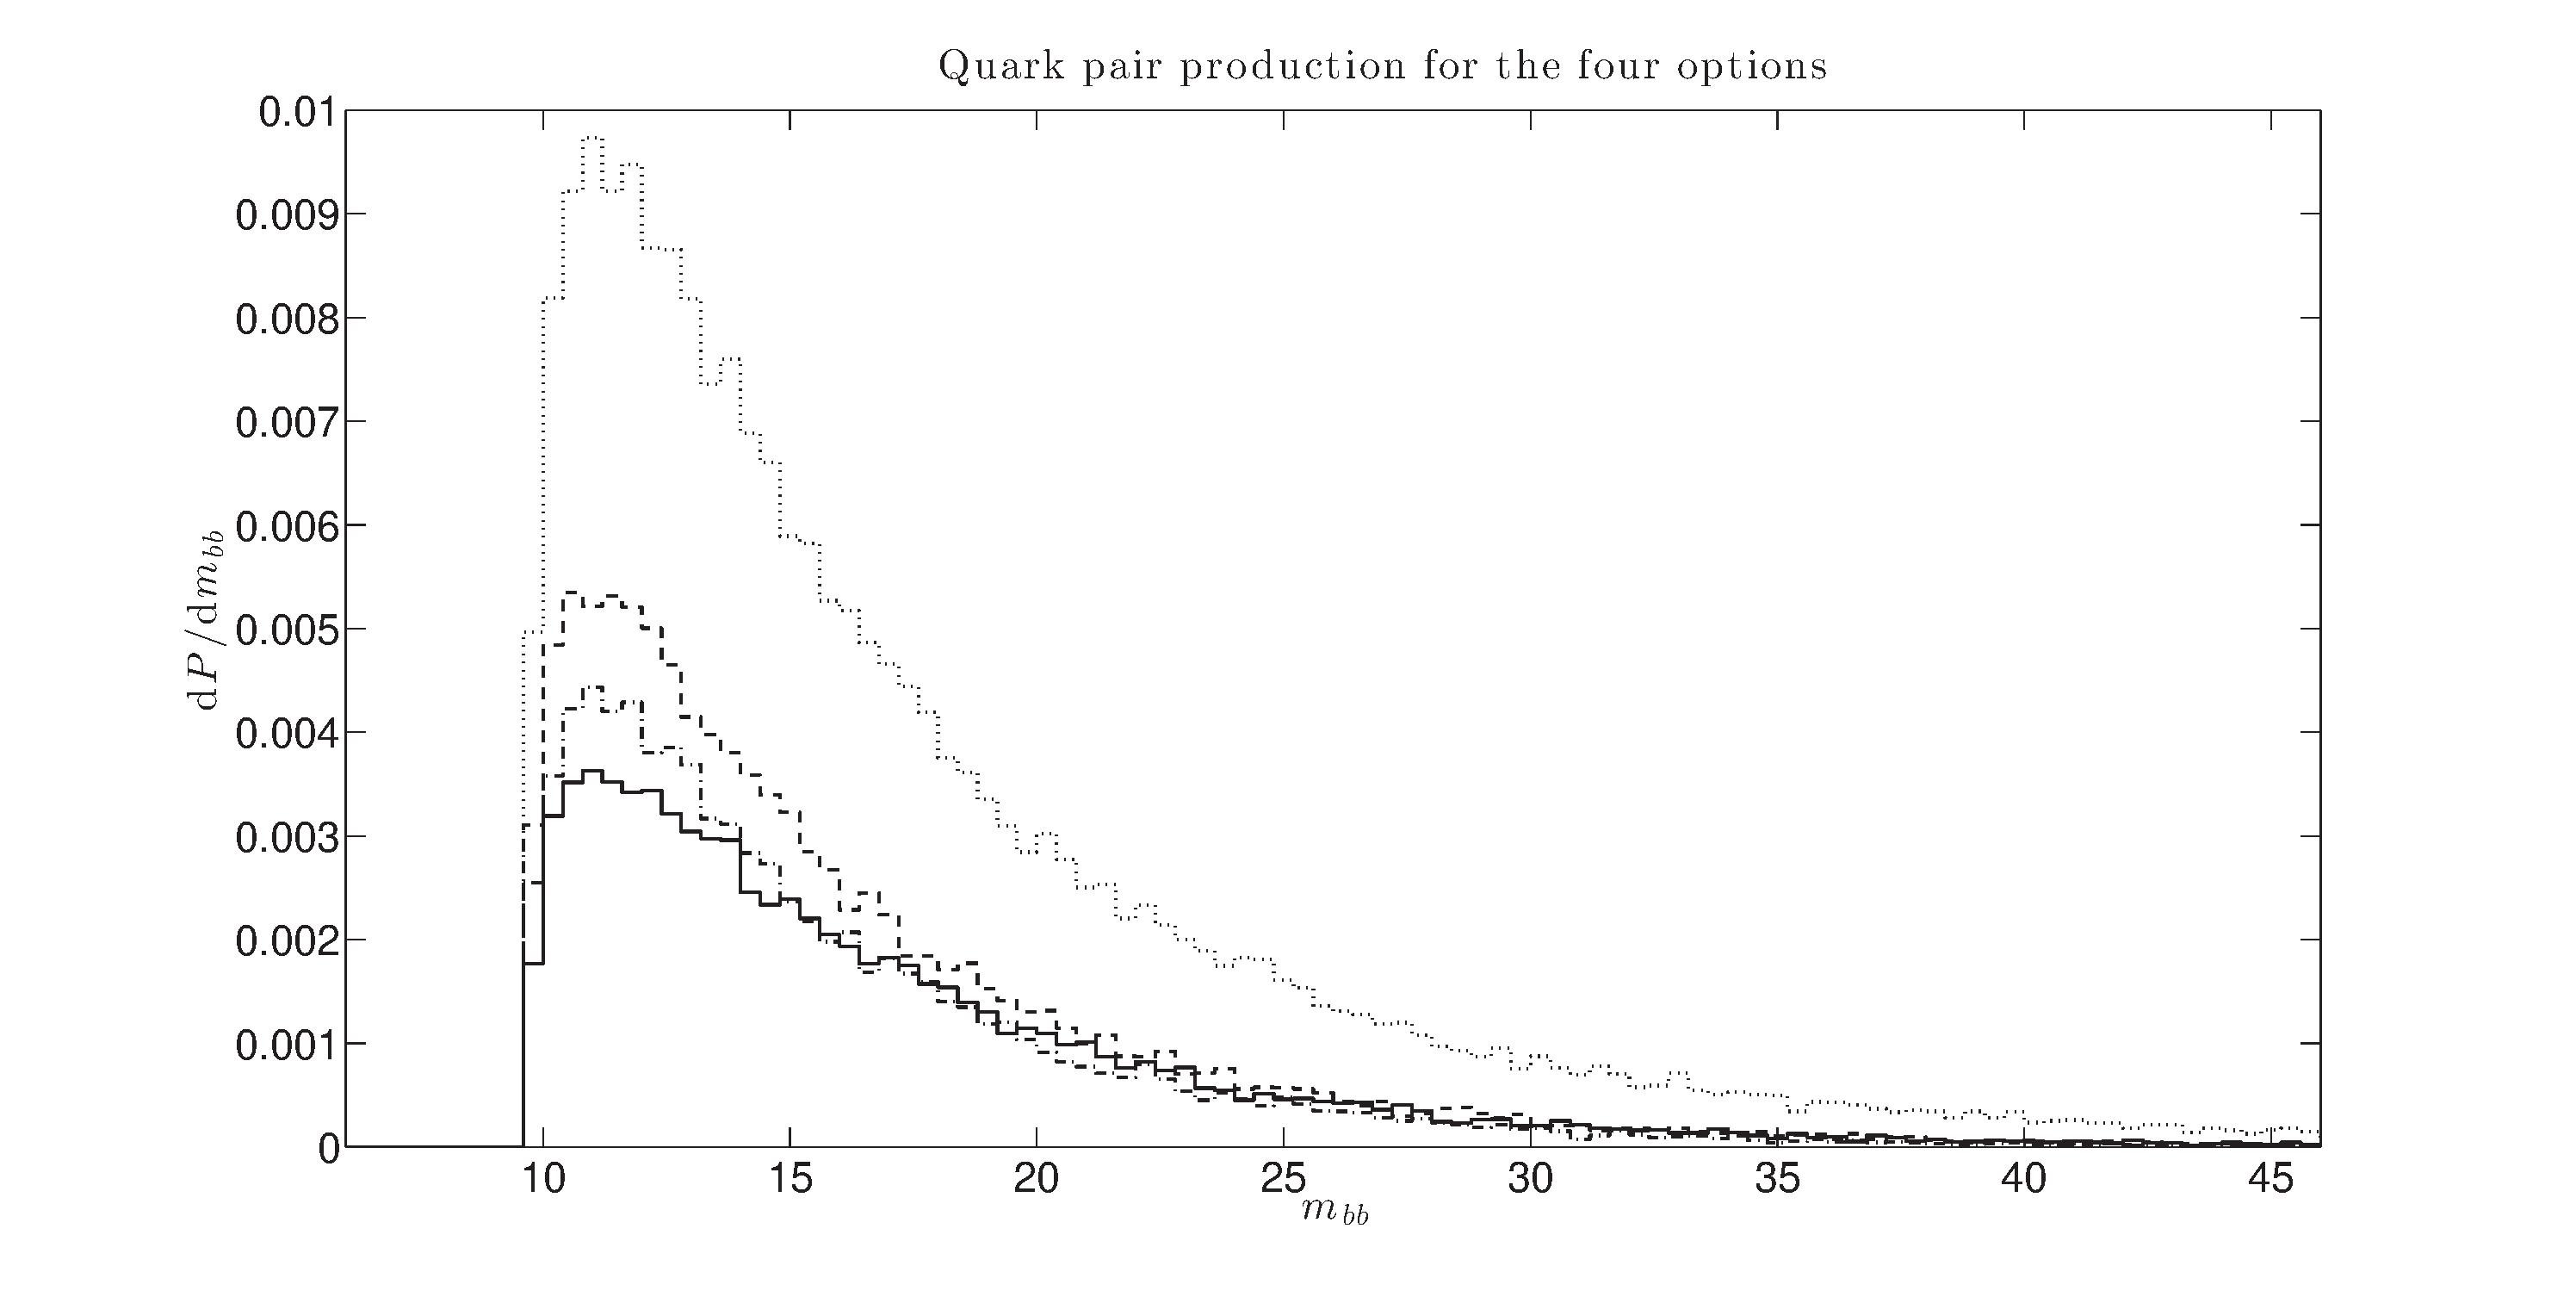
\includegraphics[width=15cm]{QMass}
\label{fig:QMass}
\end{figure}



Las características importantes de las opciones 1-4, discutidas en \ref{subsubsec:PythiaAlg}, están presentes en este gráfico. La opción 3 representa el caso extremo. La compensación entre el acrecentamiento en la zona umbral y la supresión a masas altas es visible para la opción 4. Esta compensación corrige el valor de la tasa total (área bajo la curva) a un valor similar al dado por la opción 1. En principio, no hay ninguna razón para esperar que estos dos efectos se compensaran tan cercanamente en la tasa total. La opción 2 presenta una producción visiblemente mayor que la opción 1 en la zona umbral de producción.

Las tasas dadas por las opciones que usan $m^2$ como variable de evolución (5-8) conllevan a una tasa ligeramente menor que las dadas por las primeras 4 opciones, alrededor de 5\% menos.

Los valores dados por las opciones 1, 4, 5, 6 y 8 caen dentro del error total de las últimas tres referencias en la tabla \ref{table:gbbMeasurements}. El valor dado por la opción 2 está por poco fuera de los errores, pero aún dentro de dos desviaciones estándar. Las opciones 3 y 7 no parecieran resproducir los datos experimentales, ya que se encuentran lejanamente fuera del límite superior indicado por todas las mediciones.

Las discrepancias pueden estar relacionadas a la masa desnuda del quark bottom, una cantidad que no puede ser medida directamente. Usando una masa $m_\b$ más alta que la dada por defecto, las tasas simuladas se reducirían, acercándose más a los resultados experimentales. Además, tomando en cuenta los errores sistemáticos mostrados en la tabla \ref{table:gbbMeasurements} y la dispersión de los valores, podemos notar que se trata de una medición complicada.

\subsection{El espectro de la fracción de energía de los mesones $\D^{*\pm}$}

Vamos a estudiar ahora la producción de mesones $\D^{*\pm}$ como función de la fracción de energía $X_E$. La colaboración ALEPH tiene mediciones para esto en \cite{Barate:1999bg}. El espectro total es tomado como la suma de tres componentes: mesones provenientes de charms primarios, de bottoms primarios y de quarks pesados secundarios, es decir, provenientes de ramificaciones a partir de gluones.

\begin{figure}[h]
\centering
\caption[Espectro de la fracción de energía de los mesones $\D^{*\pm}$.]{Distribución de la fracción de energía para los mesones  $\D^{*\pm}$. Los puntos con barras de error son las mediciones de ALEPH  y la línea sólida corresponde a la simulación de \textsc{Pythia}, con las contribuciones correspondientes de: $\b\bbar$ (puntos), $\c\cbar$ (líneas) y ramificaciones de gluón (líneas y puntos).}
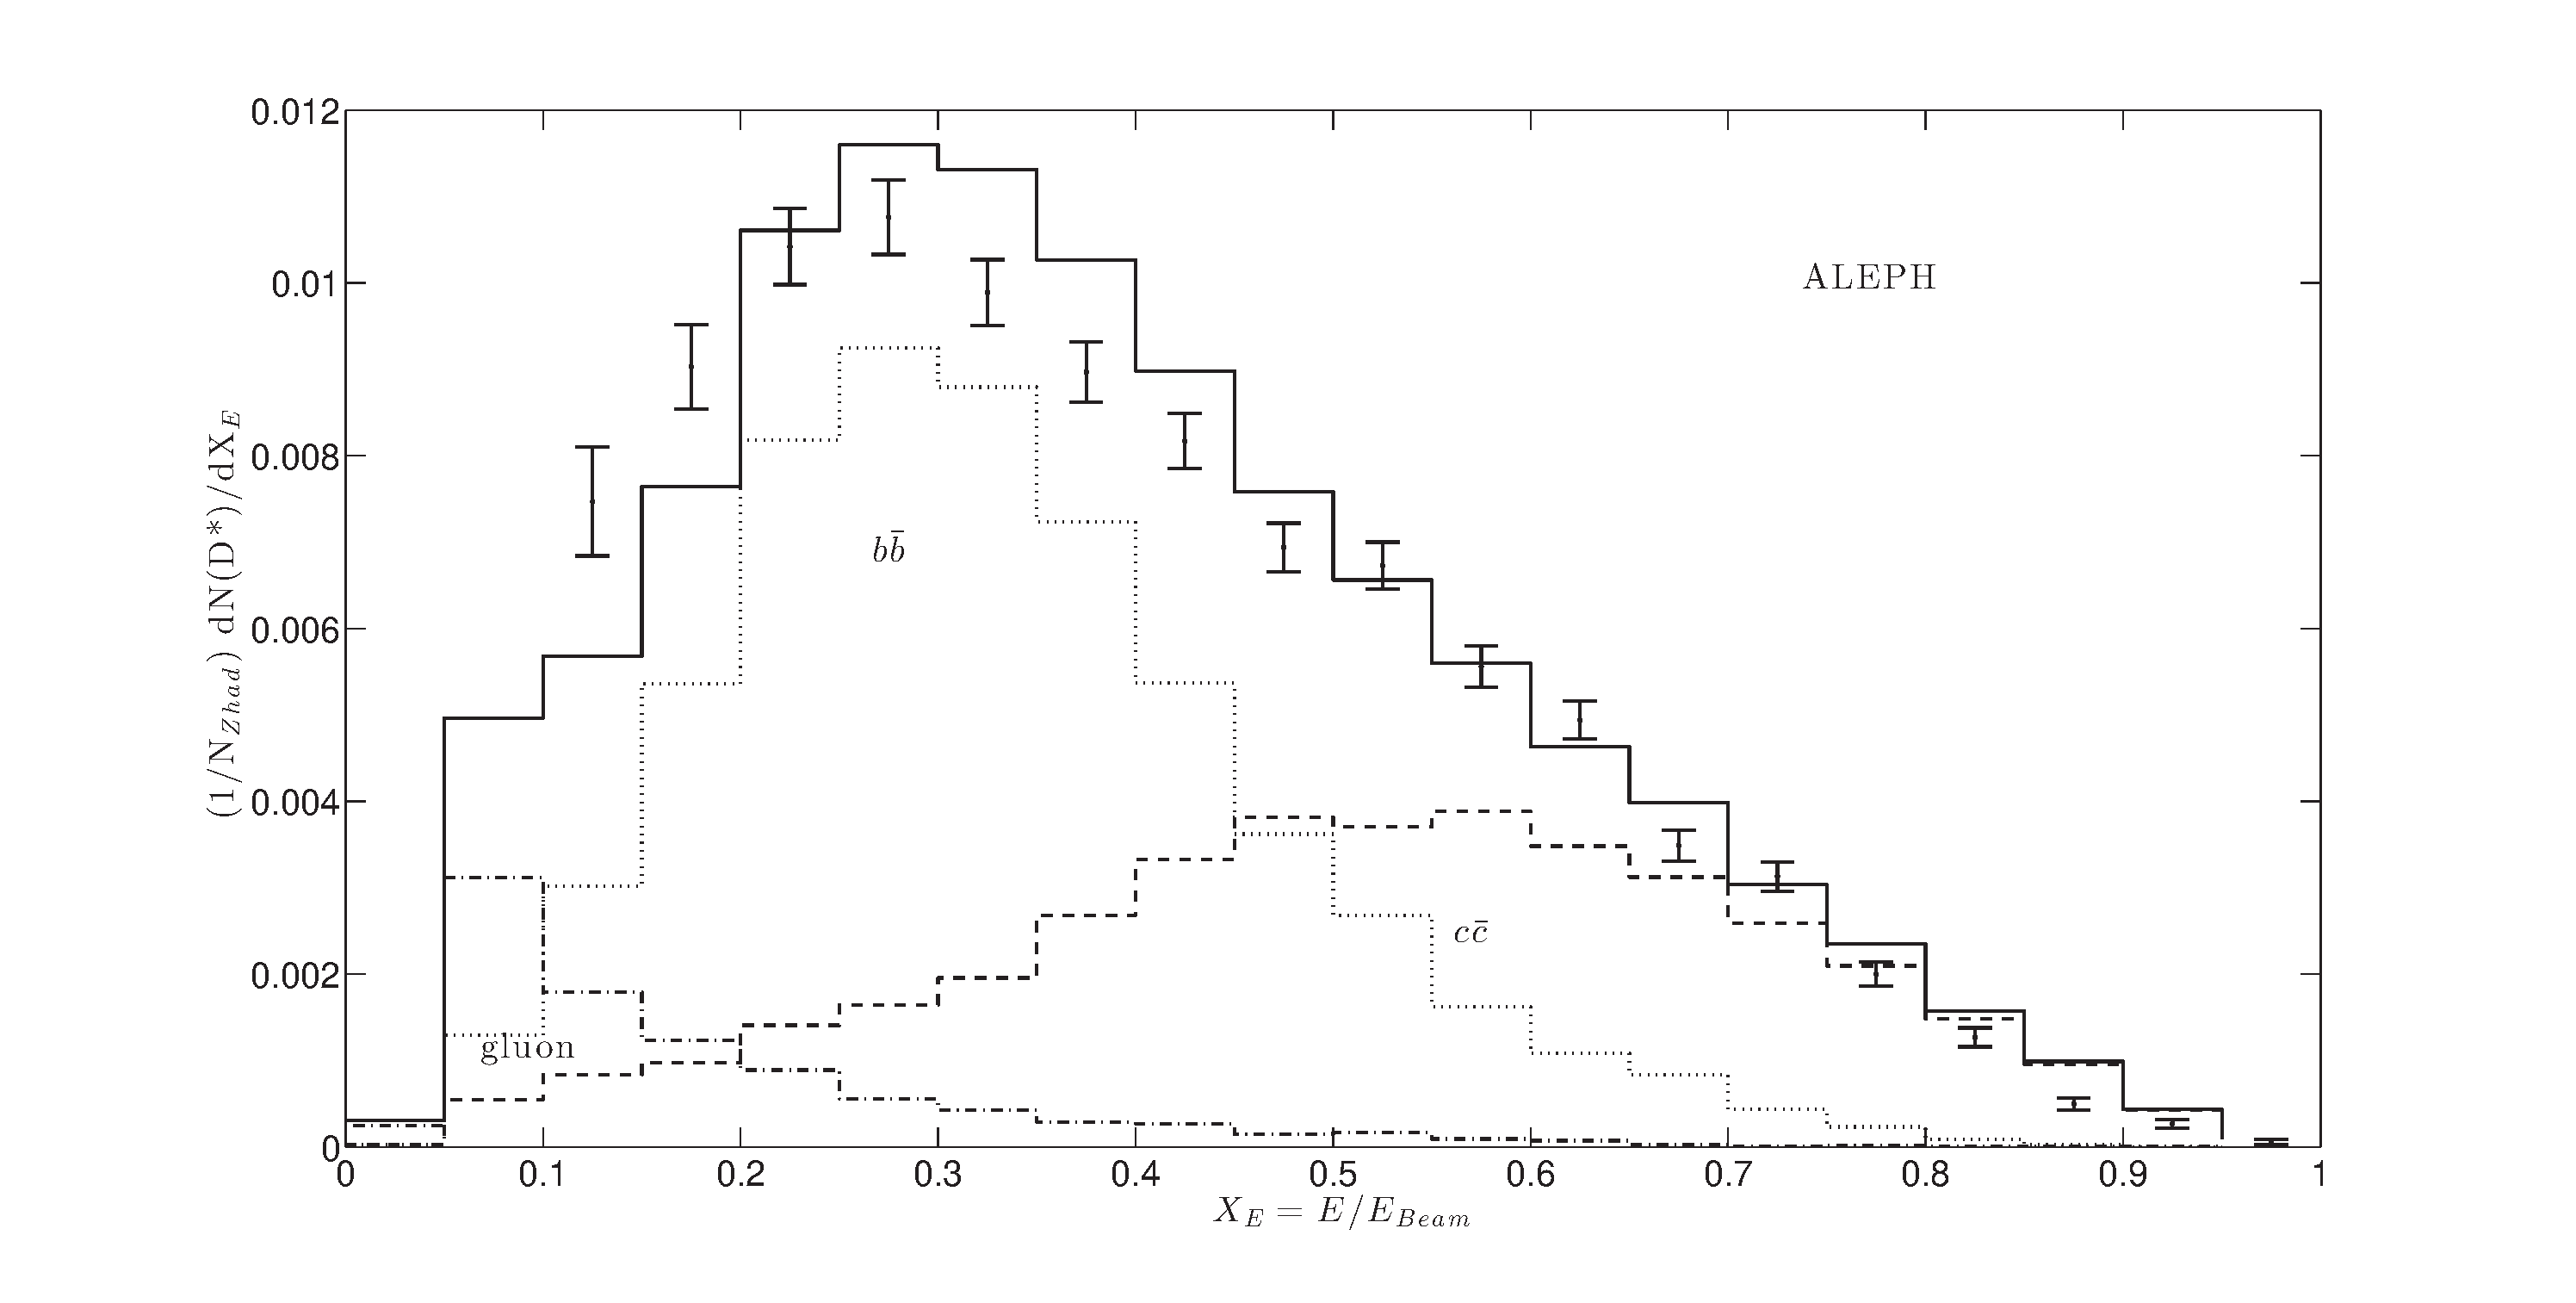
\includegraphics[width=15cm]{DStarOp1Thesis}
\label{fig:ALEPHPythia1}
\end{figure}



En gráfico en la figura \ref{fig:ALEPHPythia1} muestra que las mediciones de ALEPH y la simulación de \textsc{Pythia} (opción 1) con sus componentes. Podemos ver que la contribución principal de la ramificación de gluones sucede a fracciones de energía bajas, lo que se debe al hecho de que los quarks secundarios son producidos al menos en una tercera ramificación, partiendo desde el $Z^0$ (como en la figura \ref{fig:PrimSecQuarks}), cuando ya la energía ha sido distribuída en varios productos. De este modo, el impacto de las opciones será a fracciones de energía bajas. La figura también sugiere la necesidad de una corrección a energías bajas, incluso para las contribuciones de $\b\bbar$ y $\c\cbar$ primarios. Además, la simulación presenta un exceso justo después del pico cercano a $0.3$. Para valores medianos y altos de $X_E$, la simulación y los experimentos concuerdan en buena medida.

La figura \ref{fig:GluonDStar} muestra los casos extremos para la contribución de gluones: opciones 1 y 3. La última presenta valores al menos dos veces mayores que la primera en cada casilla del histograma. Las distribuciones para las opciones 2 y 4 (que no se muestran) dan valores intermedios.

\begin{figure}[h]
\centering
\caption[Contribución de los gluones a la producción de $\D^{*\pm}$ en dos casos extremos.]{Casos extremos de la producción de $\D^{*}$ a partir de gluones. Opciones de \textsc{Pythia} 1 (sólida) y 3 (punteada).}
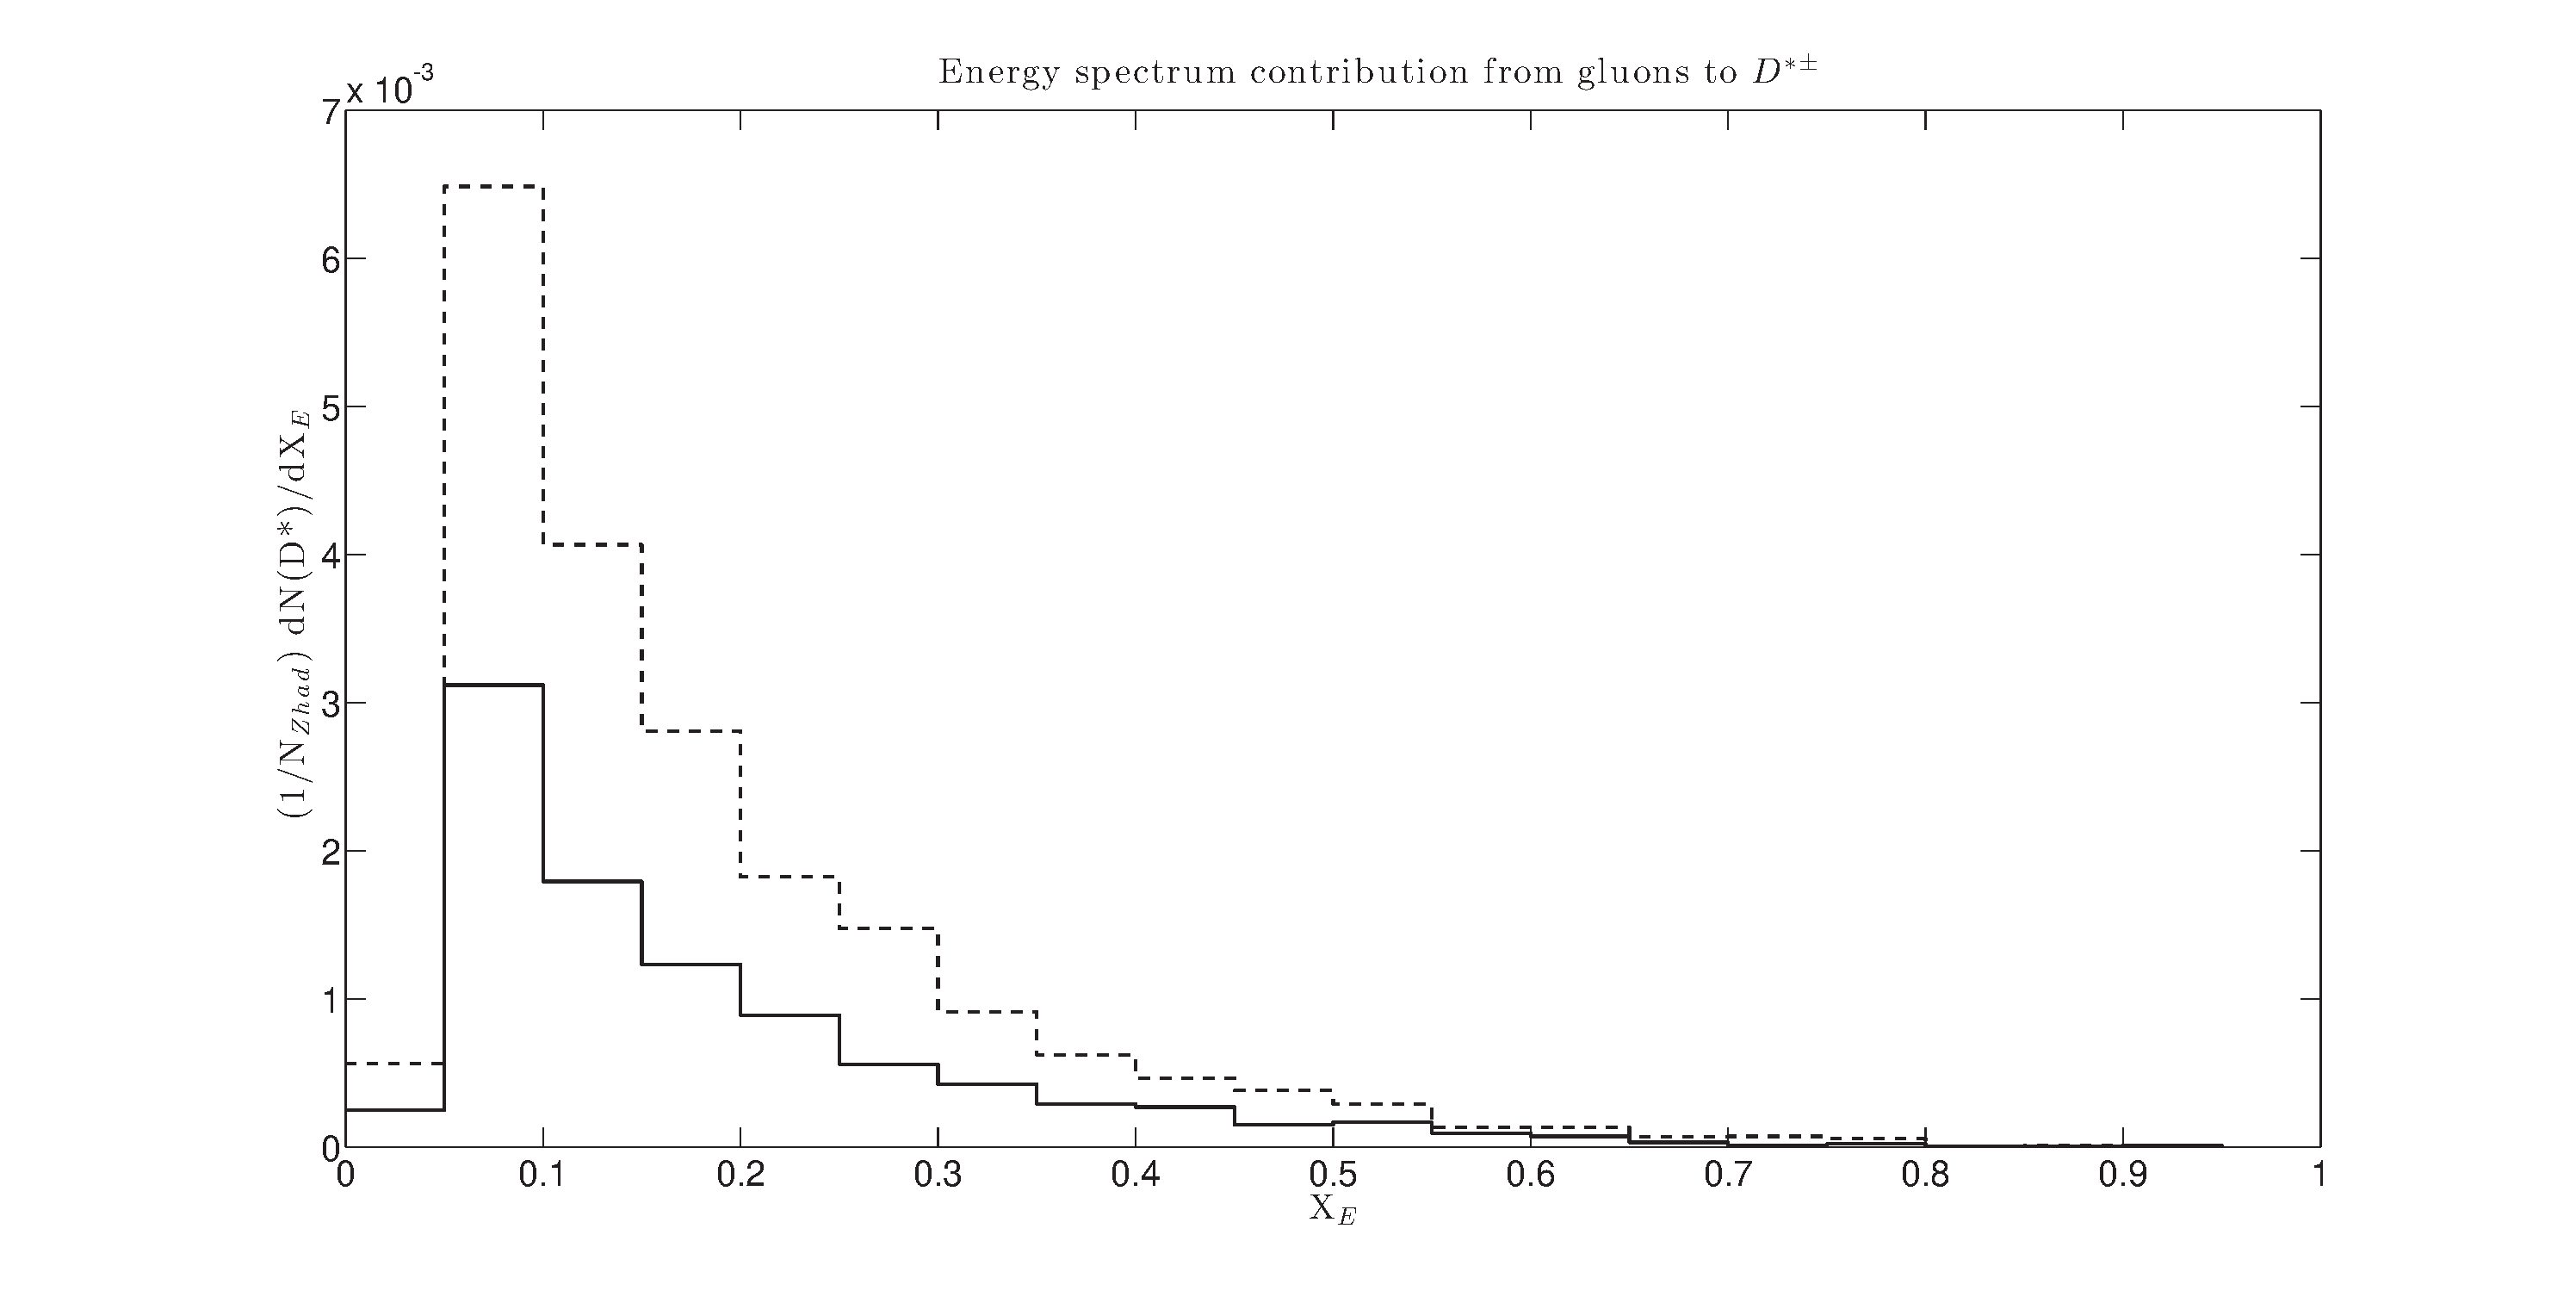
\includegraphics[width=15cm]{GluonDStarThesis}
\label{fig:GluonDStar}
\end{figure}

Para comparar las cuatro opciones con los datos experimentales, la figura \ref{fig:DStarOp} muestra las distribuciones completas y las mediciones de ALEPH. El aumento de producción a bajas energías es evidente para las opciones que no son por defecto, donde las simulaciones se acercan más a los valores experimentales. El exceso cercano al pico está todavía presente y ligeramente aumentado. A altas energías, el decaimiento no muestra diferencias significativas con respecto a la opción por defecto (debido a que en esta zona la contribución secundaria es despreciable) y siguen aproximadamente el comportamiento de los datos.

\begin{figure}[!h]
\centering
\caption[Espectro de la fracción de energía de $\D^{*\pm}$. Simulación y datos comparados.]{Espectro de la fracción de energía de $\D^{*\pm}$. Datos de ALEPH (puntos con barras de error) y las opciones de \textsc{Pythia}: por defecto (sólida), 2 (puntos), 3 (líneas) y 4 (líneas y puntos).}
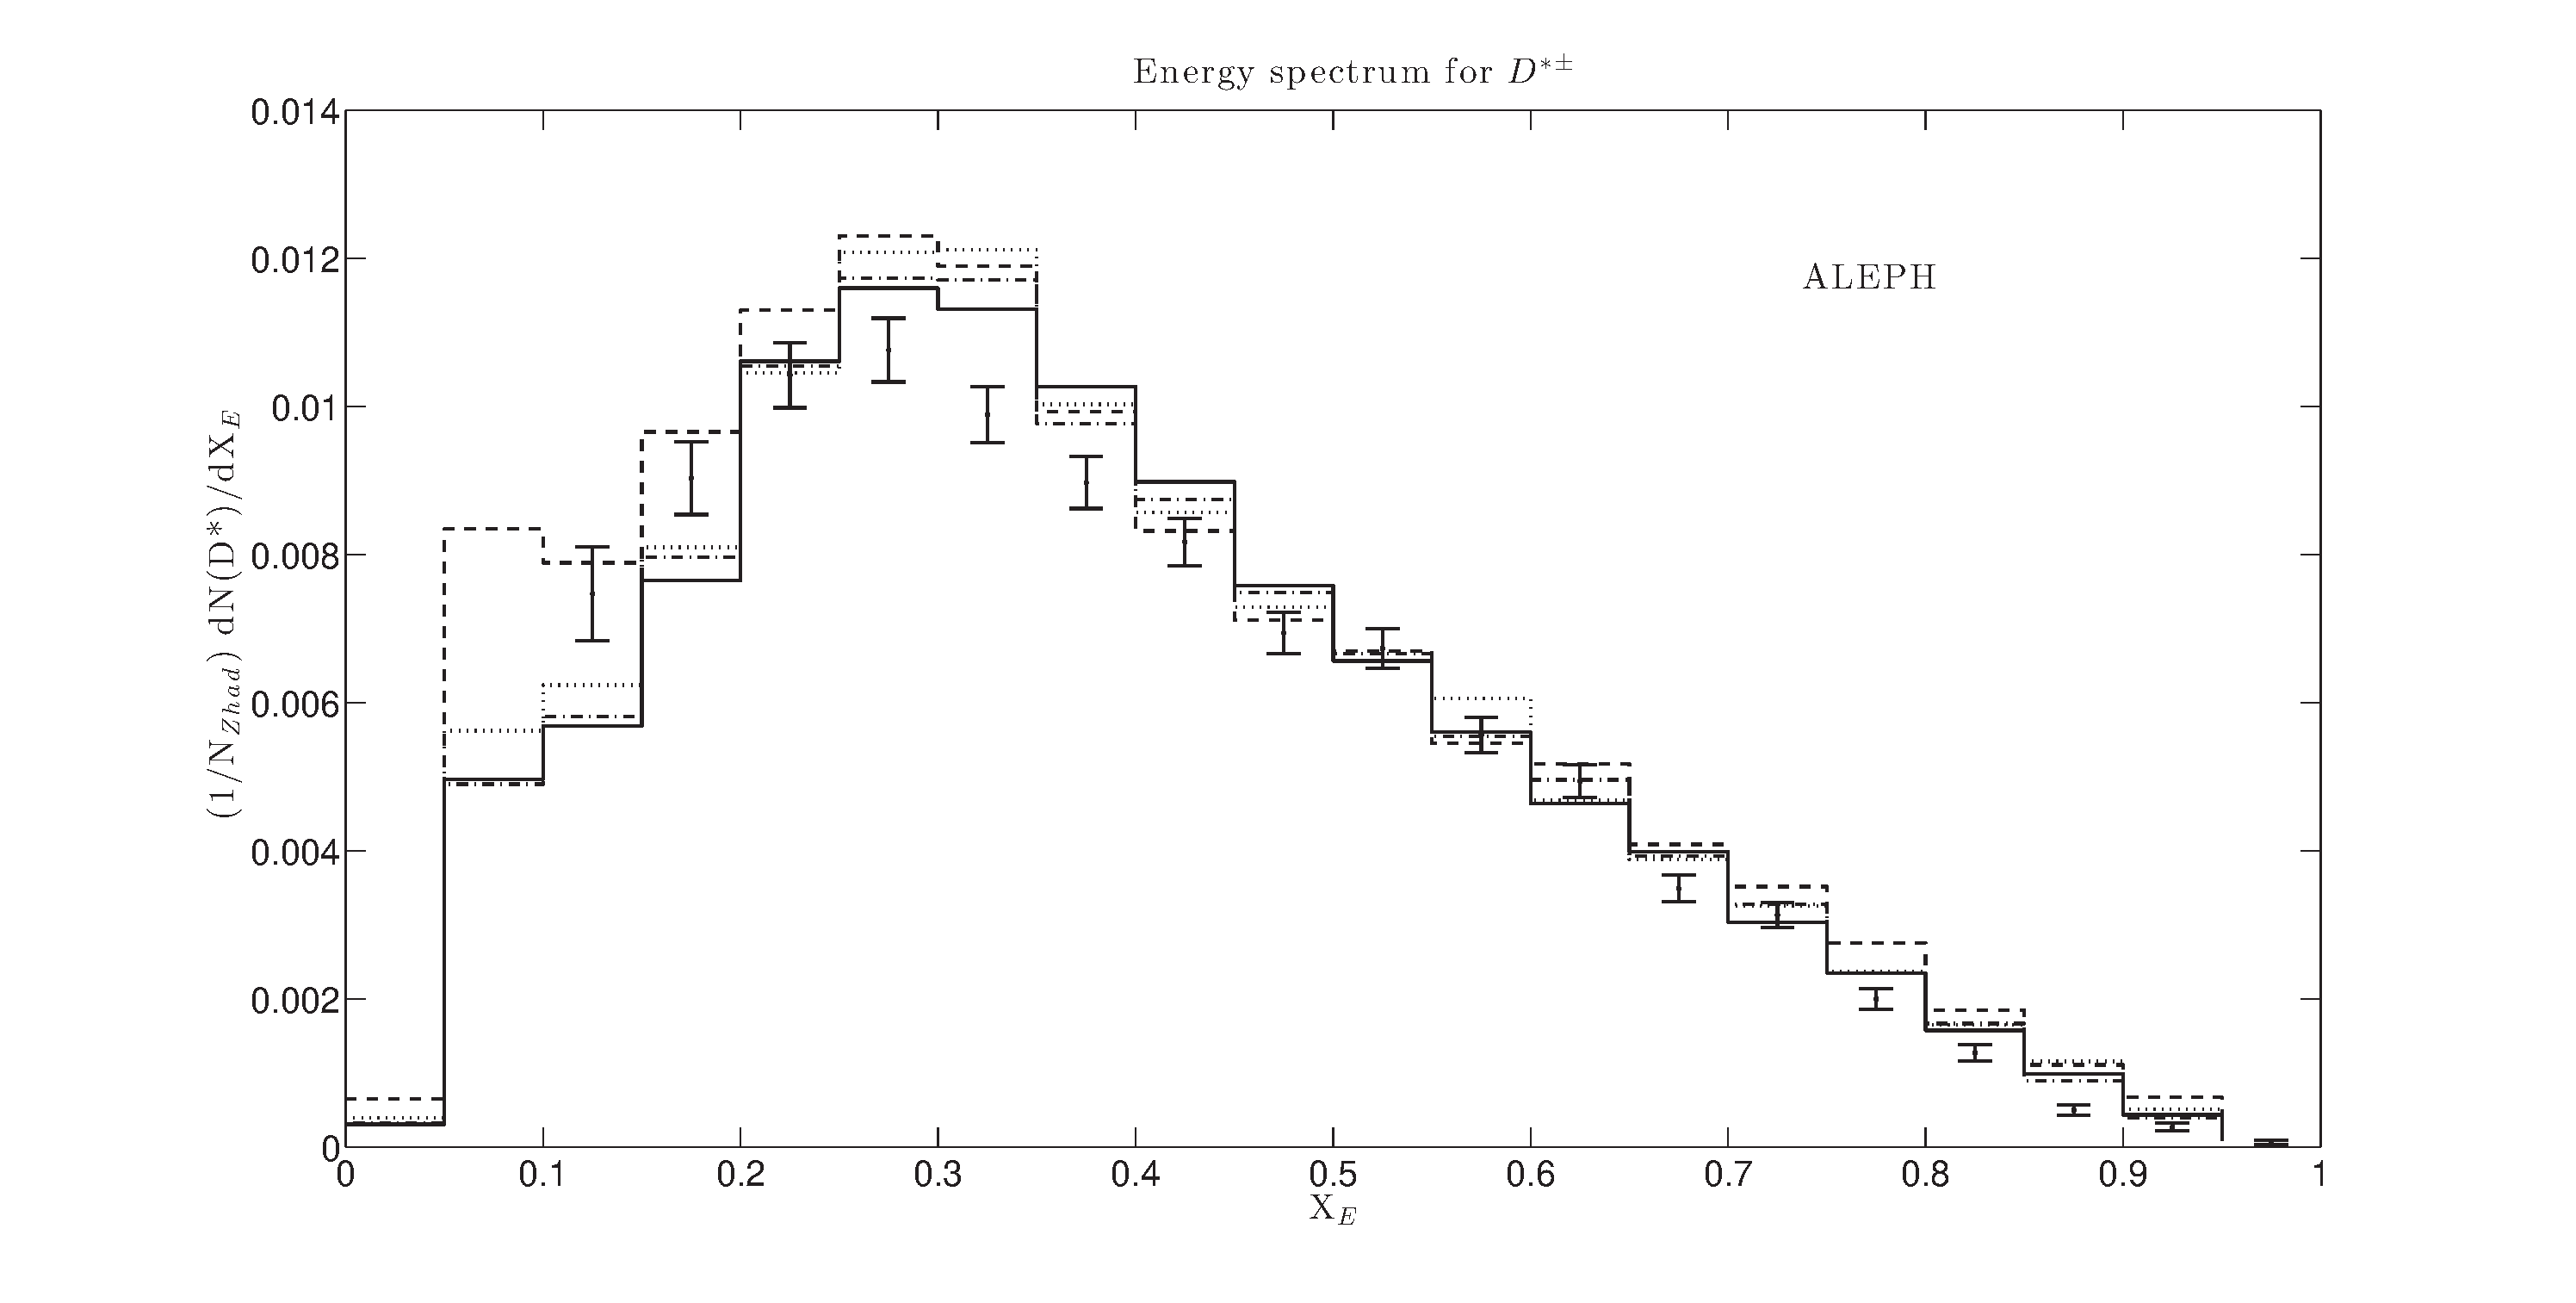
\includegraphics[width=15cm]{DStarOpThesis}
\label{fig:DStarOp}
\end{figure}

En este contexto, la opción 3 parece un buen candidato, debido a que corrige (con algo de precisión) la producción de mesones $\D^*$ a bajas energías. Para la región justo después del pico, el aumento puede ser mayor al deseado, pero aún así los datos en su totalidad son más cercanos a esta opción.

Debido a su carácter no-perturbativo, el decaimiento de mesones es un fenómeno que no se entiende completamente. Un modelado algo diferente del decaimiento $\B\to D$ pudiera correr algunos eventos después del pico a más bajas energías, para ajustarse mejor a los datos experimentales en ambas regiones, sin requerir una tasa $\g\to\b\bbar$ mayor. De esta manera, este estudio no puede concluir definitivamente sobre esta desviación.

\section{Colisiones protón-protón a 7000 GeV}

Tornando ahora al tema de las colisiones hadrónicas, estudiaremos las correlaciones entre pares de hadrones $\B$. Eventos con un par son clasificados de acuerdo a PC, FE y GS. Eventos con más pares son clasificados como mezclados.

Una simulación de $5\times10^6$ eventos fue llevada a cabo para cada opción. Fueron seleccionados para el análisis eventos con dos mesones $\B$, cada uno con un momentum transverso mayor a 15 GeV. Un corte inferior para el momentum transverso del proceso duro de 15 GeV también fue impuesto; este criterio es necesario debido a que eventos con $\pT$ más bajo son producidos en mayor cantidad, pero el número de eventos seleccionados decrece para valores menores de 20 GeV, como se puede ver en la figura \ref{fig:accepted}. Allí, sólo alrededor del 1\% de los eventos son seleccionados para el análisis. Un corte aún más bajo incrementaría tal ``ineficiencia'', seleccionando sólo unos pocos más eventos en comparación con el total generado.

\begin{figure}[h]
\centering
\caption[Eventos generados y aceptados en colisiones hadrónicas.]{Eventos generados (sólida) y aceptados (punteada) como función del momentum transverso del proceso.}
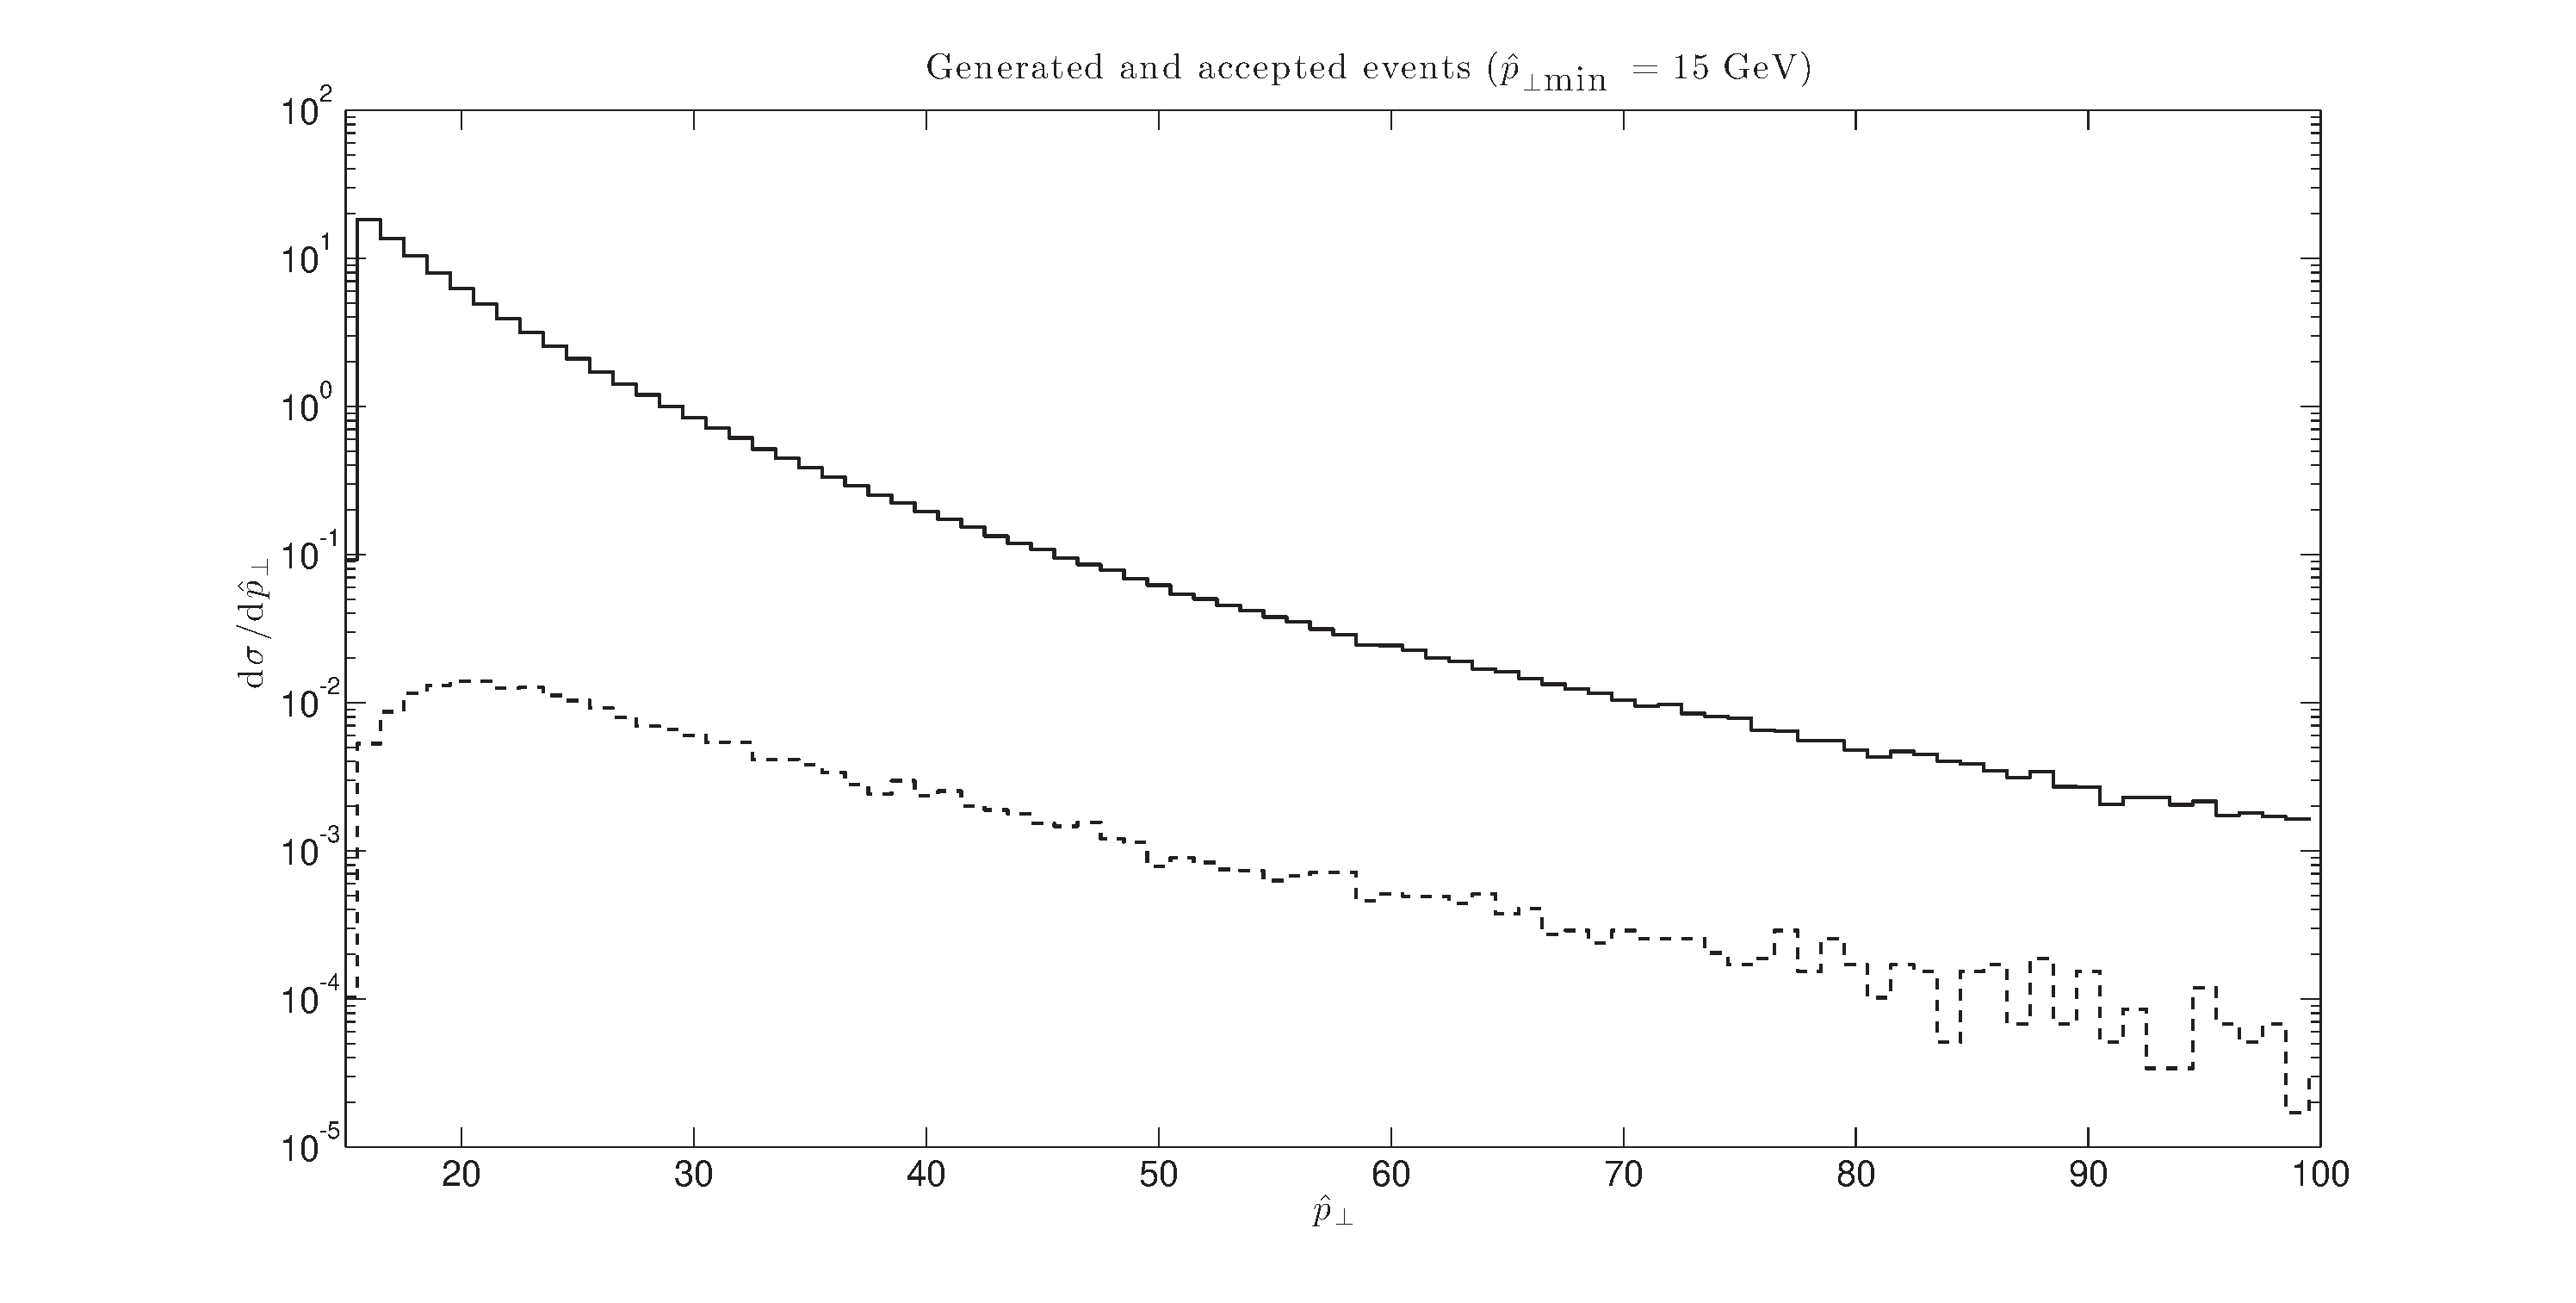
\includegraphics[width=15cm]{Accepted}
\label{fig:accepted}
\end{figure}

\subsection{Separaciones azimutales angulares}

La variación del ángulo azimutal es una buena medida de la separación de dos mesones $\B$, debido a que es un invariante de Lorentz bajo boosts a lo largo del eje de colisión ($z$). La diferencia $\Delta \varphi$  es medida en el plano perpendicular al eje $z$. La figura \ref{fig:BBPhiOp1}  muestra la producción de pares de mesones bottom en términos de la separación angular azimutal, para la opción 1.

\begin{figure}[!h]
\centering
\caption[Separación angular azimutal de pares de mesones $\B$. Opción por defecto de \textsc{Pythia}.]{Separación angular azimutal de pares de mesones $\B$ usando la opción por defecto de \textsc{Pythia} incluyendo las cuatro fuentes de producción.}
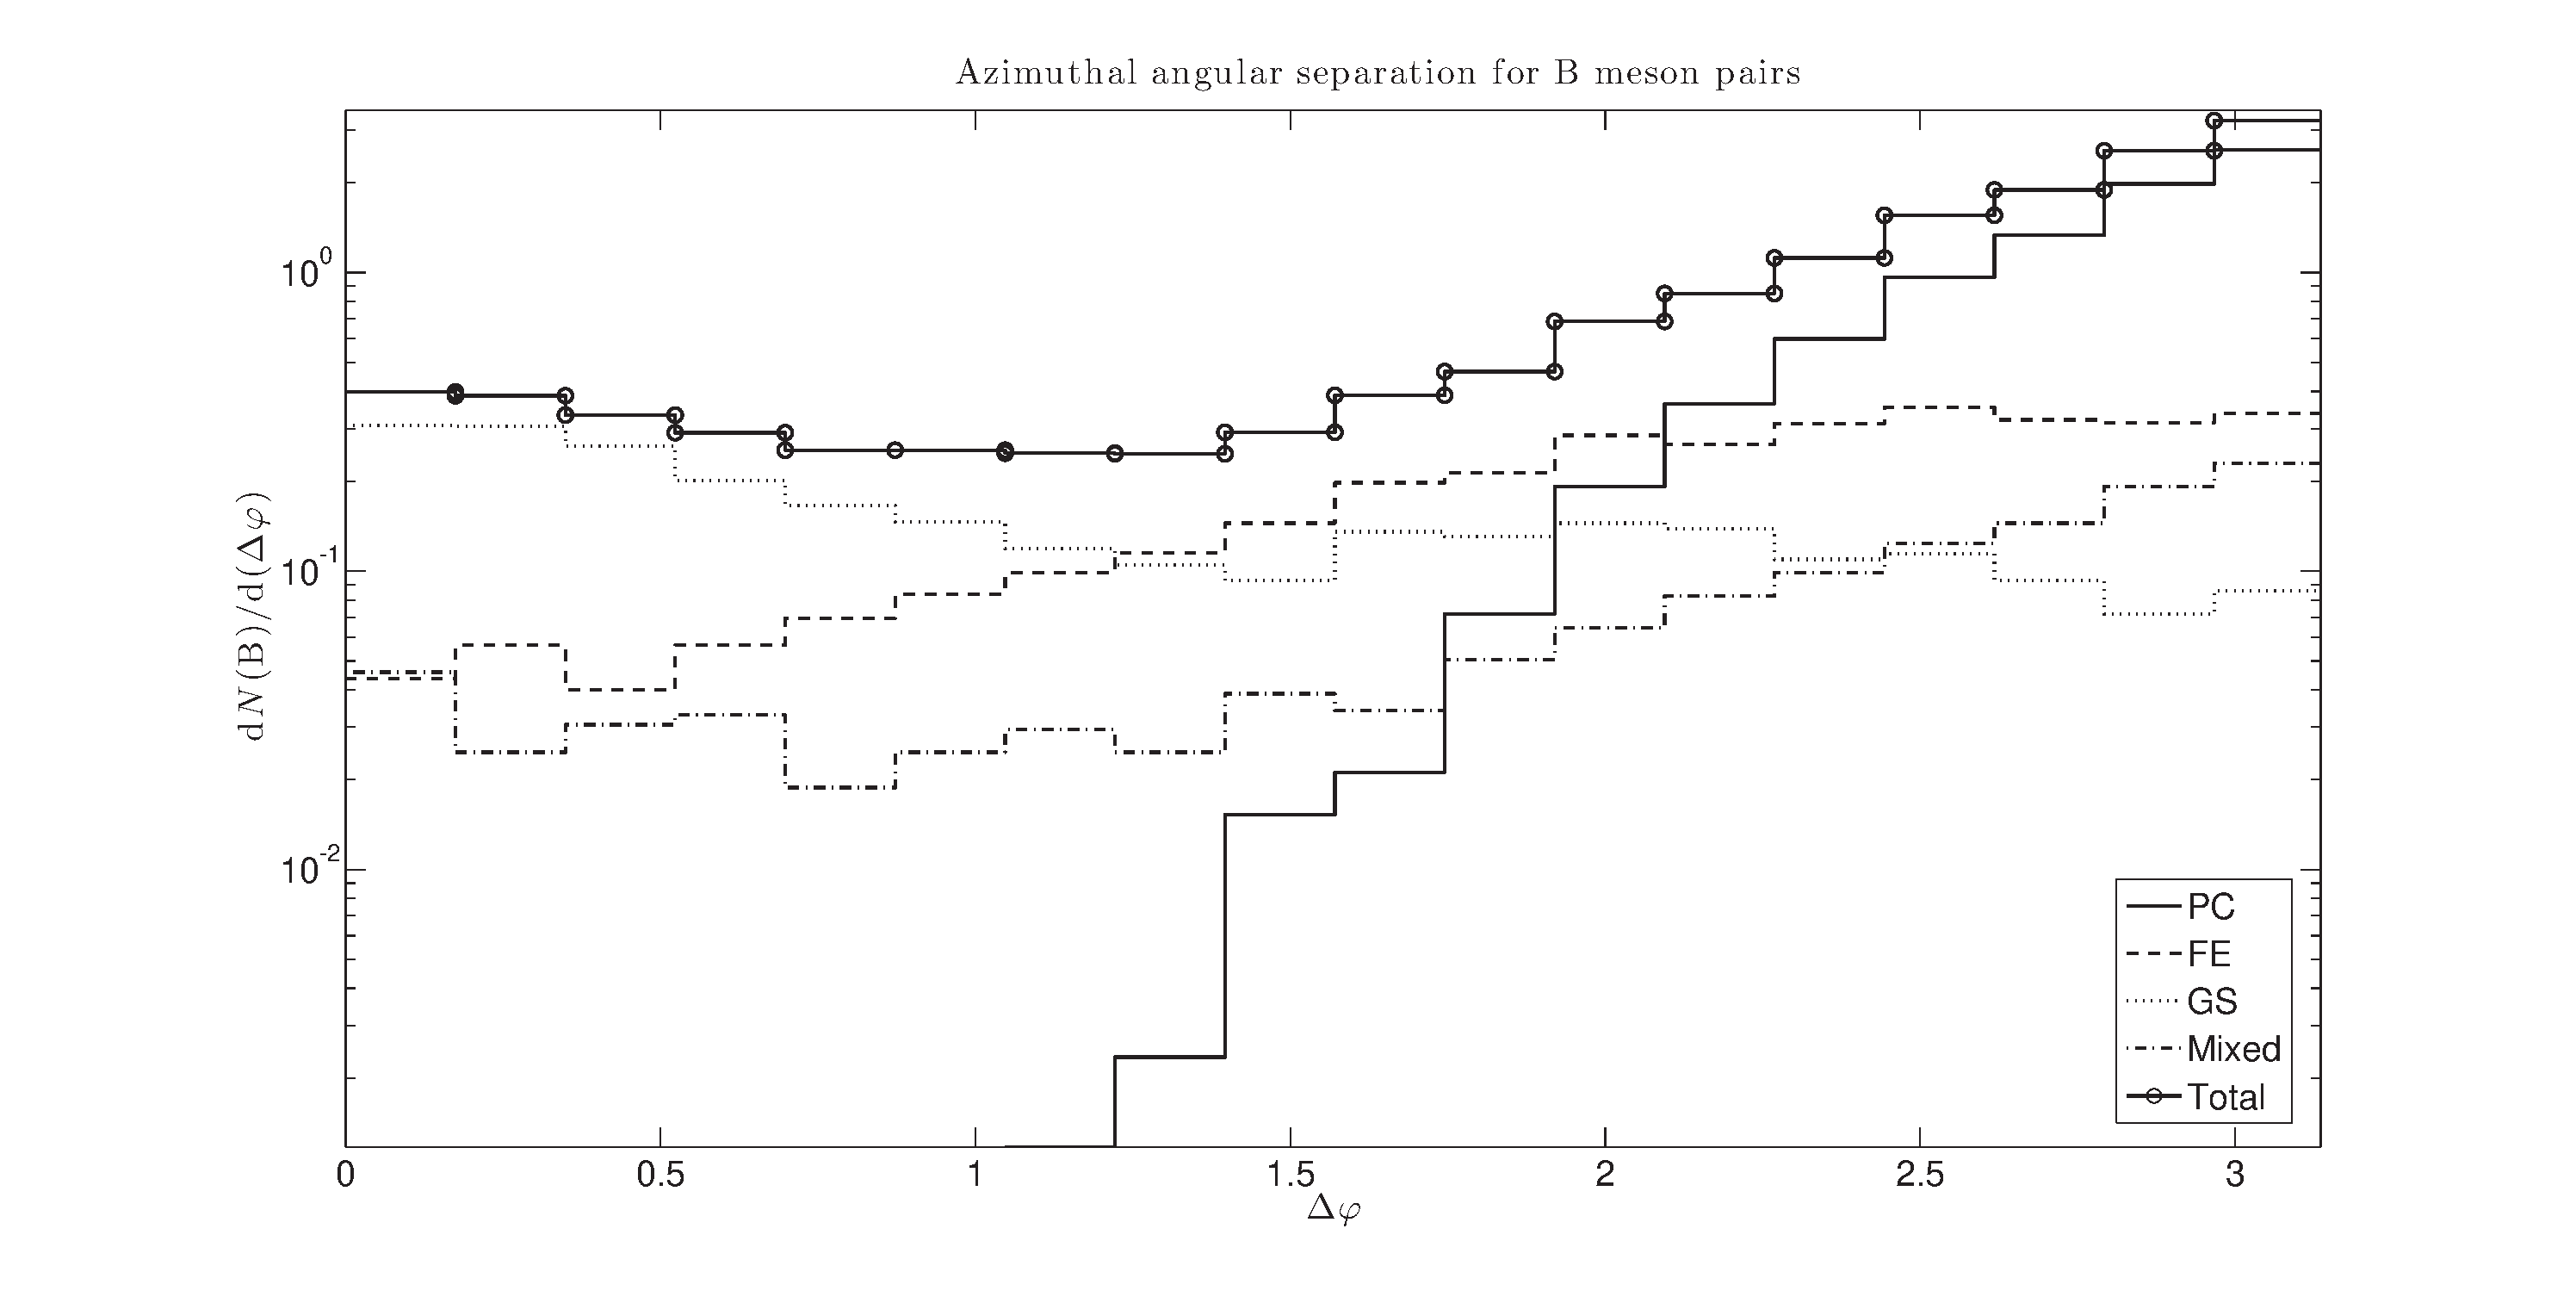
\includegraphics[width=15cm]{BBPhiOp1}
\label{fig:BBPhiOp1}
\end{figure}
Varios rasgos de las correlaciones en los mecanismos de producción son visibles: PC muestra un pico a ángulos altos, debido a que los pares son creados en el proceso duro y tienden a producir quarks en sentidos opuestos, mientras que GS contribuye mayormente en la región de poca abertura. Pares creados a partir de FE están menos anticorrelacionados que los provenientes de PC. Los mesones $\B$ mezclados muestran una distribución angular homogénea, ya que no hay una relación particular entre los mesones provenientes de ramificaciones de gluones distintas.

La variación de las opciones de \textsc{Pythia} es mostrada en la figura \ref{fig:BBPhi4Op}.

\begin{figure}[!h]
\centering
\caption[Separación angular de pares de mesones $\B$. Cuatro opciones de \textsc{Pythia}.]{Separación angular azimutal de pares de mesones $\B$ usando las opciones de \textsc{Pythia} 1 (sólida), 2 (líneas), 3 (puntos) y 4 (líneas y puntos).}
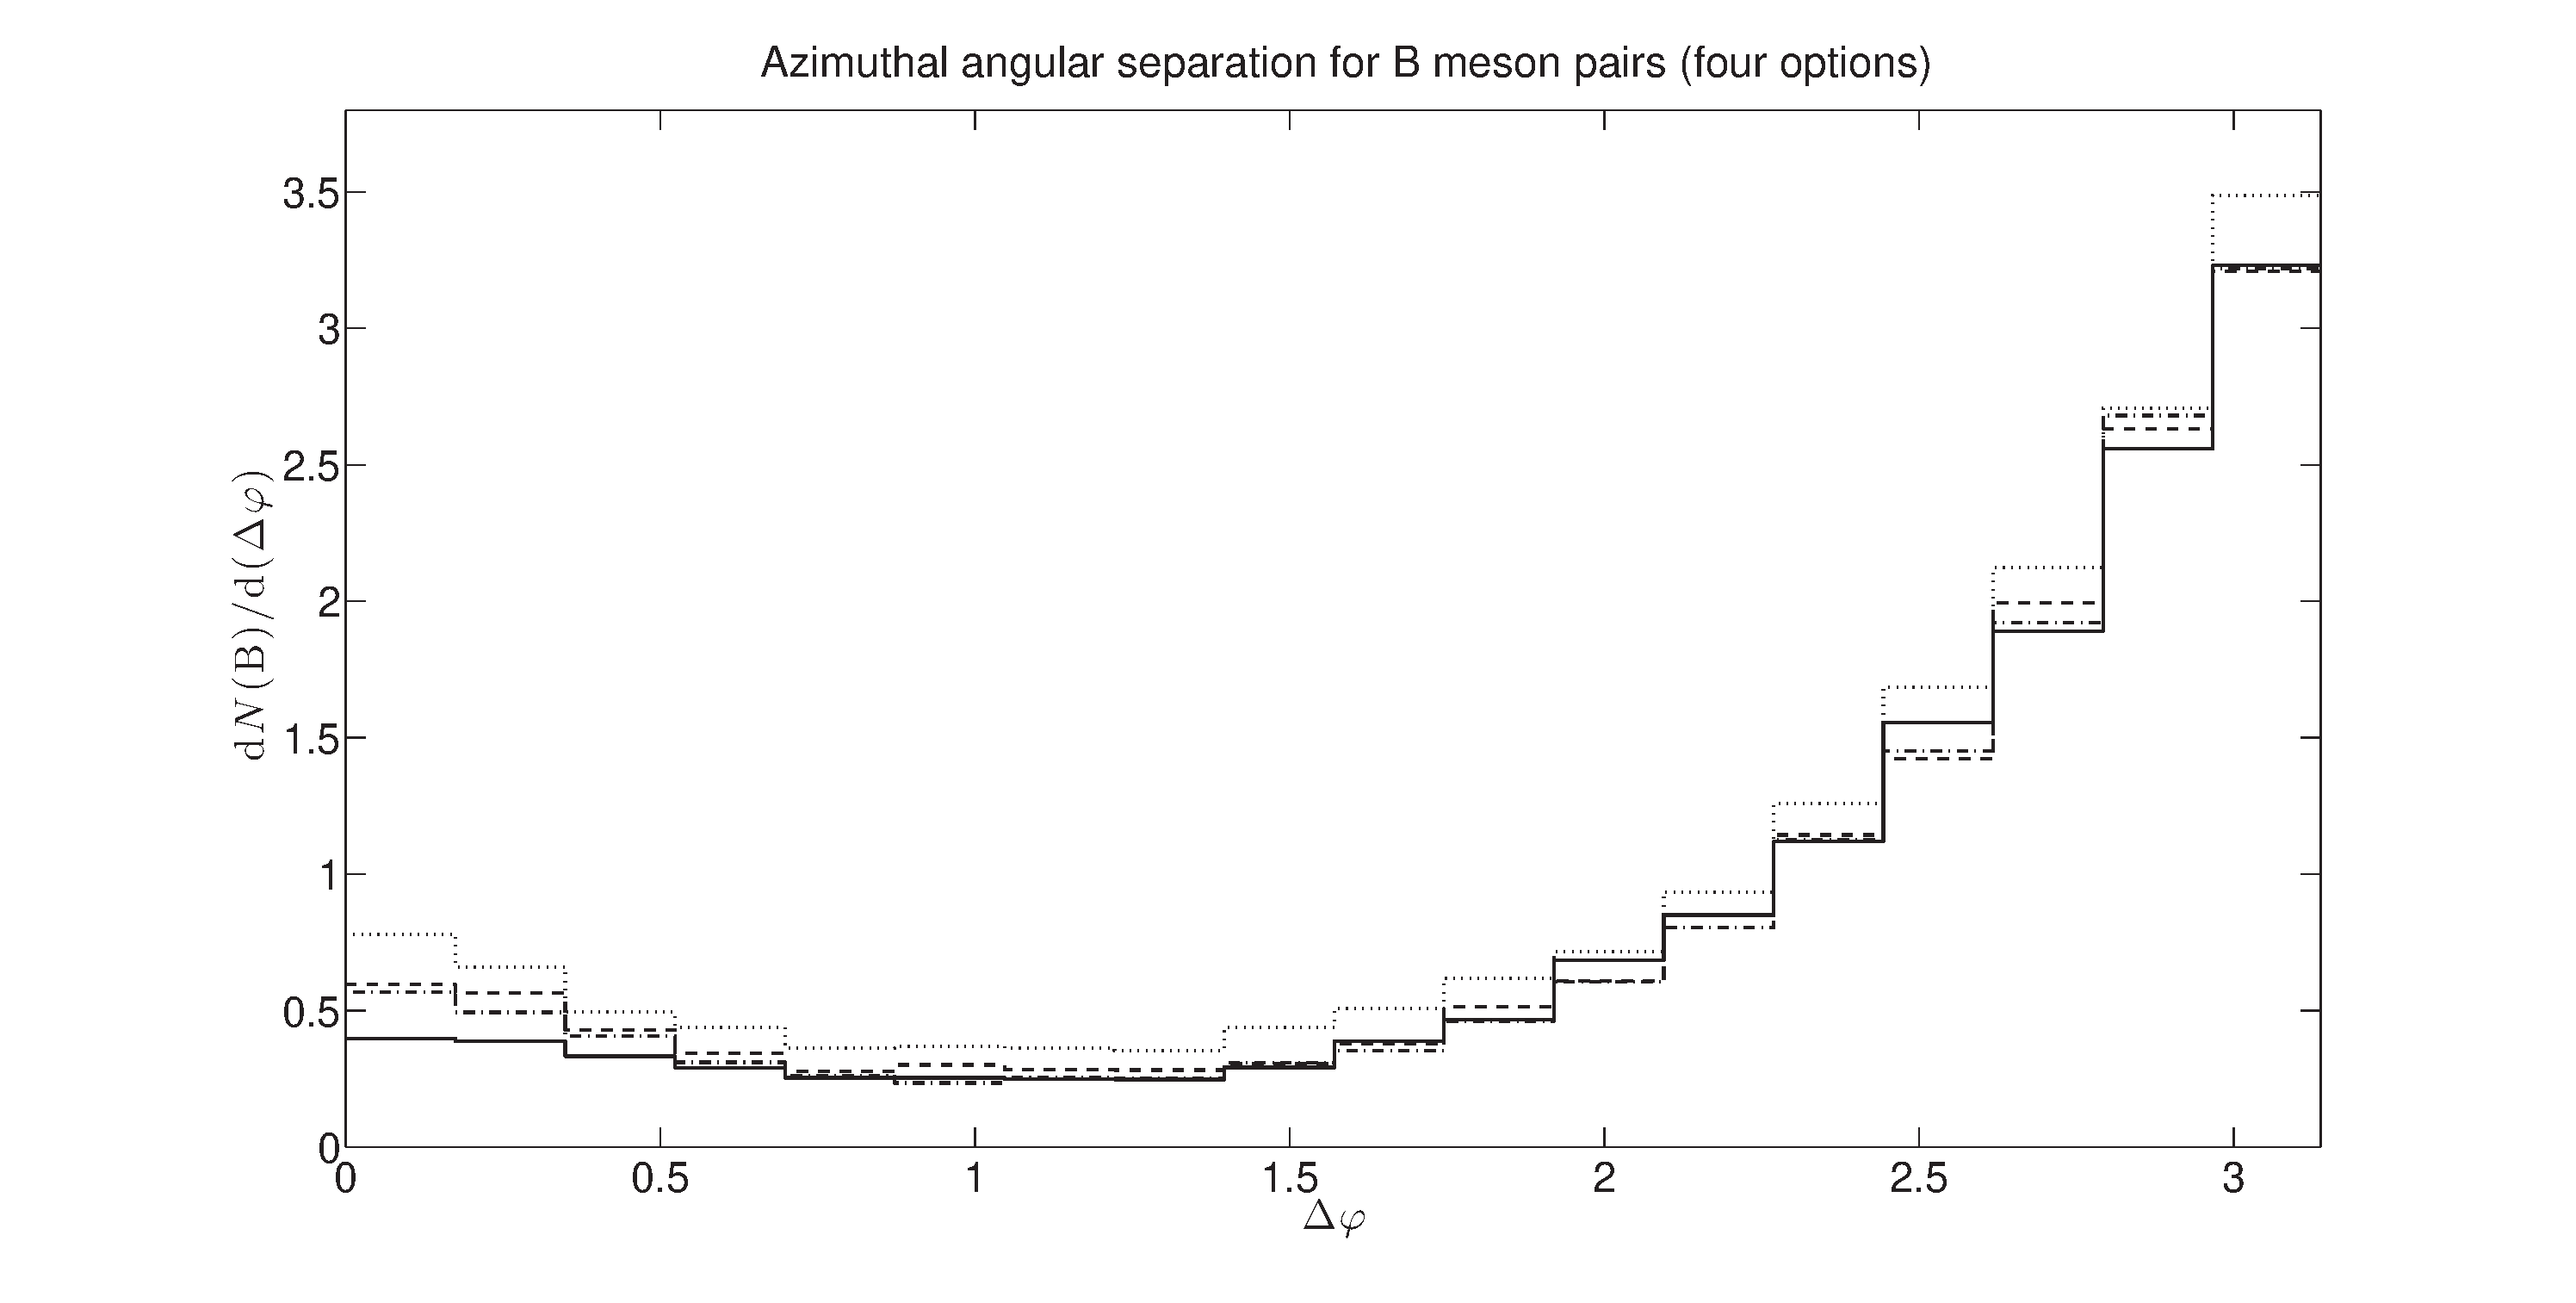
\includegraphics[width=15cm]{BBPhi4Op}
\label{fig:BBPhi4Op}
\end{figure}
De manera similar al caso discutido en la sección previa, los dos casos extremos (superior e inferior) a ángulos azimutales bajos están dados por la opciones 3 y 1, donde la ramificación de gluones es dominante. Las opciones 2 y 4 son intermedias en esta región.

\subsection{Rapideces relativas}

La rapidez, definida como

$$
y =\frac12 \ln \frac{E+p_z}{E-p_z},
$$
es una medida de la separación de la partícula al eje $z$. De hecho, está relacionada al ángulo polar (entre la partícula y el eje $z$). Se puede mostrar que la diferencia $\Delta y \equiv y_2 - y_1$ es invariante bajo un boost a lo largo del eje $z$.

En gráfico en la figura \ref{fig:BBYOp1} muestra la producción de pares de mesones $\B$ como una función de las rapideces relativas $\Delta y$, simuladas con la opción por defecto de \textsc{Pythia}.

\begin{figure}[!h]
\centering
\caption[Rapidez relativa de pares de mesones $\B$. Opción por defecto de \textsc{Pythia}.]{Rapidez relatica de pares de mesones $\B$ usando la opción por defecto de \textsc{Pythia}, incluyendo la clasificaciónd e las fuentes de producción.}
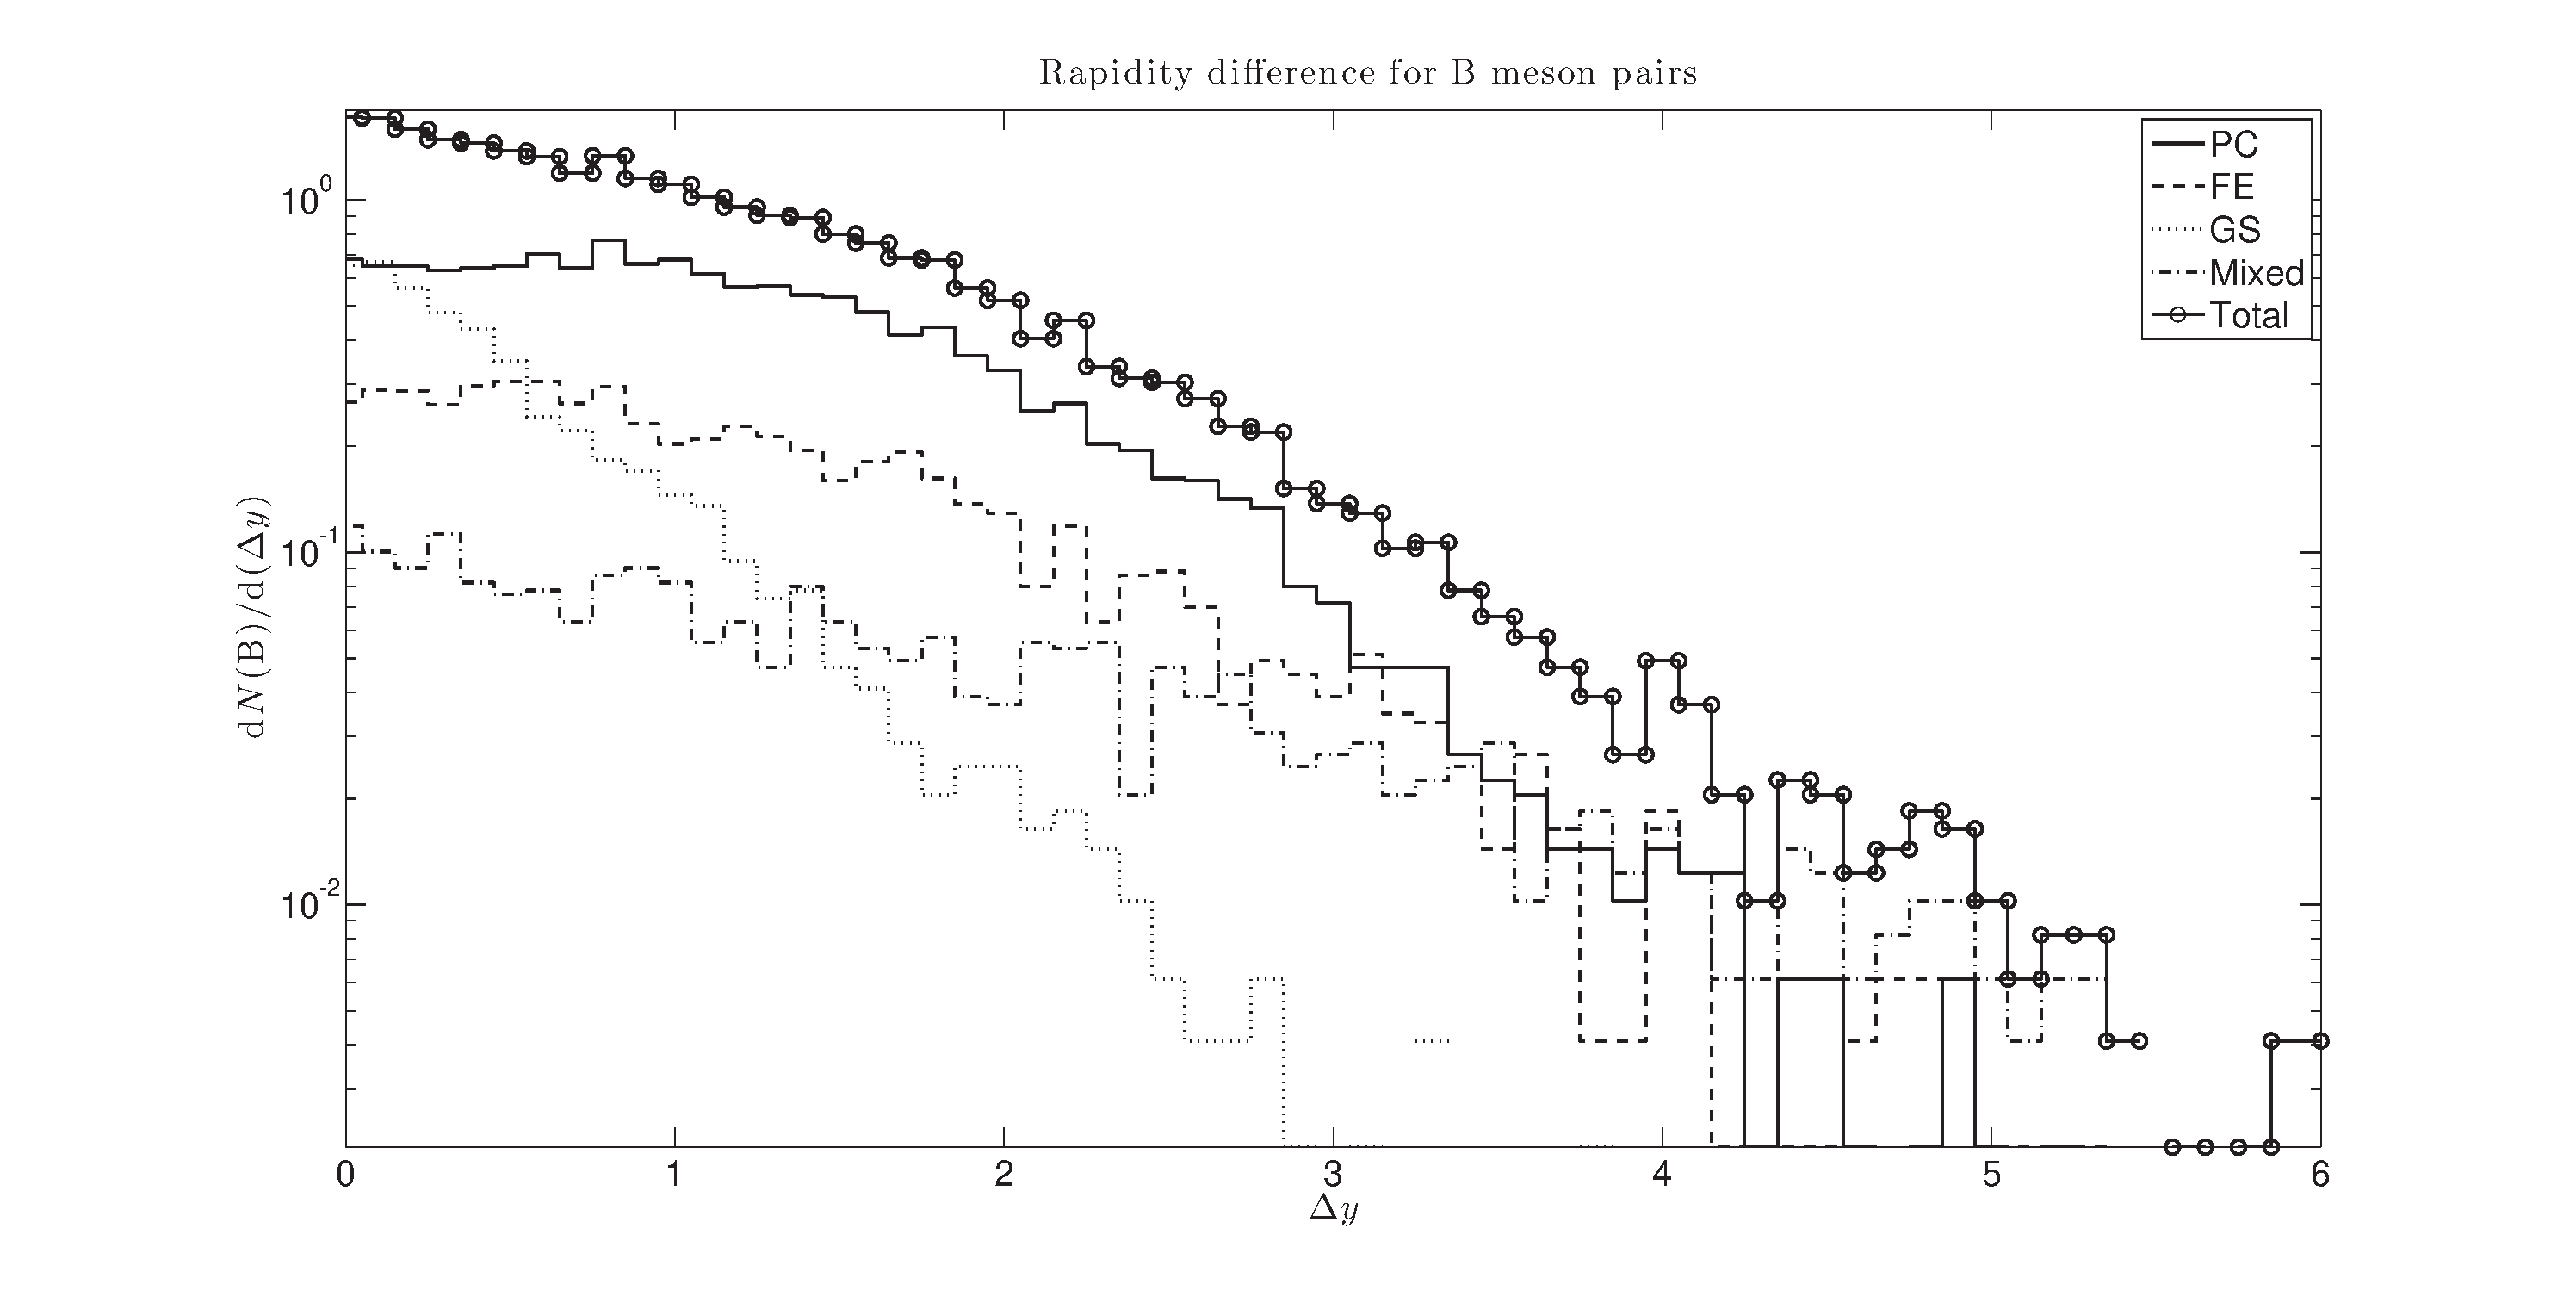
\includegraphics[width=15cm]{BBYOp1}
\label{fig:BBYOp1}
\end{figure}

\begin{figure}[!h]
\centering
\caption[[Rapidez relativa de pares de mesones $\B$. Cuatro opciones de \textsc{Pythia}.]{Rapidez relativa de pares de mesones $\B$ usando la opciones de \textsc{Pythia}:  1 (sólida), 2 (líneas), 3 (puntos) y 4 (líneas y puntos).}
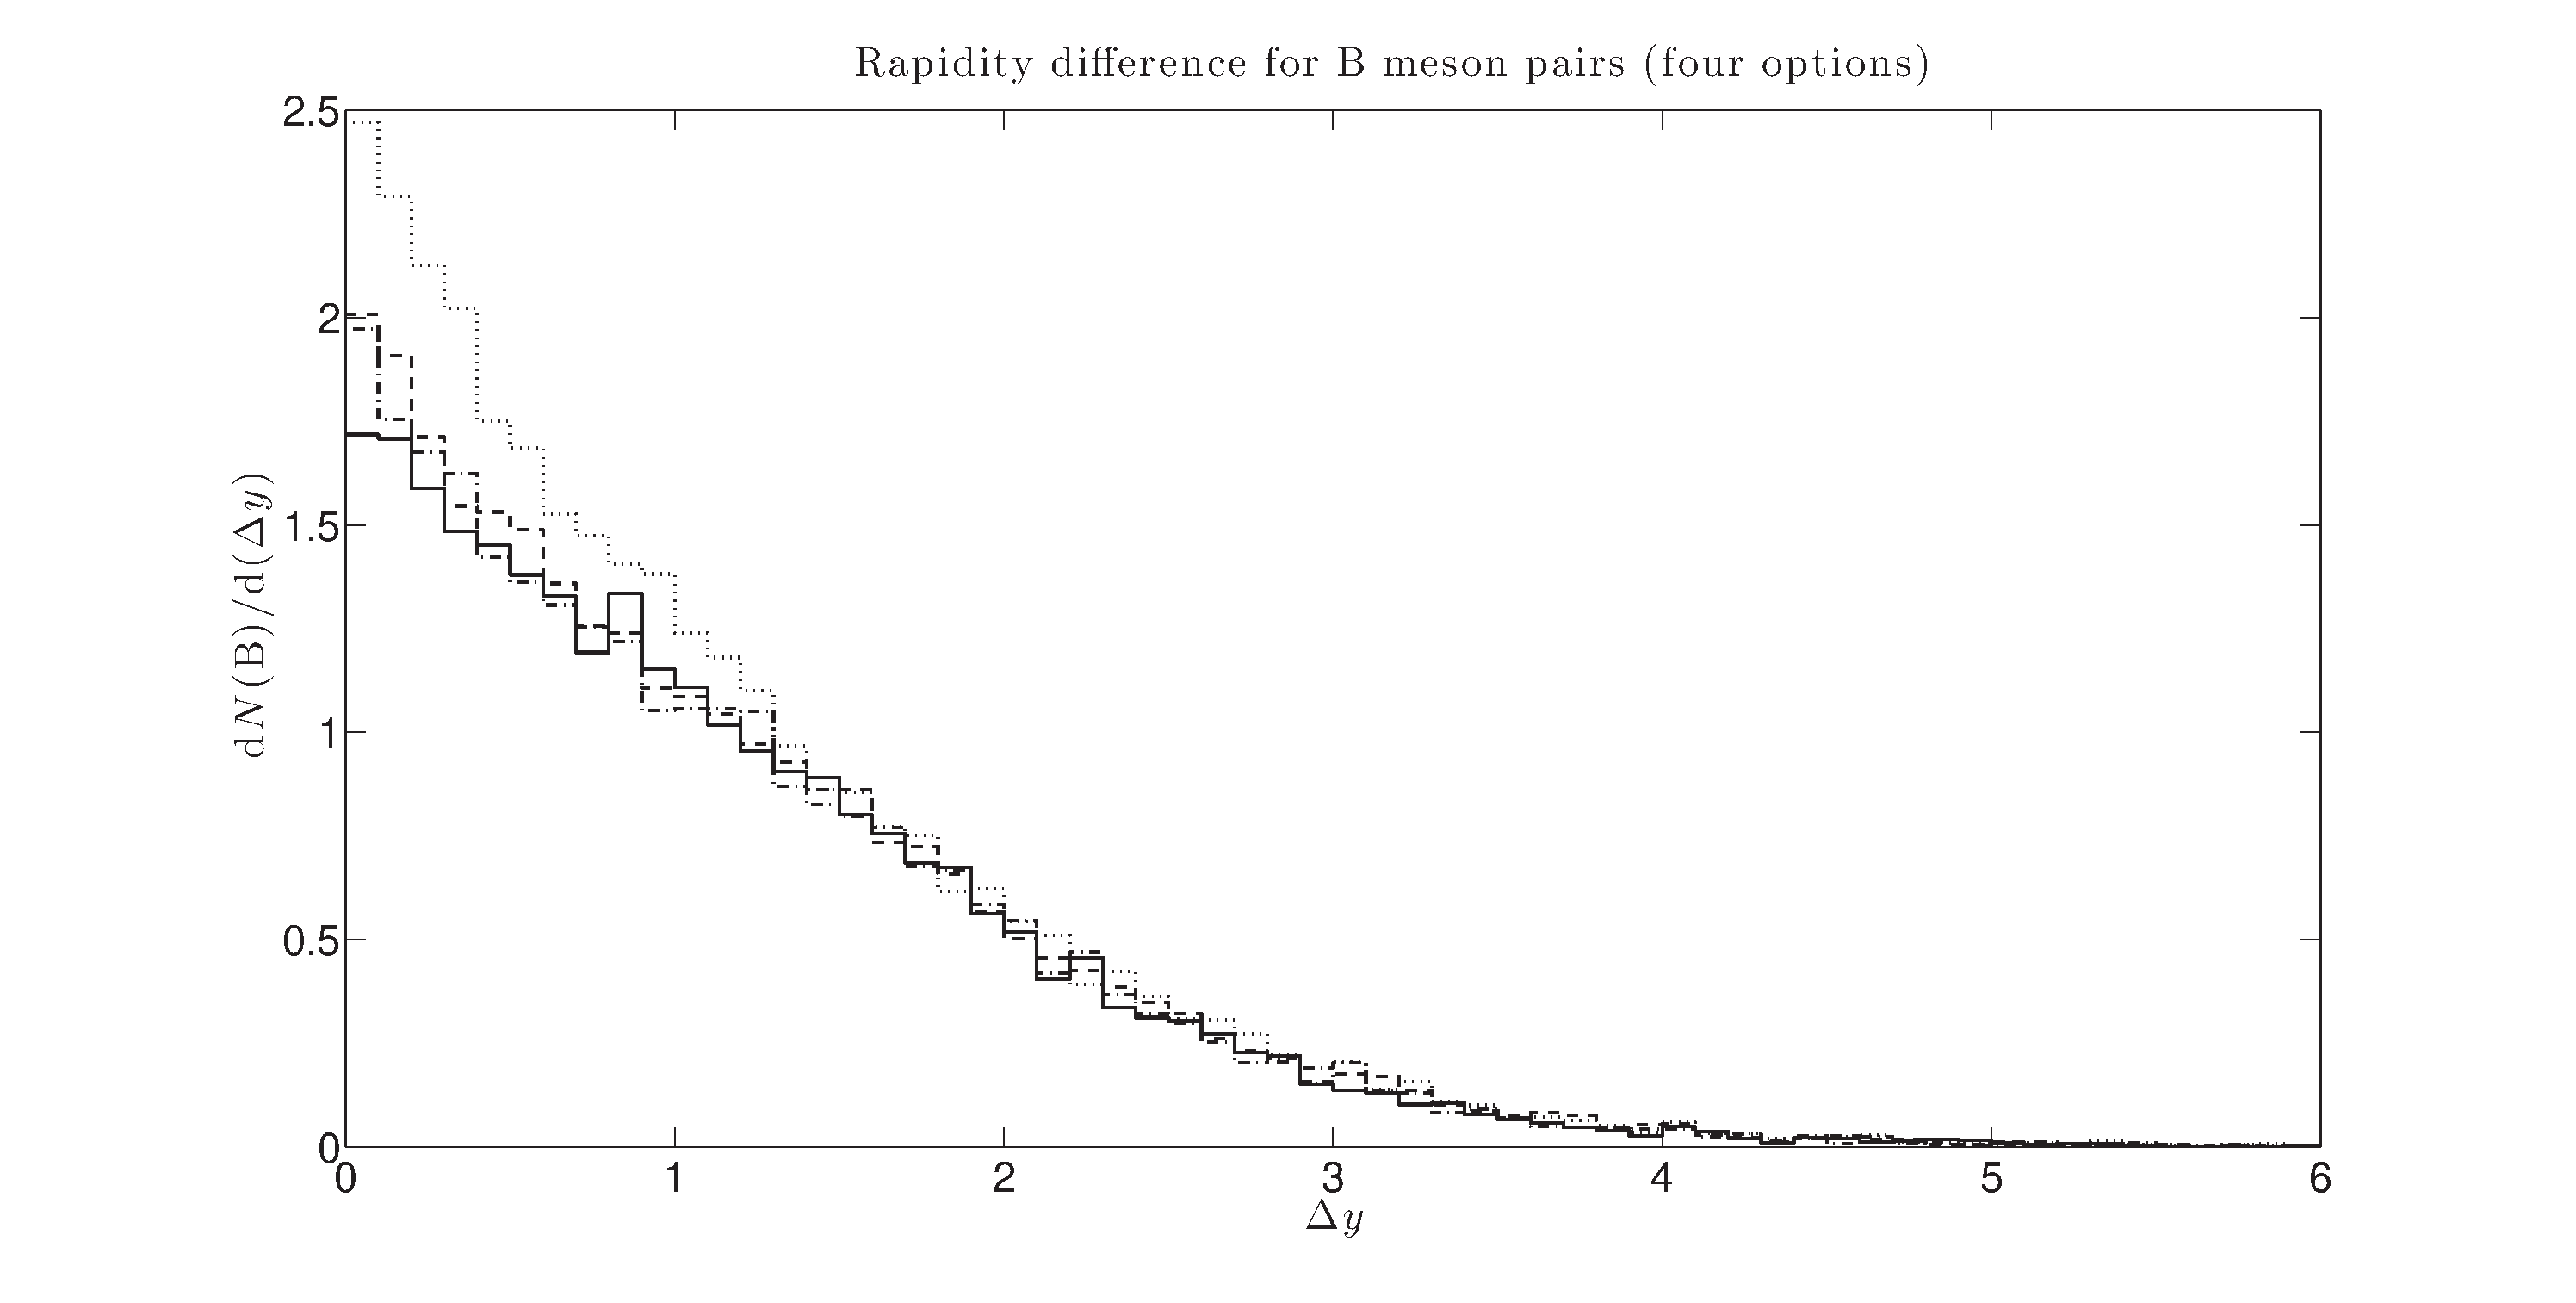
\includegraphics[width=15cm]{BBY4Op}
\label{fig:BBY4Op}
\end{figure}

Diferencias bajas en rapidez significan que las partículas en los pares están cercanas en ``distancia polar'', al mismo tiempo que un $\Delta y$ alto significa una separación polar alta. En principio, los quarks provenientes de PC son producidos con una diferencia de rapidez muy pequeña, pero los efectos cinemáticos de la lluvia de partones abren esta separación y los correspondientes mesones contribuyen significativamente en valores medianos y bajos de $\Delta y$.

La contribución de FE es menos importante que la proveniente de PC. La producción por excitación de sabor cae por debajo de GS únicamente a diferencias de rapidez bajas.

El cambio en las opciones es entonces apreciable a valores bajos de $\Delta y$, mientras que en la región media y en la cola final el comportamiento es similar en las cuatro opciones.

\subsection{Distancias $R$}

La cantidad $R$ contiene información de las dos variables estudiadas anteriormente. En cierto sentido, al dar valores de $\Delta y$ y $\Delta \varphi$ de un par de mesones, se tiene una descripción completa (Lorentz invariante ante boosts en $z$) de la distribución angular del par. En el plano $y - \varphi$ la distancia (también invarinte) $R=\sqrt{(\Delta y)^2 + (\Delta \varphi)^2}$ es útil para agrupar los pares con sus ``vecinos'' angulares. Para definir un \textit{jet de partículas} se usa típicamente la distancia $R$ para agrupar hadrones cercanos.

La figura \ref{fig:BBROp1} muestra el comportamiento de cada fuente, más la producción total de mesones $\B$ para la opción 1.
\begin{figure}[!h]
\centering
\caption[Distancia $R$ de pares de mesones $\B$. Opción por feceto de \textsc{Pythia}.]{ Distancias $R$ de pares de mesones $\B$ usando la opción por defecto de \textsc{Pythia}, incluyendo las cuatro fuentes de producción.}
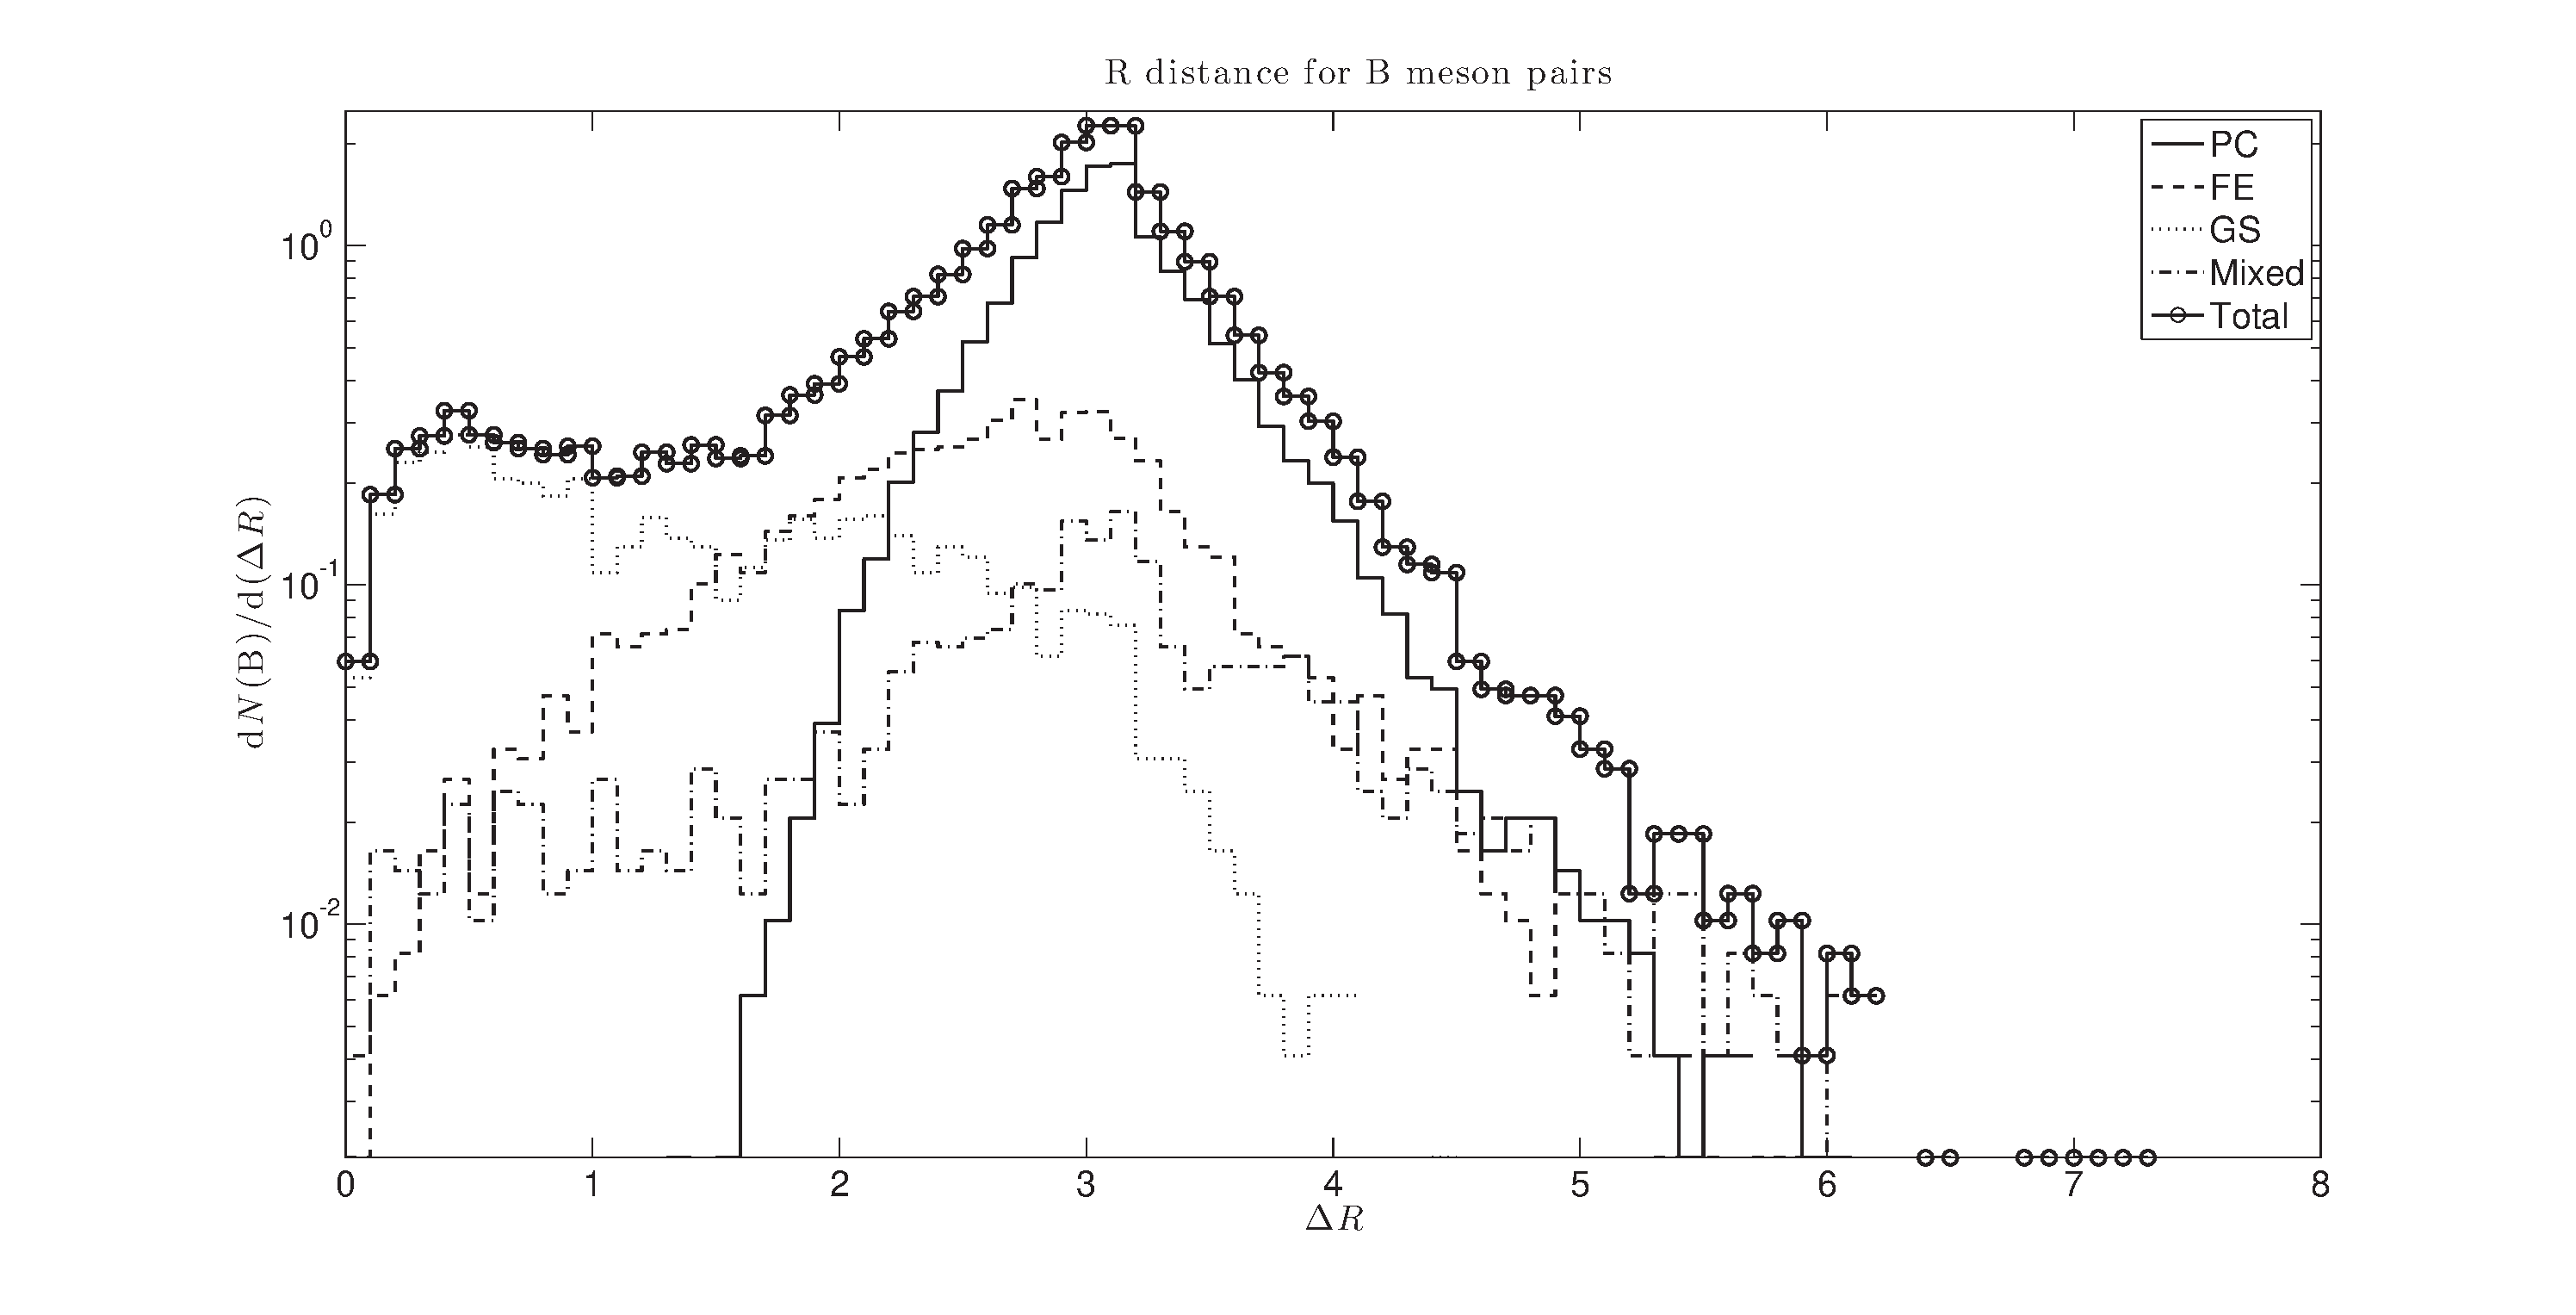
\includegraphics[width=15cm]{BBROp1}
\label{fig:BBROp1}
\end{figure}
Debido a la contribución relevante de PC a ángulos azimutales de abertura grandes, el pico principal de la distancia $R$ es cercano al valor de $\pi$. La excitación de sabor también presenta un crecimiento cerca de ese valor, aunque es menos significativo. Los mesones producidos en GS están usualmente cercanos tanto en $y$ como en $\varphi$, así que los pares clasificados como ramificación de un gluón serán probablemente agrupados en el mismo jet.
\begin{figure}[!h]
\centering
\caption[Distancia $R$ de pares de mesones $\B$. Cuatro opciones de \textsc{Pythia}.]{Distancias $R$ de pares de mesones $\B$ usando las opciones  de \textsc{Pythia}:  1 (sólida), 2 (líneas), 3 (puntos) y 4 (líneas y puntos).}
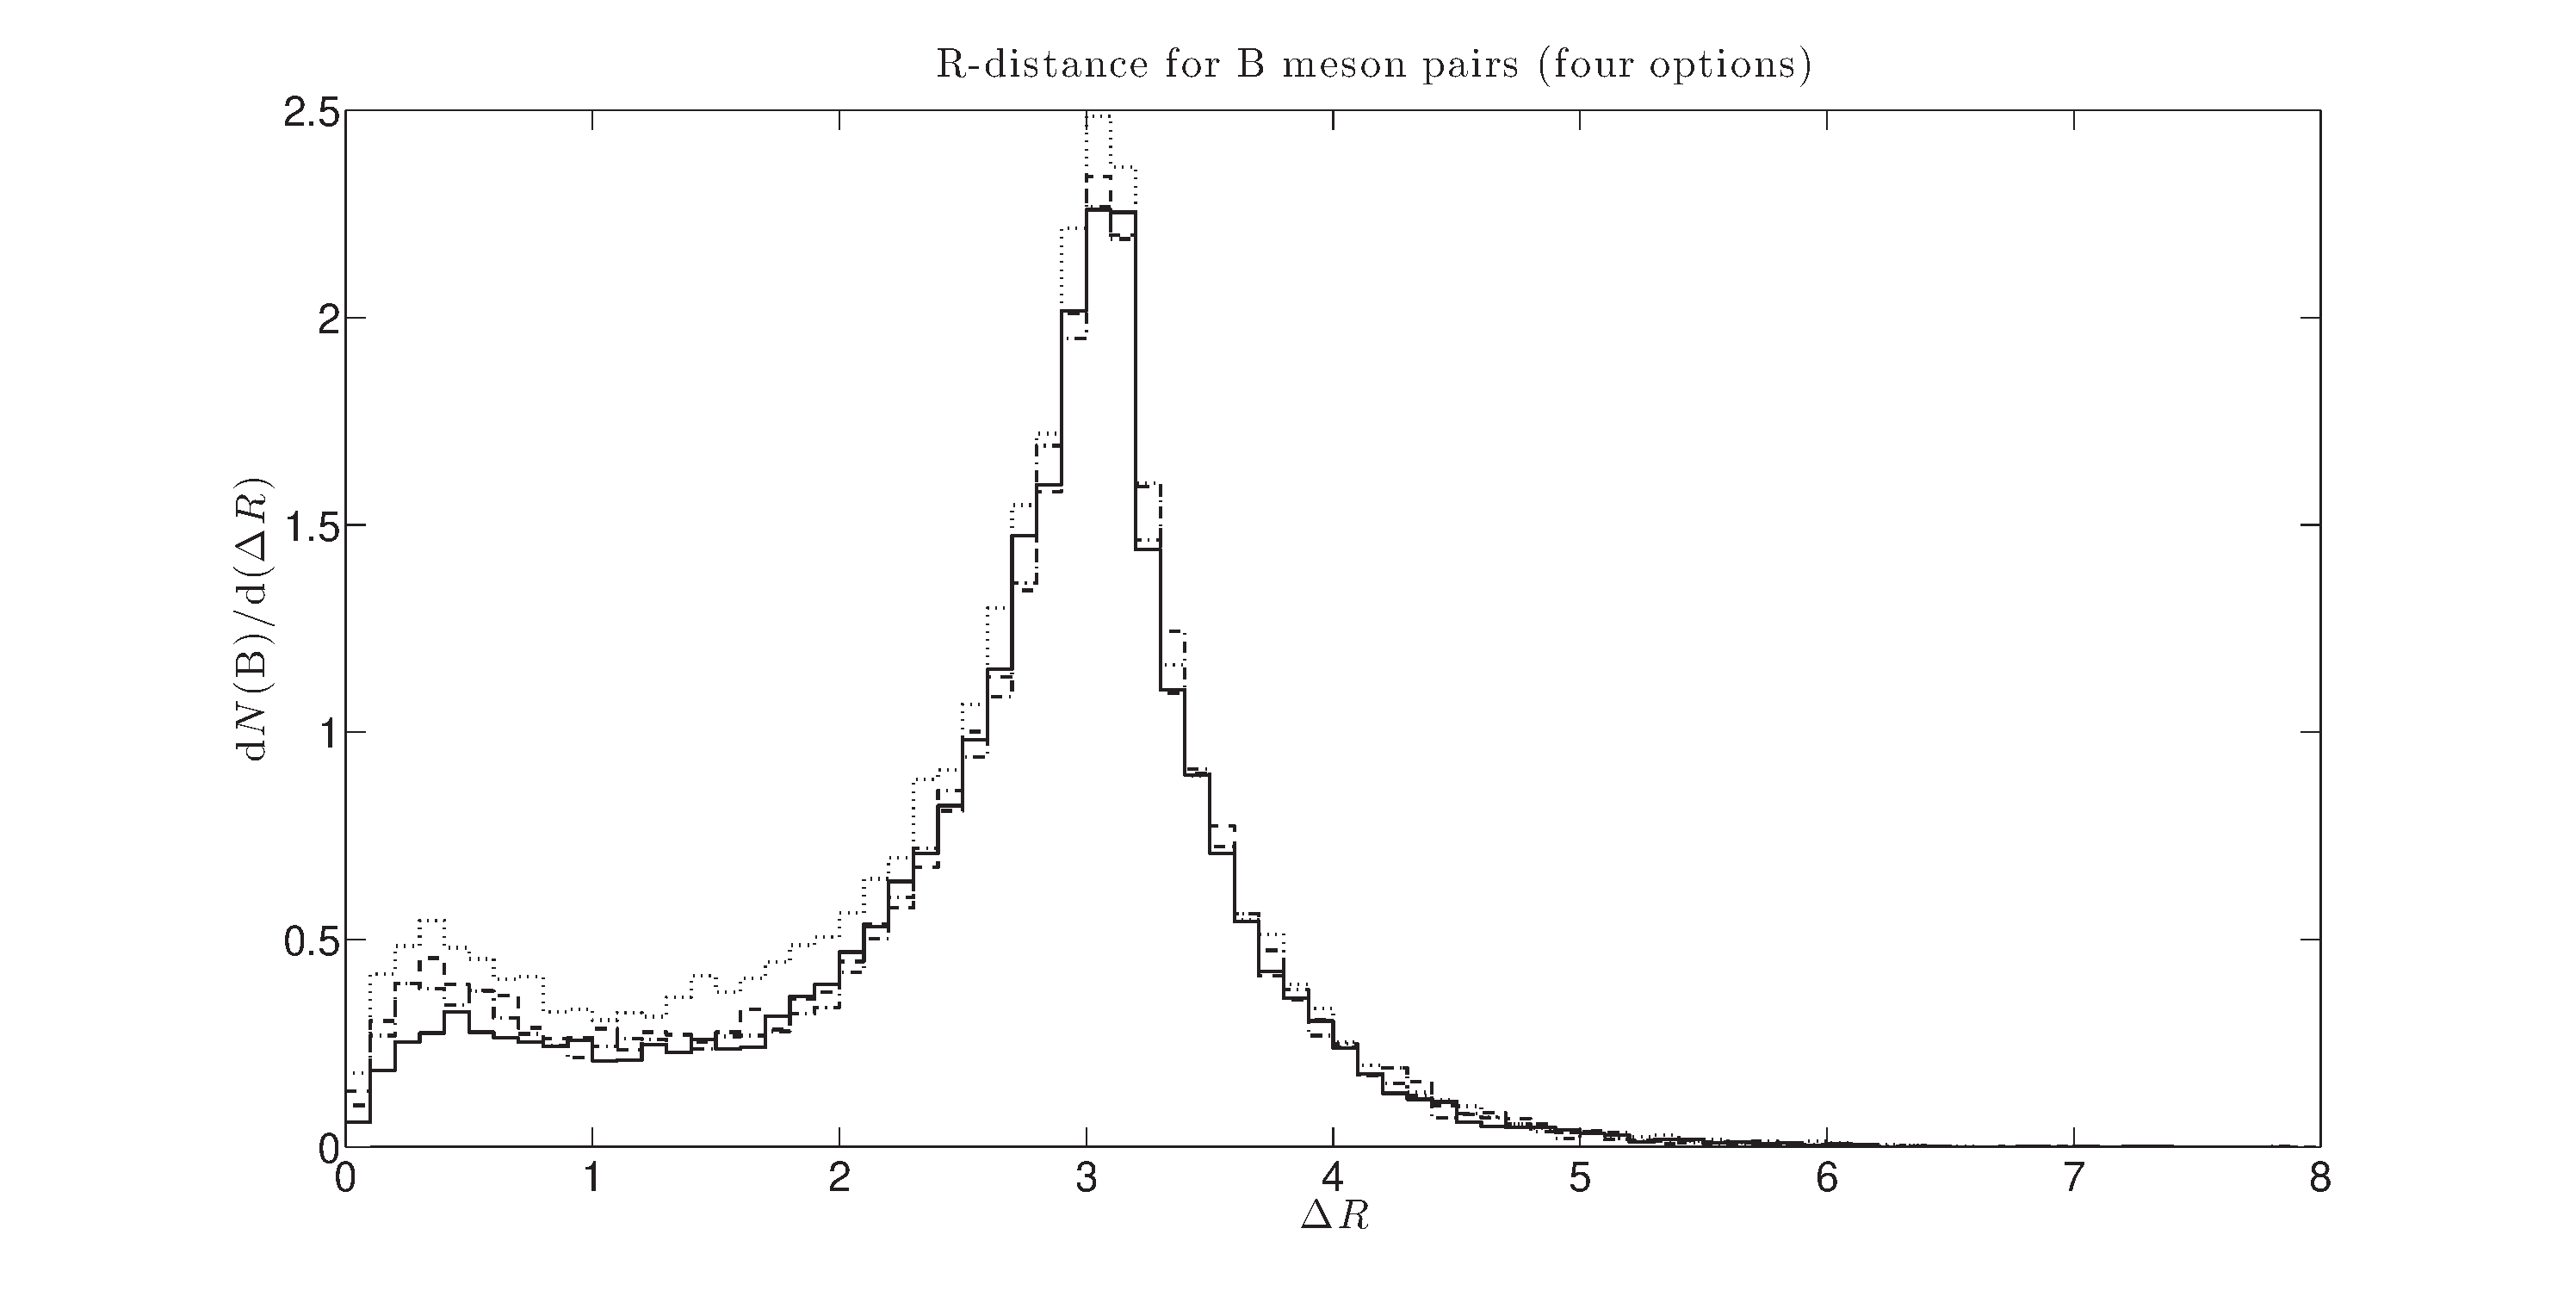
\includegraphics[width=15cm]{BBR4Op}
\label{fig:BBR4Op}
\end{figure}

Debido a que $R$ combina la información de la rapidez relativa y la abertura angular, se espera un aumento respectivo en cada una de las opciones a distancias pequeñas, que se muestra en la figura \ref{fig:BBR4Op}.

Datos experimentales sobre las correlaciones angulares de bottom pueden ser conseguidas en \cite{Khachatryan:2011wq} y \cite{ATLAS:2011ac}. Los análisis hechos ahí están incluidos en un conjunto de rutinas de validación de Rivet \cite{Buckley:2010ar}. La integración entre análisis de \textsc{Pythia} y Rivet, y la producción de datos a partir de esta, fue una maquinaria considerada para este trabajo, aunque no se logró implementar completamente debido a restricciones en el tiempo. El estudio de colisiones hadrónicas puede ser llevado a cabo también para diferentes PDFs, para observar el impacto en los mecanismos de producción y luego comparar con datos experimentales.

Existen también estudios sobre la producción de quarks $\b$ en el Tevatron (colisiones $\p\pbar$ a 2000 GeV), un ejemplo de estos es \cite{vallecorsa}.

\chapter{Conclusiones}
\label{sec:summary}

La tasa de producción $\g_{\b\bbar}$ fue simulada y comparada con resultados experimentales. Los resultados están de acuerdo con la opción por defecto de \textsc{Pythia} y con la opción 4 dentro de los errores experimentales. Curiosamente, el aumento producido por la opción 4 en la región de umbral de masa es casi exactamente cancelado por la supresión a masas altas, lo que conllevó a una tasa cercana a la dada por la opción por defecto. La opción 2 da un resultado dentro de dos desviaciones estándar comparado con los datos experimentales, mientras que la opción 3 no parece reproducir la tasa. Las opciones 5-8, usando $m^2$ como el argumento  del acoplo fuerte, no afecta sensiblemente la tasa (alrededor de 5\% de diferencia para cada opción).

Existe un limitado conjunto de datos disponibles para el estudio de quarks pesados en colisionadores leptónicos. Futuras mediciones de la producción de quarks pesados como función de la masa invariante del par pudiera esclarecer cuál de las opciones es la más adecuada, o la necesidad de una nueva.

El estudio no permite concluir definitivamente sobre la base del espectro de energía de los mesones $\D^{*\pm}$. La opción por defecto muestra una deficiencia a bajas energías que pudiera ser corregida por el aumento dado por las opciones alternativas, particularmente por la opción 3. Sin embargo, todas las opciones presentan un exceso a energías medianas que, de ser corrido a regiones de más bajas energías a través de, por ejemplo, un nuevo modelado del decaimiento $\B\to\D$, pudiera también reconciliar \textsc{Pythia} y los datos experimentales, sin introducir una nueva tasa de producción $\g\to\Q\Qbar$.

Para colisiones protón-protón a energías típicas del LHC, la abertura angular azimutal, las rapideces relativas y las distancias $R$ de pares de mesones $\B$ fueron simuladas. Las contribuciones de los mecanismos de producción a las cantidades mencionadas fueron mostradas. La variación de los observables usando las diferentes opciones de \textsc{Pythia} también fue estudiada y mostrada en los gráficos. Usando cortes inferiores para el momentum transveso para la generación de eventos y para los mesones $\B$ analizados, los eventos seleccionados fueron alrededor de $1.5$ \% de los generados.

Futuros estudios pudieran empezar comparando los resultados simulados de las cuatro opciones con los datos. Existen resultados experimentales y análisis para los experimentos Tevatron y LHC, basados en diferentes mecanismos de reconstrucción de eventos. La dependencia de las correlaciones y tasas de producción  implementando otras PDFs pueden ser también exploradas en este contexto.




%\tableofcontents
%
%\newpage
%
%\chapter*{Introducción}
\label{sec:introduction}

Una de las mayores búsquedas de la física del último centenar de años ha consistido en obtener un entendimiento de cómo el mundo funciona a la escala más pequeña, lo que ha llevado a notables descubrimientos. Con la ayuda de modelos matemáticos somos capaces de describir y predecir muy precisamente algunos fenómenos físicos observados, tales como el átomo y sus transiciones de energía, reacciones y decaimientos nucleares, por sólo nombrar un par de ellos.

La simple idea de hacer colisionar pequeñas partículas ha jugado un rol importante en esos descubrimientos y ha contribuido en gran medida al entendimiento de las leyes físicas a esa escala. Además, con la aparición de máquinas cada vez más poderosas, hemos sido capaces de observar con mejor detalle los componentes fundamentales de la naturaleza. Esto es análogo a la luz: su energía es inversamente proporcional a su longitud de onda, de manera que se requiere de mayor energía para resolver objetos más pequeños.

Los colisionadores de partículas se han convertido en los caballos de batalla de los físicos de partículas. Usando campos eléctricos y magnéticos, estas máquinas aceleran y curvan haces de partículas que luego colisionarán en lugares específicos, en donde están dispuestos detectores para observar el resultado de la interacción. Debido a que las partículas que chocan son muy pequeñas y las energías muy altas, el tratamiento matemático debe ser tanto mecánico-cuántico como relativista.

Dentro del actual marco de trabajo matemático-analítico (formalmente llamado el Modelo Estándar (ME)), sólo es posible manejar interacciones simples que involucran pocas partículas. Un tratamiento diferente es necesario para hacer los cálculos inherenetes a los procesos reales que ocurren en los colisionadores, donde típicamente cientos de partículas son creadas. Los programas de computadoras llamados ``generadores de eventos'' han venido siendo desarrollados para tratar tales situaciones de una manera fenomenológica, haciendo uso de modelos ajustables, inspirados tanto en predicciones teóricas como en resultados experimentales para ajustarse mejor a los datos. Además, los generadores han sido utilizados para explorar escenarios posibles, antes de que los experimentos reales sean montados y sus respectivos análisis llevados a cabo.

El estudio de una de las fuerzas fundamentales de la naturaleza, la interacción fuerte, es de particular interés en este trabajo. El campo ``gluónico'' proveniente de la interacción fuerte mantiene unidos a los quarks dentro de compuestos llamados hadrones, como los protones o neutrones. En las colisiones de altas energías, la interacción fuerte es la dominante, y a partir de ella (y de su campo gluónico) es posible crear pares de quarks de tipos más pesados que los que se encuentran en los protones y neutrones. El estudio de los hadrones que contienen estos quarks pesados puede ampliar nuestro conocimiento sobre cómo actúa dicha fuerza.

El generador de eventos \textsc{Pythia} (\cite{Sjostrand:2006za}, \cite{Sjostrand:2007gs}) será usado para analizar los diferentes mecanismos de producción de quarks y su rol en las colisiones. Varias modificaciones al algoritmo que usa PYTHIA para modelar la tasa de producción de pares $\g\to\Q\Qbar$ con $\Q$ un quark pesado (de tipo charm ($\c$) o bottom ($\b$)) han sido propuestas y serán probadas. La teoría subyacente es descrita en el capítulo \ref{sec:theoretical}.

El estudio de los mecanismos de producción comprende dos partes: colisiones electrón-positrón a energía de resonancia del $Z^0$ para comparar con datos del Gran Colisionador de Electrones y Positrones (LEP, por su sigla en inglés) y las más complicadas colisiones de hadrones, a energías típicas del Gran Colisionador de Hadrones (LHC). Varios observables físicos serán estudiados, como la separación angular de los objetos producidos a partir de los quarks pesados de las colisiones.

Gracias a que el generador provee una historia detallada del proceso simulado, se pueden trazar los orígenes de cada partícula y clasificarla. Los métodos para analizar los eventos son discutidos en el capítulo \ref{sec:analysis}. En algunos casos, los resultados (sección \ref{sec:results}) serán comparados con datos experimentales. Un resumen final y las perspectivas para futuros estudios se encuentran en el capítulo \ref{sec:summary}.



%
%\chapter{Resumen teórico}
\label{sec:theoretical}

El ME es la teoría física  que explica las propiedades de la materia y sus interacciones en su nivel más fundamental. Utilizando el marco de trabajo de la teoría especial de la relatividad y la mecánica cuántica, el ME lidia con las partículas elementales de la realidad física.

Las partículas pueden ser clasificadas de diferentes maneras, de acuerdo a sus propiedades, como el espín, la carga eléctria y la masa. Se puede hacer una primera distinción a partir de los valores de espín. Partículas con espín entero\footnote{Aquí y en el resto del trabajo, usaremos las unidades naturales: $\hbar$ (constante de Planck reducida) = $c$ (velocidad de la luz) = $e$ (carga del electrón) = 1.} son llamadas \textbf{bosones} y son las que median las interacciones, mientras que las que tienen espín semientero son llamadas \textbf{fermiones} y representan las partículas que interactúan. Por otra parte, para cada partícula del ME existe una antipartícula con las mismas propiedades pero cargas opuestas. Los fermiones son creados (y aniquilados) necesariamente en pares materia-antimateria, mientras que las interacciones son mediadas por los bosones, creados usualmente de manera individual.

Cuatro fuerzas fundamentales son actualmente conocidas en la naturaleza: las fuerzas nucleares fuerte y débil, el electromagnetismo y la gravedad. (Las primeras tres de ellas son descritas por el ME, mientras que la última aún no ha sido consistentemente incluida en dicho modelo.) La tabla \ref{table:SMBoson} lista las interacciones con sus respectivos bosones mediadores, es decir, las partículas asociadas al campo de la interacción.

\begin{table}[!h]
\caption{Interacciones en el Modelo Estándar y sus respectivos bosones.}\smallskip
\label{table:SMBoson}
\centering 

\begin{tabular}{cc}
\hline \hline  
\smallskip
Fuerza& Bosón (masa en GeV\cite{Beringer:1900zz}) \\ 
\hline
Electromagnetismo & $\gamma$ (0) \\
Interacción débil & $W^\pm$ y $Z^0$ ($80.4$ y $91.2$) \\
Interacción fuerte & $\g$ (0) \\
\end{tabular}
\end{table}


Además de la carga eléctrica, existen una carga para la fuerza fuerte llamada ``carga de color'', en analogía con el color de la vida cotidiana, como veremos luego. Los fotones ($\gamma$) y bosones $Z^0$ no tienen carga, de modo que son sus propias antipartículas, mientras que los gluones poseen sólo carga de color y los bosones $W^\pm$ tienen ($\pm 1$) carga eléctrica. Entonces, las antipartículas de los gluones son gluones con contenido de color opuesto, mientras que los bosones $W^+$ y $W^-$ son sus respectivas antipartículas.

Un bosón adicional no está incluido en la lista de la tabla 1, que es el bosón de Higgs (125 GeV), este bosón media el mecanismo de obtención de masa de las partículas. El universo está lleno del campo escalar neutro de Higgs, que tiene un valor de expectación no nulo en el vacío por el rompimiento espontáneo de la simetría del campo. Luego, las partículas interactúan con este campo y obtienen su masa. 

Hasta los momentos, 12 fermiones (y sus respectivas antipartículas) han sido observados, tal y como se muestran en la tabla 2. Cada columna en la tabla es llamada una \textbf{generación} o \textbf{familia}. Las segunda ($\c,\s,\mu,\nu_\mu$) y tercera ($\t,\b,\tau,\nu_\tau$) familias son ``versiones pesadas'' de la primera ($\u,\d,e,\nu_e$). Los neutrinos (en la última fila) son prácticamente no-masivos, los resultados experimentales han dado sólo un límite superior para sus masas. La carga eléctrica de cada quark en la primera fila es 2/3, mientras que los de la segunda fila tienen -1/3; los leptones de la tercera fila tienen carga -1 y sus neutrinos ($\nu$) son eléctricamente neutros.

A pesar de que todas las parículas hasta ahora mecionadas existen, los átomos están hechos únicamente de fermiones de la primera generación. El electromagnetismo mantiene a los electrones alrededor del núcleo, compuesto de neutrones y protones. Los últimos dos son combinaciones de quarks: ``udd'' y ``udd'' respectivamente. Protones, neutrones y otros objetos compuestos de tres (anti)quarks son conocidos como (anti)bariones, mientras que las combinaciones quark-antiquark dan lugar a mesones. Los bariones y mesones tienen el nombre genérico de hadrones.

Las partículas de la segunda y tercera familia son inestables y existen por lapsos cortos, decayendo luego a materia de la primera generación. Por ser más pesada, mayor energía es requerida para producir materia de este tipo; por eso es posible detectarla sólo en experimentos de altas energías, como colisionadores, y estudiando procesos cósmicos lo suficientemente energéticos.

Los quarks también interactúan a través de la fuerza fuerte, ya que tienen carga de color, a diferencia de los leptones (sin color). Por analogía con el color usual, existen tres tipos de carga básica involucradas en la interacción fuerte, llamados rojo ($r$), verde ($g$) y azul ($b$); y juntos pueden formar una combinación sin color (un singlete de color, en términos precisos) de la misma manera en que estos colores cotidianos sumados resultan en blanco. Esto significa que existen superposiciones mecánico-cuánticas que resultan en estados de singletes de color. Además, los anticolores son tales que se anulan cuando se combinan con su correspondiente color (por ejemplo, la combinación de rojo con anti-rojo ($r+\bar{r}$) debe ser neutral en color). Como dijimos anteriormente, los gluones también transportan carga de color, que transfieren durante las interacciones.

El contenido de color de los gluones es algo más complicado que el de los quarks, y esto se debe a la estructura de grupo de la teoría. Los gluones contienen un combinación no nula de color-anticolor. Teniendo 3 colores independientes, es natural tener los índices de color corriendo de 1 a 3 y una representación de matrices $3\times3$, como veremos en la siguiente sección. El grupo de simetría asociado con la fuerza fuerte es $SU(3)$, que tiene $3^2-1=8$ generadores linealmente independientes. Al sustraer uno, lo que estamos haciendo es excluir el generador que corresponde al estado de singlete. Así, los gluones son llamados ``octetos de color''.

Debido a que el color debe ser conservado, los gluones cargan una configuración no nula tal que puedan transmitir color y resultaren una nueva configuración ``coloreada'' de quarks o gluones luego de la interacción. Por ejemplo, el contenido de color de una emisión de un gluón por un quark rojo pudiera ser: $\q(r)\to\q(b)+\g(r\bar b)$.

Todos los hadrones en la naturaleza han sido observados como singletes de color. Así, existen varias maneras de producir tales estados, siendo las más comunes: la combinación de tres (anti)colores en un singlete para formar un (anti)barión, y la combinación de un quark con un antiquark en una combinación color-anticolor para formar mesones. La fuerza fuerte actúa sólo en objetos con carga de color; esto significa que la fuerza fuerte no es exclusivamente de los quarks, sino que también los gluones pueden interactuar con otros gluones. Este último proceso puede ser visto como sigue: nombrando a los gluones iniciales 1 y 4, luego 1 se divide en dos nuevos gluones, a los que llamaremos 2 y 3 ($\g(1)\to\g(2)+\g(3)$), el último de los cuales finalmente se une con 4 para formar un nuevo gluón, 5 ($\g(3)+\g(4)\to\g(5)$). Este proceso puede ser ilustrado por la figura \ref{fig:gluonGluon}, que es un ejemplo de los llamados diagramas de Feynman.

\begin{fmffile}{GluonGluon}

\begin{figure}[h]
  \centering
%(along, up)
    \begin{fmfgraph*}(150,100)
      \fmfstraight
      \fmfleft{i1,i2}
      \fmfright{o1,o2}
      \fmf{phantom}{i1,w1,w2,o1}
      \fmf{gluon,label=$\g(1)$}{i1,w1}
      \fmf{gluon,label=$\g(2)$}{w1,o1}
      \fmf{phantom}{i2,w3,w4,o2}
      \fmf{gluon,label=$\g(4)$}{i2,w4}
      \fmf{gluon,label=$\g(5)$}{w4,o2}
      \fmf{gluon,label=$\g(3)$}{w1,w4}
    \end{fmfgraph*}
\caption[Gluon-gluon interaction]{Diagrama de Feynman para una interacción gluón-gluón.}
\label{fig:gluonGluon}
\end{figure}

\end{fmffile}

Estos diagramas representan las interacciones del ME. Las partículas son dibujadas como líneas y las interacciones son los vértices. Los fermiones son representados usualmente por líneas rectas sólidas, mientras que los bosones por líneas rizadas (gluones), onduladas ($W, Z, \gamma$) o punteadas (Higgs). Tal y como sugiere el párrafo anterior, el tiempo fluye de izquierda a derecha en el diagrama. A pesar de que los diagramas de Feynman no representan las trayectorias reales de las partículas, estos constituyen una herramienta poderosa para describir la naturaleza de las interacciones y hacer cálculos de elementos de matriz, que serán descritos más tarde.

Dos características relevantes de la fuerza fuerte son:

\paragraph{Confinamiento} Debido a que los quarks individualmente no pueden formar un singlete de color, no se ha observado hasta ahora ningún quark libre. A distancias mayores a $10^{-15}$ m, se cree que la fuerza fuerte por intercambio de gluones es constante, así que la energía almacenada entre quarks crece linealmente con la distancia cuando se intenta separarlos para descomponer un hadrón. Para ilustraar esto, tomaremos el ejemplo simple de un mesón: cuando se da al sistema suficiente energía para separar a los dos quarks, el campo gluónico creará un nuevo par quark-antiquark entre ellos. De esta manera, la interacción original será apantallada, formando dos nuevos mesones, es decir, cada quark de los extremos interactuará sólo con su vecino más cercano del nuevo par. Entonces este proceso asegura que todos los quarks permanecerán confinados en hadrones.

\paragraph{Libertad asintótica} La fuerza fuerte cambia su comportamiento a distancias muy pequeñas. En ese caso, ésta es menos fuerte y los quarks interactúan de una manera más débil. Los quarks tienden entonces asintóticamente a ser objetos libres. De ese modo, la teoría puede ser tratada perturbativamente, como veremos en la sección \ref{subsec:QCDLag}.

\section{El Lagrangiano del Modelo Estándar y los elementos de matriz}
\label{subsec:QCDLag}

La parte del modelo estándar que trata la interacción fuerte es llamada Cromodinámica Cuántica (QCD, por su sigla en inglés). La intensidad y las reglas de las interacciones están explícitamente expuestas en el lagrangiano. Los procesos en los que estamos interesados son los que involucran interacciones entre quarks y gluones. La parte del lagrangiano para estas interacciones tiene la forma \cite{Kane:1993}:

 \begin{equation}
  \frac{g_s}2 \qbar_\alpha \gamma^\mu \lambda^a_{\alpha \beta} G_\mu^a \q_\beta\label{eq:QCDLag}
  \, .
\end{equation}

En la fórmula, $g_s$ es la intensidad del acoplamiento de la fuerza fuerte. Tanto $\q_\beta$ como $\qbar_\alpha$ son estados espinoriales de los quarks con sus respectivos índices de color ($\alpha,\beta = 1,2,3$), $\gamma^\mu$ representa una matriz de Dirac y $\lambda^a_{\alpha\beta}$ la matriz de color de Gell-Mann, que son los generadores del grupo SU(3). $G_\mu^a$ es la intensidad del campo gluónico. El índice $\mu$ es espacio-temporal (0,1,2,3), mientras que el índice del campo gluónico $a=1,...,8$. El lagrangiano completo del ME también comprende los términos de masa y las autointeracciones de los gluones.

Físicamente, la expresión (\ref{eq:QCDLag}) representa los siguiente mecanismos: emisión de un gluón por un quark ($\q\to\g\q$), absorción de un gluón por un quark ($\g\q\to\q$) y creación de un par a partir de un gluón ($\g\to\qbar\q$); además de los correpondientes procesos invertidos en el tiempo: absorción de un gluón por un antiquark ($\g\qbar\to\qbar$), emisión de un gluón por un antiquark ($\qbar\to\g\qbar$) y aniquilación de un par en un gluón ($\q\qbar\to\g$).

\begin{fmffile}{feyndiag}

\begin{figure}[h]
  \centering
%(along, up)
    \begin{fmfgraph*}(100,100)
      \fmfleft{i1}
      \fmfright{o1,o2}
      \fmf{fermion,label=$\q$}{i1,w1}
      \fmf{fermion,label=$\q$}{w1,o1}
      \fmf{gluon,label=$\g$}{o2,w1}
    \end{fmfgraph*}
    \hspace{2em}
    \begin{fmfgraph*}(100,100)
      \fmfleft{i1,i2}
      \fmfright{o1}
      \fmf{fermion,label=$\q$}{i1,w1}
      \fmf{gluon,label=$\g$}{i2,w1}
      \fmf{fermion,label=$\q$}{w1,o1}
    \end{fmfgraph*}
    \hspace{2em}
    \begin{fmfgraph*}(100,100)
      \fmfleft{i1}
      \fmfright{o1,o2}
      \fmf{gluon,label=$\g$}{w1,i1}
      \fmf{fermion,label=$\q$}{w1,o1}
      \fmf{fermion,label=$\qbar$}{o2,w1}
    \end{fmfgraph*} \\
    \vspace{3em}
        \begin{fmfgraph*}(100,100)
      \fmfleft{i1,i2}
      \fmfright{o1}
      \fmf{fermion,label=$\qbar$}{w1,i1}
      \fmf{gluon,label=$\g$}{i2,w1}
      \fmf{fermion,label=$\qbar$}{o1,w1}
    \end{fmfgraph*}
    \hspace{2em}
    \begin{fmfgraph*}(100,100)
      \fmfleft{i1}
      \fmfright{o1,o2}
      \fmf{fermion,label=$\qbar$}{w1,i1}
      \fmf{fermion,label=$\qbar$}{o1,w1}
      \fmf{gluon,label=$\g$}{o2,w1}
    \end{fmfgraph*}
    \hspace{2em}
    \begin{fmfgraph*}(100,100)
      \fmfleft{i1,i2}
      \fmfright{o1}
      \fmf{fermion,label=$\qbar$}{w1,i1}
      \fmf{fermion,label=$\q$}{i2,w1}
      \fmf{gluon,label=$\g$}{o1,w1}
    \end{fmfgraph*}
\caption[QCD quark diagrams]{Diagramas de Feynman para los procesos representados por la ec. (\ref{eq:QCDLag}). }
\label{fig:feynDiag}
\end{figure}

\end{fmffile}

Los diagramas de Feynman para los procesos mencionados están ilustrados en la figura \ref{fig:feynDiag}. Las flechas en las líneas de quarks representan el flujo fermiónico y un antiquark es entonces representado como un fermión que viaja hacia el pasado.

Una de las cantidades más importantes involucradas en los cálculos del ME es la amplitud de probabilidad de las interacciones, la cual está relacionada con observables físicos, tales como secciones eficaces y tasas de decaimiento. La mecánica cuántica establece que las probabilidades de medición son elementos de matriz al cuadrado $|M|^2$, que vienen de la proyección del estado final medido sobre el estado que resulta de la evolución temporal del estado inicial. En un lenguaje matemático, la amplitud $M$ es calculada como:
\begin{equation*}
M=\Bra{\text{final}}S\Ket{\text{inicial}}, 
\end{equation*}
donde $S$ es el operador evolución, que está íntimamente relacionado con el lagrangiano. En el ME, esta evolución es llevada a cabo de una manera perturbativa. Cada término en la expansión perturbativa es asociado con un grafo de Feynman que contribuye a la amplitud final: el término de más bajo orden corresponde a un diagrama de ``árbol'', mientras que los términos de órdenes más altos corresponden a diagramas de ``lazo'' o a estados finales de mayor multiplicidad. Un ejemplo de diagrama de árbol y uno de lazo se muestran en la figura \ref{fig:Loop}.

\begin{fmffile}{Loop}%

\begin{figure}[!h]
  \centering
%(along, up)
    \begin{fmfgraph*}(150,150)
      \fmfleft{i1,i2}
      \fmfright{o1,o2}
      \fmf{quark,label=$\q$}{i1,w1}
      \fmf{quark,label=$\qbar$}{w1,i2}
      \fmf{gluon,label=$\g$}{w1,w2}
      \fmf{quark,label=$\q$}{w2,o1}
      \fmf{quark,label=$\qbar$}{o2,w2}      
    \end{fmfgraph*}
    \hspace{2em}
     \begin{fmfgraph*}(150,150)
      \fmfleft{i1,i2}
      \fmfright{o1,o2}
      \fmf{quark,label=$\q$}{i1,w1}
      \fmf{quark,label=$\qbar$}{w1,i2}
      \fmf{gluon,label=$\g$}{w1,v1}
      \fmf{quark,label=$\q$}{w2,o1}
      \fmf{quark,label=$\qbar$}{o2,w2}
      \fmf{phantom,tension=1}{w1,v1}
       \fmf{phantom,tension=1}{v2,w2}
       \fmf{fermion,left,tension=0.4}{v1,v2,v1}
      \fmf{gluon,label=$\g$}{v2,w2}
    \end{fmfgraph*}
  \vspace{1em}
\caption[Diagramas de árbol y de lazo.]{Diagramas de árbol (izquierda) y de lazo (derecha) que contribuyen al mismo proceso.}
\label{fig:Loop}
\end{figure}

\end{fmffile}


Cuando las amplitudes son calculadas para los diagramas, las correcciones dadas por los términos de más alto orden dependen de la transferencia de momentum de la interacción. Entonces, la intensidad de la interacción ($g_s$) debe incluir las contribuciones de todos los posibles grafos, conllevando a una dependencia entre el acoplo y la transferencia de momentum $Q$.

La dependencia del acoplo de la interacción fuerte con la transferencia de momentum está dada por
\begin{equation}
\as(Q^2) = \frac{12 \pi}{(33-2n_f)\ln(Q^2/\Lambda^2)},
\label{eq:alphastrong}
\end{equation}
donde $\alpha_s=g_s/(4\pi)$, $n_f$ es el número de tipos (sabores) de quarks y $\Lambda$ es la escala de energía de la QCD. Luego, el acoplo de la fuerza fuerte tiene una divergencia logarítmica cuando $Q^2$ está cerca de $0.3$ GeV, que es el valor estimado de $\Lambda$. De esto sigue que la QCD perturbativa funciona adecuadamente cuando la expansión es tomada en una región donde el valor de $\alpha_s$ no es demasiado grande, es decir, a energías mucho mayores que 1 GeV. La dependencia del acoplo con la tranferencia de momentum explica porqué el confinamiento domina a escalas de $Q^2$ pequeño, cuando $\alpha_s$ diverge, mientras que la libertad asintótica aparece a valores altos de $Q^2$, donde $\alpha_s$ tiende a cero.

La complejidad de cálculo de los elementos de matriz escala factorialmente con el número de partículas del estado final \cite{Peskin:1995}. Así que este método es manejable cuando se tratan pocas partículas, pero no en un colisionador como el LHC, donde típicamente se producen alrededor de cien partículas por evento, lo que conlleva a expresiones matemáticas fuera de nuestra capacidad de cálculo. Una complicación adicional es que muchas de las partículas detectadas en el estado final son hadrones y el tratamiento perturbativo de QCD trata únicamente quarks y gluones.

\section{El generador de eventos \textsc{Pythia} y la lluvia de partones}

Los generadores de eventos pueden ayudar a superar las dificultades de usar únicamente elementos de matriz. El generador de eventos \textsc{Pythia} usa métodos de Monte Carlo para simular los eventos que toman lugar en colisionadores.

Desde el punto de vista mecánico-cuántico, un sistema cambia su estado de acuerdo con la probabilidad de que el siguiente estado ocurra. Como dijimos anteriormente, esta probabilidad está relacionada con la amplitud (elemento de matriz) al cuadrado. Entonces, el mismo experimento (por ejemplo, una colisión de hadrones) puede producir diferentes estados finales, de modo que los resultados adquieren un valor significativo una vez que se han realizado suficientes observaciones. Los generadores de eventos de Monte Carlo usan números (seudo)aleatorios para emular la ``elección'' cuántica del estado subsiguiente en la evolución.

Los constituyentes de los hadrones que colisionan son conocidos como partones. Luego, el proceso duro es definido como la subcolisión de partones $2\to 2$ más energética de los hadrones de entrada. Debido a que los protones están constituidos por quarks de valencia (uud), gluones y el mar de quarks ($\u\ubar, \d\dbar, \c\cbar,\dots$), el proceso duro puede empezar con cualquier par de estos objetos, uno de cada hadrón que entra a la colisión.

Los elementos de matriz son utilizados para los cálculos en el proceso duro y la evolución subsecuente de las partículas es modelada por un algoritmo de ``lluvia de partones'''. La idea es modelar las ramificaciones permitidas por la interacción fuerte: emisión de un gluón por un (anti)quark ($\q\to\q g$), ramificación de un gluón en dos gluones (($\g\to\g\g$) y creación de un par quark-antiquark a partir de un gluón ($\g\to\q\qbar$). El proceso menos probable, de ramificación de un gluón en tres gluones ($\g\to\g\g\g$) no está incluido en la lluvia de partones.

Despreciando las masas de los quarks, la probabilidad de una ramificación en el límite
colineal está gobernada por las ecuaciones DGLAP (ver \cite{Sjostrand:2009ad}):

\begin{equation}
  \d P_{a\to bc} = \frac{\as}{2\pi}\frac{\d Q^2}{Q^2}\mathcal{P}_{a\rightarrow bc}(z) \d z\label{eq:DGLAP}
  \, ,
\end{equation}
donde

$$
\mathcal{P}_{\q\to \q\g} = \frac43 \frac{1+z^2}{1-z}
  \, , \hspace{2em}
\mathcal{P}_{\g\to \g\g} = 3 \frac{(1-z(1-z))^2}{z(1-z)}
  \, , \hspace{2em}
\mathcal{P}_{\g\to \q\qbar} = \frac{n_f}2 (z^2+(1-z)^2).
$$

La variable $z$ representa la compartición de la energía luego de la ramificación: $E_b=zE_a$ y $E_c=(1-z)E_a$. $Q$ es la virtualidad del proceso (es decir, del quark o gluón inicial). Este procedimiento es aplicado recursivamente para obtener las ramificaciones sucesivas de las partículas hijas.

Las ecuaciones DGLAP son confiables en el caso de emisiones fuertemente ordenadas, es decir, cuando la virtualidad de la partícula hija es mucho menor que la de la madre. Ese es el caso de la radiación de las partículas que emergen del proceso duro, conocidas como Radiación del Estado Final (FSR). Gracias a que las partículas involucradas tienen virtualidades positivas, esta radiación también es conocida como lluvias de partones tipo tiempo. Del principio de Heisenberg sigue que no tenemos una total certeza en el ordenamiento temporal de la lluvia; sin embargo, supondremos que las emisiones subsecuentes conllevan a virtualidades menores.

En una colisión de hadrones, la radiación a partir de los partones antes de la colisión lleva el nombre de Radiación del Estado Incial (ISR). En contraste con la FSR, estas lluvias tipo espacio (de virtualidades negativas) son más complicadas, debido a la incertidumbre en la estructura de los partones de entrada: cómo el momentum está distribuido entre los partones, creación y aniquilación de quarks en el mar, etc. En este caso, la construcción de la lluvia es llevada a cabo usando una ``evolución inversa''; esto es, una vez que el proceso duro ha sido seleccionado, se disminuye hacia virtualidades más bajas hasta alcanzar el estado inicial.

Las ecuaciones DGLAP son singulares en el régimen ``colineal'' ($Q\to0$) y dos de ellas (en los casos $\q\to\g\q$ y $\g\to\g\g$) también lo son para para emisiones ``suaves'', cuando la energía se comparte en los casos extremos $z\to1$ y $z\to0$. Para evadir ambas singularidades, se introduce un corte inferior alrededor de 1 GeV, donde el confinamiento se vuelve dominante.

Ahora estudiaremos el caso del decaimiento radiactivo, para usarlo como analogía con la ramificación de partones. Denotemos el número de núcleos radiactivos que no han decaído en un tiempo $t$ por $\mathcal N(t)$ y el número inicial (en $t=0$) por $\mathcal N_0$. Un primer ansatz sería $\d\mathcal N(t)/\d t = -c \mathcal N_0$, donde $c$ es un parámetro constante que representa la la probabilidad de decaimiento por unidad de tiempo. La solución es entonces $\mathcal N (t) = \mathcal N_0(1-ct)$, lo cual no puede ser cierto, ya que para tiempos $t>1/c$, el número de núcleos que no han decaído se torna negativo, y la probabilidad de haber tenido un decaimiento excede la unidad. La manera de reparar tal defecto es poponiendo un nuevo ansatz donde la razón de decaimiento toma en cuenta el efecto de tener núcleos que ya decayeron. Esto es llevado a cabo introduciendo $\d\mathcal N(t)/\d t = -c \mathcal N(t)$; luego la solución es $\mathcal N(t) = \mathcal N_0 \exp(-ct)$. Este decaimiento exponencial encaja bien en el modelo, ya que el número de núcleos que no ha decaído tiende a cero y la probabilidad a la unidad cuando $t\to \infty$. En el caso que $c$ fuera una función del tiempo, $c=c(t)$, la probabilidad de decaimiento a un tiempo dado $t$ es modificada a
$$P(t)=-\frac{1}{\mathcal N_0} \frac{\d\mathcal N (t)}{\d t} = c(t) \exp\left(-\int_0^t c(t') \d t'\right).$$
La probabilidad de que un núcleo no haya decaído a un tiempo $t$ es entonces
$$1- \int_0^t P(t')\d t' = \exp \left(-\int_0^t c(t')\d t' \right),$$
que tiende a cero para valores grandes de $t$, (a menos que $c(t)$ se anule para $\t\to\infty$).

La probabilidad que habíamos escrito para la ramificación de partones (ecuación \ref{eq:DGLAP}) debe entonces ser modificada para incluir la atenuación exponencial que hace que se conserve la probabilidad. Las ecuaciones DGLAP son modificadas correspondientemente por el llamado factor de forma de Sudakov:
\begin{equation}
  \d P_{a\to bc} = \frac{\as}{2\pi}\frac{\d Q^2}{Q^2}\mathcal{P}_{a\to bc}(z) \d z \exp \left( -\sum_{b,c}\int^{Q^2_{max}}_{Q^2}\frac{\d Q'^2}{Q'^2} \int \frac{\as}{2\pi} \mathcal{P}_{a\to bc}(z') \d z' \right)
  \label{eq:Sudakov}
  \, .
\end{equation}

El principio de incertidumbre nos dice que la escala de tiempo relevante para la ramificación va como $\Delta t \sim 1/\Delta E \sim 1/\Delta Q$, así que la evolución temporal es llevada a cabo por integración en $Q^2$, empezando con su valor máximo y bajando hasta que el corte es alcanzado. Es posible hacer que esta evolución corra en otras variables, como el momentum transverso de la ramificación $\pT^2$, o el ángulo de emisión $\theta^2$, siempre usando el jacobiano apropiado. Además, el exponente en la ecuación (\ref{eq:Sudakov}) suma sobre todas las posibles partículas ramificadas.

\section{La tasa $\g\to\Q\Qbar$}

Ahora enfocaremos nuestra atención en el caso de quarks masivos para modelar el proceso en el que estamos interesados: un gluón creando un par pesado quark-antiquark.

\subsection{El kernel DGLAP}

La ecuación DGLAP para la creación de pares debe ser modificada para incluir el efecto no despreciable de la masa. La expresión estándar (en términos de la escala de evolución dada por la masa invariante $m^2=Q^2$)
\begin{equation}
\d P_{\g \to \q\qbar} = \frac{\as}{2\pi} \, \frac{\d m^2}{m^2} \,
\frac{1}{2} \left( z^2 + (1 - z)^2 \right) \, \d z ~ ,
\label{eq:DGLAP:gqq}
\end{equation}
deja de ser válida. Introduciendo
\begin{eqnarray}
 r_{\Q} & = & \frac{ m_{\Q}^2 }{ m^2 } ~, \\
\beta_{\Q} & = & \sqrt{ 1 - \frac{ 4 m_{\Q}^2 }{ m^2 } }
   = \sqrt{ 1 - 4 r_{\Q} } ~,
\end{eqnarray}
donde $\beta_Q$ es la magnitud de la velocidad de cada quark pesado en el sistema de referencia en el que el par está en reposo, la tasa de producción de pares de DGLAP es modificada a
\begin{equation}
\d P_{\g \to \Q\Qbar} = \frac{\as}{2\pi} \, \frac{\d m^2}{m^2} \,
\frac{\beta_{\Q}}{2} \left( z^2 + (1 - z)^2 + 8 r_{\Q} z (1 - z) \right) 
\, \d z ~ , 
\end{equation}
y luego de integrarlo en $z$
\begin{equation}
\frac{\d P_{\g \to \Q\Qbar}}{\d m^2} = \frac{\as}{2\pi} \, \frac{1}{m^2} \,
\frac{1}{3} \beta_{\Q} (1 + 2 r_{\Q}).
\label{m2DGLAP} 
\end{equation}
Nos referiremos a esta expresión como el resultado DGLAP.

\subsection{Una expresión de elemento de matriz}

Ahora pondremos la ramificación ($\g\to\Q\Qbar$) en el contexto de un proceso real, para ver su efecto en una expresión de elemento de matriz. Gracias a que el bosón de Higgs es una partícula escalar y no carga color, sus decaimientos son isotrópicos, lo cual es conveniente para hacer integraciones. Una manera limpia de colocar el proceso en el que estamos interesados a partir del bosón de Higgs, es tomando el decaimiento $\H\to\g\g$ \footnote{Este decaimiento ocurre a través de un lazo de quark top; esto es omitido acá y en el resto de la discusión.} e incluyendo un decaimiento sucesivo de uno de los gluones a dos quarks pesados $\H\to\g\g\to\g\Q\Qbar$. En la figura \ref{fig:Higgs} podemos ver diagramas de Feynman para ambos decaimientos. 

\begin{fmffile}{Higgs}%

\begin{figure}
  \centering
%(along, up)
    \begin{fmfgraph*}(150,150)
      \fmfleft{i1}
      \fmfright{o1,o2,o3,o4}
      \fmf{dashes,label=$\H$}{i1,w1}
      \fmf{gluon,label=$\g$}{w1,w2}
      \fmf{gluon,label=$\g$}{w3,w1}
      \fmf{phantom}{o1,w2}
      \fmf{phantom}{w2,o2}
      \fmf{phantom}{w3,o3}
      \fmf{phantom}{w3,o4}
    \end{fmfgraph*}
    \hspace{2em}
     \begin{fmfgraph*}(150,150)
      \fmfleft{i1}
      \fmfright{o1,o2,o3,o4}
      \fmf{dashes,label=$\H$}{i1,w1}
      \fmf{gluon,label=$\g$}{w1,w2}
      \fmf{gluon,label=$\g$}{w3,w1}
      \fmf{quark,label=$\Q$}{w2,o1}
      \fmf{quark,label=$\Qbar$}{o2,w2}
      \fmfv{lab=(3),lab.dist=0.005w}{w3}
      \fmfv{lab=(1),lab.dist=0.005w}{o1}
      \fmfv{lab=(2),lab.dist=0.005w}{o2}
      \fmf{phantom}{w3,o3}
      \fmf{phantom}{w3,o4}
    \end{fmfgraph*}
  \vspace{1em}
\caption[Decaimiento del Higgs a dos y tres cuerpos.]{Decaimiento del bosón de Higgs a dos (izquierda) y tres (derecha) cuerpos.}
\label{fig:Higgs}
\end{figure}

\end{fmffile}

Para obtener la expresión del elemento de matriz que nos interesa, calcularemos la cantidad $\d\Gamma_3/\Gamma_2$, es decir, que estudiaremos la variación de la tasa de decaimiento cuando uno de los gluones se separa en un par de quarks pesados, normalizado con respecto al primer decaimiento (a solo dos cuerpos):
\begin{equation}
\frac{\d \Gamma_3}{\Gamma_2} 
 = \frac{\as}{2\pi} \, 
\left( \frac{x_1^2 + x_2^2}{1 - x_3} - 2 + 2r \frac{x_3^2}{(1 - x_3)^2} 
\right) \, \d x_1  \, \d x_2 ~,
\end{equation}
donde estamos usando la fracción de energía $x_i=2E_i/M=2p_0p_i/M^2$ (con $i$ el número de la partícula en la figura \ref{fig:Higgs}), $r=m_Q^2/M^2$ y $\Gamma_2, \Gamma_3$ son las tasas de decaimiento en dos y tres cuerpos, con $M=m_H$. Haciendo algunas manipulaciones algebráicas a esta ecuación, tomando el límite $m\to 0$ y suponiendo quarks no masivos, se recupera la expresión original de DGLAP.

Podemos relacionar las fracciones $x_{1,2}$ al $\cos\theta$ del par en el sistema de referencia de reposo del gluón, tomado en el plano $xz$:
\begin{equation}
p_{\Q,\Qbar} = \frac{m}{2} \left( 1; \pm \beta_{\Q} \sin\theta, 0, 
 \pm \beta_{\Q} \cos\theta \right) ~.
\label{kinp}
\end{equation}
Usando la proporción $\delta=m^2/M^2$, un boost de Lorentz en el eje $z$ es $\beta_z=(1-\delta)/(1+\delta)$. Luego del boost, los momenta son
\begin{eqnarray}
x_{1,2} & = & \frac{1}{2} \left(1 + \delta \pm (1 - \delta)
\, \beta_{\Q} \, \cos\theta \right) ~, \label{kinx} \\
x_3 & = & 1 - \delta ~.
\end{eqnarray}
Para la integración, usaremos que $r/\delta=(m_\Q^2/M^2)/(m^2/M^2)=m_\Q^2/m^2=r_\Q$, así que la expresión de elemento de matriz integrada se convierte en
\begin{eqnarray}
 &  & \int_{x_{1,\mrm{min}}}^{x_{1,\mrm{max}}} \left( x_1^2 + x_2^2 - 2(1 - x_3) 
+ 2r \frac{x_3^2}{(1 - x_3)} \right)  \, \d x_1 \nonumber \\
& = & \int_{-1}^1 \frac{1}{2} \, \left( (1 + \delta)^2 
+ (1 - \delta)^2 \, \beta_{\Q}^2 \, \cos^2\theta - 4 \delta 
+ 4 \, \frac{r}{\delta} \, (1 - \delta)^2 \right) \, \frac{1}{2} 
\, (1 - \delta) \, \beta_{\Q} \, \d(\cos\theta) \nonumber \\
& = & \frac{2}{3} \, \beta_{\Q} \, (1 + 2 r_{\Q}) \, (1 - \delta)^3 ~, 
\label{m2ME} 
\end{eqnarray}
es decir, recuperamos de nuevo la expresión de DGLAP, pero con una supresión dada por el factor $(1-\delta)^3$ para valores grandes de la masa invariante del gluón, y un factor de dos, por tener dos patas de gluón. Nos referiremos a este resultado como la expresión de elemento de matriz (EM).

Las ecuaciones DGLAP no aseveran incluir los efectos de los factores de espacio de fase tomados en cuenta en la integración que acabamos de llevar a cabo. A pesar de que una supresión dada por $(1-\delta)^3$ es plausible, no hay garantía de que este factor sea universal a todos los procesos.

\subsection{El algoritmo de \textsc{Pythia}}
\label{subsubsec:PythiaAlg}

Ahora describiremos algunos detalles del algoritmo de \textsc{Pythia} que involucran el decaimiento de un gluón en un par de quarks. Luego de eso, las opciones a probar con sus respectivos pesos de decaimiento son descritos.

La evolución en el algoritmo está fijada para ser en términos de un $\pTse$ decreciente. Esta nueva variable es cercana al $\pTs$ normal, pero tiene algunas ventajas para separaciones angulares grandes. Dado este valor, el rango de $z$ permitido es
\begin{equation}
z_{\mrm{max,min}}(\pTse) = \frac{1}{2} \pm \sqrt{ \frac{1}{4}
 - \frac{\pTse}{M^2}},
\end{equation}
donde $M$ es ahora la masa del dipolo que forman el par de quarks.

Debido a que $z^2+(1-z)^2<1$, la tasa de la evolución puede ser sobreestimada por la longitud del rango máximo permitido de $z$ (dado por el corte inferior de $\pTse$), multiplicado por un medio para cada sabor de quarks. Aquí, los valores de $z$ son tomados planos; esta sobreestimación será corregida. Para la evolución subsecuente en $\pTse$, los decaimientos potenciales con valores de $z$ fuera del rango permitido son rechazados.

Para un par consistente $(\pTse,z)$, calculamos el valor de la masa para el par de quarks:
\begin{equation}
m^2 = \frac{\pTse}{z(1-z)}.
\end{equation}
El jacobiano para esta transformación tiene la conveniente propiedad que
\begin{equation}
\frac{\d\pTse}{\pTse} \, \d z = \frac{\d m^2}{m^2} \, \d z,
\label{jacobian}
\end{equation}
así que el espacio de fase puede ser cubierto por cualquiera de las variables de evolución. La preferecia de una sobre otra depende del efecto que ellas tienen en el factor de Sudakov. Debido a que cada variable cubre el espacio de fase de diferente forma, puede que algunos lugares sean alcanzados en diferentes escalas en estas variables. Esto significa que la integral en el factor de Sudakov va a diferir.

A continuación se describen las opciones a estudiar, que involucran la tasa de decaimiento de $\g\to\Q\Qbar$.

\paragraph{Opción 1}

Esta es la opción por defecto, que ha sido implementada hasta ahora. Parte de un par de quarks (de cualquier sabor), y el efecto de las masas es introducido a posteriori, ``encogiendo'' el momentum espacial, pero manteniendo los ángulos de decaimiento fijos. Esto es llevado a cabo cambiando al sistema de referencia en reposo del gluón, donde el par es producido con las direcciones de los quarks opuestas, e incrementando las masas de éstos de acuerdo con el sabor. El 3-momentum de cada quark es respectivamente reducido en magnitud y los ángulos son preservados. El peso para la probabilidad de supervivencia del decaimiento es asignado a $W=\beta_\Q(z^2+(1-z)^2)$. Debajo del umbral de masa para la creación del par de quarks, $\beta_Q=0$. El valor de este peso es menor al dado por las expresiones de ME y DGLAP para la región de umbral, ya que no contiene un término dependiente de la masa.

\paragraph{Opción 2}

Una corrección directa a la Opción 1 es añadir a $W$ el término de masa que falta. Esta corrección es válida debido a que el nuevo peso sigue siendo menor que la unidad para todo $z$. Esta opción tiene el mismo comportamiento a bajas masas que DGLAP y que EM.

En el límite $m^2\to M^2$, esta opción de Pythia cae más rápido que el resultado dado por DGLAP, pero no tan rápido como la expresión de elemento de matriz, debido a que este último tiene un factor de supresión fuerte, que no es necesariamente universal.

\paragraph{Opción 3}

Esta opción reproducirá el comportamiento de DGLAP para el rango completo de $m^2$. Esperameos que dicho comportamiento sea similar a EM a masas bajas pero también hay que observar el otro límite. Siguiendo la expresión para calcular las masas es fácil observar que un dado valor de $m^2$ puede ser alcanzado a partir de diferentes valores de $\pTse$ y $z$. Usaremos la cinemática de las ecuaciones (\ref{kinp}) y (\ref{kinx}) para obtener una expresión para el peso. Debido a que el punto de partida es el par de quarks no masivos, $\beta_\Q=1$; además, tomando en cuenta que $z=x_1/(x_1+x_2)$, el rango permitido va desde $\cos\theta=-1$ a 1, es decir, de $m^2/(M^2+m^2)$ a $M^2/(M^2+m^2)$. Notando que $z(m^2)$ es también plana (tal y como $z(\pTse)$, debido al jacobiano) e introduciendo

\begin{equation}
I_z(m^2) = \int_{z_{\mrm{min}}(m^2)}^{1 - z_{\mrm{min}}(m^2)} 
\left( z^2 + (1 - z)^2 + 8 r_{\Q} z (1 - z) \right) \, \d z,
\label{intz}
\end{equation}
se sigue que el nuevo peso

\begin{equation}
W = \frac{2}{3} \, \beta_{\Q} \, (1 + 2 r_{\Q}) \,
\frac{ z^2 + (1 - z)^2 + 8 r_{\Q} z (1 - z) }{I_z(m^2)}
\label{wtone}
\end{equation}
promediará en $(2/3)\beta_\Q(1+2r_\Q)$. Recobramos entonces la tasa de DGLAP de la ecuación (\ref{m2DGLAP}), ya que la sobreestimación hecha en el algoritmo tiene un factor de 1/2. Sin embargo, este enfoque tiene problemas con el límite $m^2\to M^2$, donde el rango permitido de $z$ se restringe al valor de 1/2. Esto conlleva a un peso casi constante, que no obedece a la esperada dependencia angular $1+\cos^2\theta (\sim z^2+(1-z)^2)$. Para resolver esto, introduciremos

\begin{equation}
z_{\theta} = \frac{1 + \cos\theta}{2} = 
\frac{ (1 + \delta) \, z - \delta}{1 - \delta}
\end{equation}Luego, el análogo a $I_z(m^2)$ con esta nueva variable será $(2/3)(1+2r_\Q)$ (como en la integración para obtener la ec. (\ref{m2DGLAP})), multiplicado por el jacobiano que relaciona a $z$ con $z_\theta$, es decir,
\begin{equation}
W = \beta_{\Q} \, \left( z_{\theta}^2 + (1 - z_{\theta})^2 + 8 r_{\Q} z_{\theta} 
(1 - z_{\theta}) \right) \, \frac{1 + \delta}{1 - \delta} ~.
\label{wttwo}
\end{equation}
El peso en esta ecuación define la Opción 3. Gracias a que el denominador $1-\delta$, la la tasa de decaimiento dada por DGLAP decae más más lentamente que la implementada hasta ahora en \textsc{Pythia}, en la ec. (\ref{wttwo}). Este peso diverge en el límite $m^2\to M^2$, así que una manera de repararlo es aumentando la tasa del decaimiento de prueba $\g\to\q\qbar$ por un factor (fijado a 20) que es luego usado para disminuir $W$ correspondientemente.

\paragraph{Opción 4}

Ahora, se desea reproducir el comportamiento de ME. Para recuperar la ec. (\ref{m2ME}) se necesita multiplicar el peso de la Opción 3 por el factor de supresión $(1-\delta)^3$. La supresión tiene un efecto más fuerte mientras la masa sea mayor.

Para resumir, las cuatro opciones son:

\begin{enumerate}
\item La opción por defecto usada hasta ahora, creando quarks no masivos y agregando las masas a través de la disminución del 3-momentum en el sistema en reposo. El valor del peso en esta opción es menor que la tasa de DGLAP y EM en la región del umbral porque no contiene un término que agrega la dependencia de la masa. A masas altas, cae más rápidamente que DGLAP pero más lentamente que EM debido a la fuerte supresión en el último.
\item Una corrección inmediata: añade el término de masa que soluciona el problema en la zona de umbral. En esta región, el comportamiento es similar a DGLAP y EM.
\item Reproduce la forma de DGLAP para todo el rango de masas. Incrementa para valores altos de $m^2(\to M^2)$, así que es probable que no reproduzca los valores deseados a esa escala.
\item Para recuperar el comportamiento de EM, el peso de la Opción 3 es multiplicado por el factor $(1-\delta)^3$. Muestra una supresión importante en el límite $m^2\to M^2$.
\end{enumerate}

Sabemos por la sección \ref{subsec:QCDLag} que el valor del acoplamiento fuerte varía con la escala de energía del proceso. Este efecto no puede ser despreciado en la lluvia de partones, donde los decaimientos sucesivos hacen que las virtualidades decrezcan. Hemos supuesto un valor fijo de $\as$ para hacer que las fórmulas luzcan fáciles, pero la dependencia del acoplamiento con la escala de energía está fijada en el algoritmo.

Varias amplitudes interfieren en la emisión de gluones, y ciertos cálculos han mostrado que $\pTse$ es la variable óptima para el acoplamiento $\as$. Estos argumentos no necesariamente se pueden aplicar a $\g\to\q\qbar$. En su lugar, ha sido sugerido que la $m^2$ del gluón virtual que decae en $\Q\Qbar$ es una mejor variable. Tal alternativa es explorada multiplicando por un factor de $\log(\pTse/\Lambda^2)/\log(m^2/\Lambda^2)$, como puede ser entendido de la ecuación (\ref{eq:alphastrong}).

Las opciones 1-4 tienen sus equivalentes 5-8 escogiendo $\as(m^2)$. En \textsc{Pythia}, las opciones pueden ser usadas asignando la variable \verb|TimeShower:weightGluonToQuark|.


%
%\chapter{Análisis de los eventos}
\label{sec:analysis}

Pythia es un programa escrito en el lenguaje \verb|C++| para la simulación de eventos en colisionadores hadrónicos, usando métodos de Monte Carlo. En este contexto, un evento es una serie de partículas que describen una colisión y su evolución completa, empezando por los haces entrantes hasta los estados finales de hadrones y leptones.

El error estadístico de una cantidad está relacionado con las fluctuaciones de los valores obtenidos en una medición (en nuestro caso, una simulación). Este error es inherente a el carácter aleatorio de los mecanismos que están detrás de esta simulación (es decir, el uso de números pseudo-aleatorios en una simulación puede producir resultados diferentes para realizaciones diferentes).

Otra fuente de incertidumbre es el error sistemático. En una medición experimental, problemas como la precisión limitada de los instrumentos, el conocimiento limitado que tenemos de los detectores, el proceso de selección de las señales y la calibración del aparataje usado introducen un error que puede ser cuantificado y usualmente mejorado.

En una simulación de Monte Carlo, el error estadístico de una cantidad $I$ es
$$
\delta I = \frac{\sigma (I)}{\sqrt {N_\mrm{acc}}},
$$
donde $\sigma(I)$ es la desviación estándar de la cantidad, dado por la función de probabilidad en el espacio de muestreo. $N_\mrm{acc}$ es el número de eventos aceptados, es decir, el número de eventos muestreados que contribuyen a la cantidad a estudiar. (Algunos eventos generados pueden no ser del carácter deseado y por consiguiente son descartados para el estudio.) Esta es la razón por la cual usualmente se hacen simulaciones con una gran cantidad de eventos.

El récord del evento es un vector que almacena las partículas en el evento. Cada vez que una partícula es añadida al récord, un número \verb|index| (de índice) es asignado a esta como una referencia. Las partículas en el proceso duro toman los primeros lugares en el récord, que son usualmente seis o siete (2 partículas provenientes de los haces inicialea, más el proceso de 2(partones)$\to$2 y una partícula de resonancia si la hubiere). Además, el proceso duro está listado separadamente.

Cada partícula es creada con un conjunto de propiedades, la salida estándar de eventos de \textsc{Pythia} muestra las siguientes:

\begin{itemize}
\item El número de identidad (\verb|id|) de la partícula, siguiendo el Esquema de Numeración de Partículas de Monte Carlo\cite{Beringer:1900zz}. Este número refiere a las propiedades fijas inherentes a la partícula, como el nombre (\verb|name|) de la partícula (también mostrado), el ancho de la probabilidad de decaimiento, etc.

\item El número de status (\verb|status number|). Este número positivo indica el mecanismo por el cual la partícula es añadida al récord del evento. Cuando la partícula decae el estatus cambia a negativo. Entonces, solo las particulas finales tendrán un número de estatus positivo.

\item Los números de índice de las partículas madres (\verb|mothers|) y las hijas (\verb|daughters|).

\item Los índices de color de las partículas, siguiendo el esquema de Les Houches Accord para el flujo de color \cite{Boos:2001cv}.

\item El cuadrimomentum (\verb|px, py, pz, e|) y masa (\verb|m|).
\end{itemize}

Con esta información se pueden estudiar diferentes aspectos de la colisión simulada. Dado un conjunto de eventos, el programa puede producir estadísticas de la sección eficaz del proceso duro, entre otras cantidades. Además, implementando diferentes métodos, es posible extraer información acerca de las partículas para estudiar detalles más específicos de las colisiones.

En este trabajo, se simularán tanto colisiones leptónicas ($\e^+\e^-$) como hadrónicas ($\p\p$). El primer caso es más fácil de tratar ya que los haces que colisionan están hechos de leptones (en lugar de los hadrones, que son compuestos) y no interactúan a través de la fuerza fuerte.


\section{Colisiones electrón-positrón}


Una manera limpia de producir bosones $Z^0$ es haciendo chocar dos electrones a una energía en el centro de momentum muy cerca a la masa del bosón, es decir, a 91,2 GeV. Se conoce como resonancia al proceso en el que la energía coincide la masa de la partícula creada. Para estudiar la resonancia del bosón $Z^0$ hace un par de décadas dos colisionadores (SLC y LEP) se construyeron para hacer chocar haces de electrones y positrones a energías cercanas a 45 GeV cada uno.

El decaimiento hadrónico del $Z^0$ es el más probable\cite{Beringer:1900zz}; allí, un par quark-antiquark es creado en el proceso duro y la FSR comprende emisión de gluones y la posible creación de quarks pesados. El decaimiento leptónico no es considerado en este caso, ya que estamos interesados en quarks pesados.

Los quarks provenientes de un gluón (o fotón) que decae, serán llamados ``secundarios'', mientras que aquellos creados directamente en el decaimiento del $Z^0$, ``primarios''. La figura \ref{fig:PrimSecQuarks} es un ejemplo de diagrama para la creación de quarks primarios y secundarios. Es importante notar que los quarks secundarios pueden provenir de otros gluones emitidos por quarks primarios o secundarios.

\begin{fmffile}{PrimarySecondary}

\begin{figure}[h]
  \centering
%(along, up)
    \vspace{1.5em}
    \begin{fmfgraph*}(150,150)
      \fmfleft{i1}
      \fmfright{o1,o2,o3,o4}
      \fmf{photon,label=$Z^0$}{i1,w1}
      \fmf{quark,label=$\q$}{w1,w2}
      \fmf{quark,label=$\q$}{w2,o1}
      \fmf{plain}{o4,w3}
      \fmf{quark,label=$\qbar$}{w3,w1}
      \fmffreeze
      \fmf{gluon,label=$\g$}{w4,w2}
      \fmf{quark,label=$\q'$}{w4,o3}
      \fmf{quark,label=$\qbar'$}{o2,w4}
      \fmfv{lab=(4),lab.dist=0.005w}{o1}
      \fmfv{lab=(3),lab.dist=0.005w}{o2}
      \fmfv{lab=(2),lab.dist=0.005w}{o3}
      \fmfv{lab=(1),lab.dist=0.005w}{o4}
    \end{fmfgraph*}
    \vspace{1.5em}
\caption[Quarks primarios y secundarios.]{Par de quarks primarios (1,4) y un ejemplo de secundarios (2,3).}
\label{fig:PrimSecQuarks}
\end{figure}
\end{fmffile}


\subsection{La tasa $\g_{\b\bbar}$}

La tasa de ramificación de un gluón emitido en un par $\b\bbar$ en los decaimientos hadrónicos del $Z^0$ ha sido medido (ver \cite{Abreu:1997nf},  \cite{Barate:1998vs}, \cite{Abe:1999qg}, \cite{Abreu:1999qh} y \cite{Abbiendi:2000zt}). Luego la cantidad

\begin{equation}
\g_{\b\bbar}=\frac{\Gamma(Z^0\to\q\qbar\g,\g\to\b\bbar)}{\Gamma(Z^0\to\mbox{hadrons})}
\end{equation}
es de interés particular.

El análisis realizado acá es simple. Mirando únicamente a los decaimientos hadrónicos del $Z^0$, tenemos que contar cuántos quarks bottom secundarios fueron creados y dividir por el número de eventos. Este es un buen escenario para probar las ocho opciones propuestas en \ref{subsubsec:PythiaAlg}. 

\subsection{Etiquetado de mesones $\D^{*\pm}$}

Después del proceso duro y durante la evolución de la lluvia de partones, los quarks y gluones alcanzan energías en las cuales el confinamiento es dominante. Esta transición a la creación de hadrones es conocida como \textit{hadronización}. Algunos de los mesones observados contienen quarks pesados.

En particular, existen estudios y mediciones de quarks charm producidos en decaimientos de $Z^0$\cite{Barate:1999bg}. Usando \textsc{Pythia}, vamos a estudiar el espectro de la fracción de energía $X_E=E/E_{\mbox{rayo}}$ de los mesones $\D^{*+}$ y $\D^{*-}$ (que consisten en $\cbar\d$ y $\c\dbar$, respectivamente), donde $E$ es la energía del mesón. Los mesones $\D^{*\pm}$ son estados excitados de los $\D^{\pm}$, de modo que los primeros usualmente decaen en los segundos. Los mesones $\D$ al final decaen débilmente. Es posible trazar esta cadena de decaimientos y reconstruir los $\D^{*\pm}$ a partir de datos experimentales.

Al trazar los orígenes de los quarks charm de los mesones en cuestión en el récord del evento, se puede distinguir entre producción primaria y secundaria. La idea es seguir el contenido de charm hasta la ramificación original que lo produjo y clasificarlo. Entonces, es posible hacer coincidir cada hadrón con charm, con su respectivo (anti)quark charm antes de la hadronización. Esta clasificación entonces decidirá si el mesón es primario o secundario.

Además, los mesones $\D$ pueden también provenir de un decaimiento débil de un mesón $\B$ (bottom). Este mecanismo no es discutido acá, pero el aspecto fundamental de este proceso es que el quark bottom en el mesón $\B$ emite un bosón $W$ virtual y se convierte en un charm, formando entonces un $\D^*$. Nuestros mesones charm entonces pueden ser clasificados como provenientes de quarks charm o bottom primarios o secundarios. Obviamente, la producción de quarks secundarios en la simulación se verá afectada por la tasa de producción $\g\to\Q\Qbar$.

\section{Colisiones hadrónicas}

Las colisiones de hadrones (usualmente protones con (anti)protones) en lugar de leptones introduce más complicaciones al análisis. A diferencia de los electrones y positrones, los hadrones no son partículas puntuales. Los partones de los hadrones que entran a la colisión conllevan a un evento con múltiples interacciones. La subcolisión más violenta (con el $\Q^2$ más grande) es clasificada como el evento duro, mientras que el efecto del resto de las interacciones es tomado en cuenta como MPI (interacciones multi-partónicas). Además, las interacciones de color de los hadrones de entrada están relacionadas con las ISR y las FSR. 


Luego, el momentum total de los hadrones es ditribuído entre los partones, una distribución que en principio no es conocida. El modelado propuesto para la distribución de momentum de los partones son las llamadas Funciones de Distribución Partónicas (PDFs, por su sigla en inglés), definidas como la probabilidad de encontrar un partón $i$ con fracción de momentum $x$ dentro de un hadron inicial (que entra en la colisión) para una escala de energía específica $Q$: $f_i(x,Q^2)$. La sección eficaz de un proceso que involucra a dos hadrones iniciales es entonces:

\begin{equation}
\sigma = \sum_{a,b} \int \d x_1 f_a(x_1,Q^2) \int \d x_2 f_b(x_2,Q^2) \hat{\sigma} (\hat{s}=x_1x_2s,Q^2), 
\end{equation}
donde $\hat{\sigma}$ es la sección eficaz constituyente, que corresponde al subproceso en el cual $a$ y $b$ son los partones iniciales. La variable $s$ en este caso es la energía del centro de momentum al cuadrado. Aún más, el cálculo de $\hat{\sigma}$ en sí puede incluir más integraciones. Esta sección eficaz total también integra sobre las fracciones de momentum y suma sobre todas las posibles interacciones partónicas.

Para hacer un estudio desacoplado de la dependencia en momentum introducida por las PDFs, es conveniente tratar con observables invariantes a boosts en el eje de colisiones $z$, es decir, que no dependan de los valores individuales de $x_1$ y $x_2$.

\subsection{Mecanismos de producción de sabores pesados}

Una clasificación de cómo los quarks pesados ($\Q$) interactúan en una colisión hadrónica puede ser llevada a cabo tomando en cuenta el papel que estos juegan en el proceso duro \cite{Norrbin:2000zc}.

\paragraph{Creación de un par (PC)} Ocurre cuando un par de quarks pesados es creado en el poroceso duro. Para conservar el momentum, en primera aproximación los quarks deben ser creados en direcciones opuestas en el eje azimutal. Las correcciones a esta aproximación se deben a las desviaciones que provienen de la emisión en la lluvia de partones.

\paragraph{Excitación de sabor (FE)} Sucede cuando un (anti)quark pesado es producido y entra en el proceso duro. La interacción es usualmente mediada por intercambio de gluón con otro gluón o quark. Las direcciones de $\Q$ y $\Qbar$ están menos fuertemente anticorrelacionadas que en el caso de PC.

\paragraph{Ramificación de un gluón (GS)} Aquí, la ramificación $\g\to\Q\Qbar$ ocurre después de la colisión dura, así que el par pesado es emitido sin participar en el proceso duro, usualmente con un ángulo de separación bajo.

\vspace{1em}

La figura \ref{fig:ProdMech} muestra ejemplos de PC, FE y GS.

\begin{fmffile}{Production}

\begin{figure}[h]
%(along, up)
    \begin{fmfgraph*}(130,130)
      \fmfleft{i1,i2}
      \fmfright{o1,o2}
      \fmf{gluon}{i1,w1}
      \fmf{gluon}{w1,i2}
      \fmf{gluon}{w2,w1}
      \fmf{quark,label=$\Qbar$}{o2,w2}
      \fmf{quark,label=$\Q$}{w2,o1}
    \end{fmfgraph*} 
    \hspace{1.5em}
    \begin{fmfgraph*}(130,130)
       \fmfleft{i1,i2,i3,i4}
       \fmfright{o1,o2,o3,o4}
       \fmf{gluon}{i2,v1}
       \fmf{quark,label=$\Q$}{v1,v2}
       \fmf{plain}{v2,v3}
       \fmf{quark,label=$\Q$}{v3,o2}
       
       \fmf{plain}{i4,v4}
       \fmf{quark,label=$\q$}{v4,v5}
       \fmf{plain}{v5,v6}
       \fmf{quark,label=$\q$}{v6,o4}
       
       \fmf{gluon}{v2,v5}
       \fmffreeze
       \fmf{quark,label=$\Qbar$}{o1,v1}
    \end{fmfgraph*}
    \hspace{1.5em}
    \begin{fmfgraph*}(130,130)
      \fmfleft{i1,i2}
      \fmfright{o1,o2,o3,o4}
      \fmf{gluon}{i1,v1}
      \fmf{gluon}{v1,i2}
      \fmf{gluon}{v2,v1}
      \fmf{gluon}{v2,v3}
      \fmf{quark,label=$\Qbar$}{o1,v3}
      \fmf{quark,label=$\Q$}{v3,o2}
      \fmf{phantom}{v2,v4,o4}
      \fmffreeze
      \fmf{gluon}{o4,v2}
    \end{fmfgraph*} \\
\caption[Mecanismos de producción de sabores pesados.]{De izquierda a derecha, ejemplos de: Creación de un par, Excitación de sabor y Ramificación de un gluón.} 
\label{fig:ProdMech}
\end{figure}

\end{fmffile}

Un caso especial interesante sucede cuando una ramificación de un gluón de la radiación inicial (ISR) conlleva a un par de quarks pesados que terminan sin estar involucrados en el proceso duro. El diagrama para esta situación es mostrado en la figura \ref{fig:GluFlav}. Este caso es menos común que los mencionados anteriormente y no influye significativamente en los estudios que siguen.

\begin{fmffile}{FlavourGluon}

\begin{figure}[!h]
%(along, up)
  \centering
    \begin{fmfgraph*}(140,120)
      \fmfleft{i1,i2,i3,i4,i5}
      \fmfright{o1,o2,o3,o4,o5}
      \fmf{gluon}{i2,v1}
      \fmf{quark,label=$\Q$}{v1,v2}
      \fmf{gluon}{v2,v3}
      \fmf{phantom}{v3,v4,v5,o3}
      %\fmf{gluon}{v3,o3}
      
      \fmf{phantom}{v3,w1,w2,v8}
      
      \fmf{phantom}{i5,v6,v7,v8,v9,v10,o5}
      
      \fmffreeze
      \fmf{quark,label=$\Qbar$}{o1,v1}
      \fmf{quark,label=$\Q$}{v2,o2}
      \fmf{gluon}{v3,o3}
      \fmf{gluon}{i5,v8,o5}
      \fmf{gluon}{v3,v8}
    \end{fmfgraph*} 
\caption[Ramificación de un gluón con carácter de Excitación de sabor.]{Mecanismo clasificado como Ramificación de un gluón, con carácter de Excitación de sabor.}
\label{fig:GluFlav}
\end{figure}

\end{fmffile}

Para analizar la producción de quarks bottom en colisionadores hadrónicos, estudiaremos observables relacionados con mesones $\B$. Generaremos eventos protón-protón a una energía típica del LHC ($E_{CM}=7000$ GeV), listamos los mesones bottom finales, es decir, los que decaen en objetos que no contienen bottom. Cada $\B$ de la lista es trazado hasta el primer mesón $\B$ (el creado en el primer paso luego de la hadronización). Luego, se identifican los quarks bottom que dieron origen a los mesones y, de acuerdo con la clasificación por mecanismos de producción de los quarks, se clasificarán también los mesones.

Es importante tomar en cuenta la oscilación $\B-\Bbar$. No podemos asociar unívocamente un (anti)quark bottom con un (anti) mesón $\B$, debido a que los mesones neutrales $\B$ pueden convertirse en sus propias antipartículas. Como ejemplo de esta oscilación, tenemos el caso del mesón $\Bbar_s$, que se puede oscilar al estado $\B_s$ y viceversa.

Por razones prácticas, sólo los eventos que contienen un par $\b\bbar$ serán seleccionados para hacer la clasificación y los cálculos relacionados con los mesones bottom, de acuerdo con los mecanismos de producción (PC, FE y GS). Así, nos aseguramos de que sólo una ramificación $\g\to\b\bbar$ ocurrió en el evento, de modo que el registro del evento contenga únicamente dos partículas que correspondan al mismo mecanismo. Observables calculados a partir de eventos con más pares de bottoms serán clasificados como mezclados, a pesar de que cada par individualmente contenga información sobre su mecanismo de producción.

A pesar de que no es usada acá, una estrategia más complicada para extraer información sobre los mecanismos de producción de los eventos con más pares de bottom. Una vez que la lista con todos los mesones $\B$ con sus respectivos quarks bottom es llenada, podemos aparear los mesones de muchas maneras, pero sólo una configuración apareará a cada mesón con su compañero, que proviene de la misma ramificación $\g\to\b\bbar$. En este caso, cada par puede ser clasificado por mecanismo de producción, mientras que las otras combinaciones mezclan quarks de diferentes ramificaciones.

Estudiaremos los siguientes observables invariantes de Lorentz ante un boost en el eje $z$, para PC, FE and GS: separación angular azimutal entre los mesones ($\Delta\varphi$), su diferencia en rapidez ($\Delta y$), y su distancia $R^2$ deifinida como $(\Delta\varphi)^2+(\Delta y)^2$.

%
%\chapter{Resultados}
\label{sec:results}

Los siguientes resultados fueron producidos usando el generador de eventos \textsc{Pythia}, versión \verb|8.185|.

\section{Colisiones electrón-positrón en la resonancia $Z^0$}

En la simulación, cada energía de haz incidente es fijada a $45.6$ GeV, para reproducir la creación de la partícula de resonancia y sus subsecuentes decaimientos hadrónicos (descartando los leptónicos), es decir, $\ee\to Z^0\to \mbox{(hadrones)}$. Existe un conjunto limitado de datos experimentales que son relevantes para nuestro estudio.

\subsection{Tasa de ramificación de gluones en quarks bottom}

Los resultados experimentales para la tasa $\g_{\b\bbar}$ son mostrados en la tabla \ref{table:gbbMeasurements}.

\begin{table}[!h]
\caption{Datos experimentales para la tasaa de ramificación de gluones en $\b\bbar$.}\smallskip
\label{table:gbbMeasurements}
\centering 
\begin{tabular}{lcc}
\hline \hline  
\smallskip
Experimento & Ref. & $\g_{\b\bbar} (\pm(\text{estad.})\pm(\text{sist.})) (\%)$ \\ 
\hline
DELPHI & \cite{Abreu:1997nf} &  $0.21\pm0.11\pm0.09$ \\
ALEPH & \cite{Barate:1998vs} & $0.277\pm0.042\pm0.057$ \\
SLD & \cite{Abe:1999qg} & $0.307\pm0.071\pm0.066$ \\
DELPHI & \cite{Abreu:1999qh} & $0.33\pm0.10\pm0.08$ \\
OPAL & \cite{Abbiendi:2000zt} & $0.307\pm0.053\pm0.097$ \\
\end{tabular}
\end{table}

Los primeros tres valores fueron obtenidos estudiando pares secundarios de $\b\bbar$ de una muestra de cuatro jets de hadrones. El cuarto y el quinto valor provienen de estudios algo más recientes de la señal $Z\to\b\bbar\b\bbar$.

Una simulación de $10^7$ eventos fue llevada a cabo para cada una de la opciones. Los resultados se muestran en la tabla \ref{table:gbbResults}.


\begin{table}[!h]
\caption{Valores simulados de $\g_{\b\bbar}$ para cada opción.}\smallskip
\label{table:gbbResults}
\centering 
\begin{tabular}{cc}
\hline \hline  
\smallskip
Opción & $\g_{\b\bbar} (\pm(\text{estad.}) (\%)$ \\ 
\hline
1 &  $0.397\pm0.002$ \\
2 &  $0.527\pm0.002$ \\
3 &  $1.106\pm0.003$ \\
4 &  $0.407\pm0.002$ \\
5 &  $0.384\pm0.002$ \\
6 &  $0.504\pm0.002$ \\
7 &  $1.083\pm0.003$ \\
8 &  $0.389\pm0.002$ \\

\end{tabular}
\end{table}


Como es de esperarse, la tabla refleja la descripción de las opciones. La opción 2 da una tasa más alta que la opción por defecto, ya que añade el término de masa que corrige el comportamiento en la región umbral, mientras que la opción 3 es aún mayor, debido al denominador ($1-\delta$). La opción 4 provee un valor cercano al dado por la opción 1; el acrecentamiento presente en la región umbral, se ve aproximadamente cancelado por la supresión presente a masas altas.

La producción de $\b\bbar$ como función de la masa invariante del par es mostrada en la figura \ref{fig:QMass}.


\begin{figure}[h]
\centering
\caption[Producción de pares de quarks bottom (cuatro opciones).]{Producción de pares bottom-antibottom como función de la masa invariante. Opciones de \textsc{Pythia}: por defecto (sólida), 2 (líneas), 3 (puntos) y 4 (líneas y puntos).}
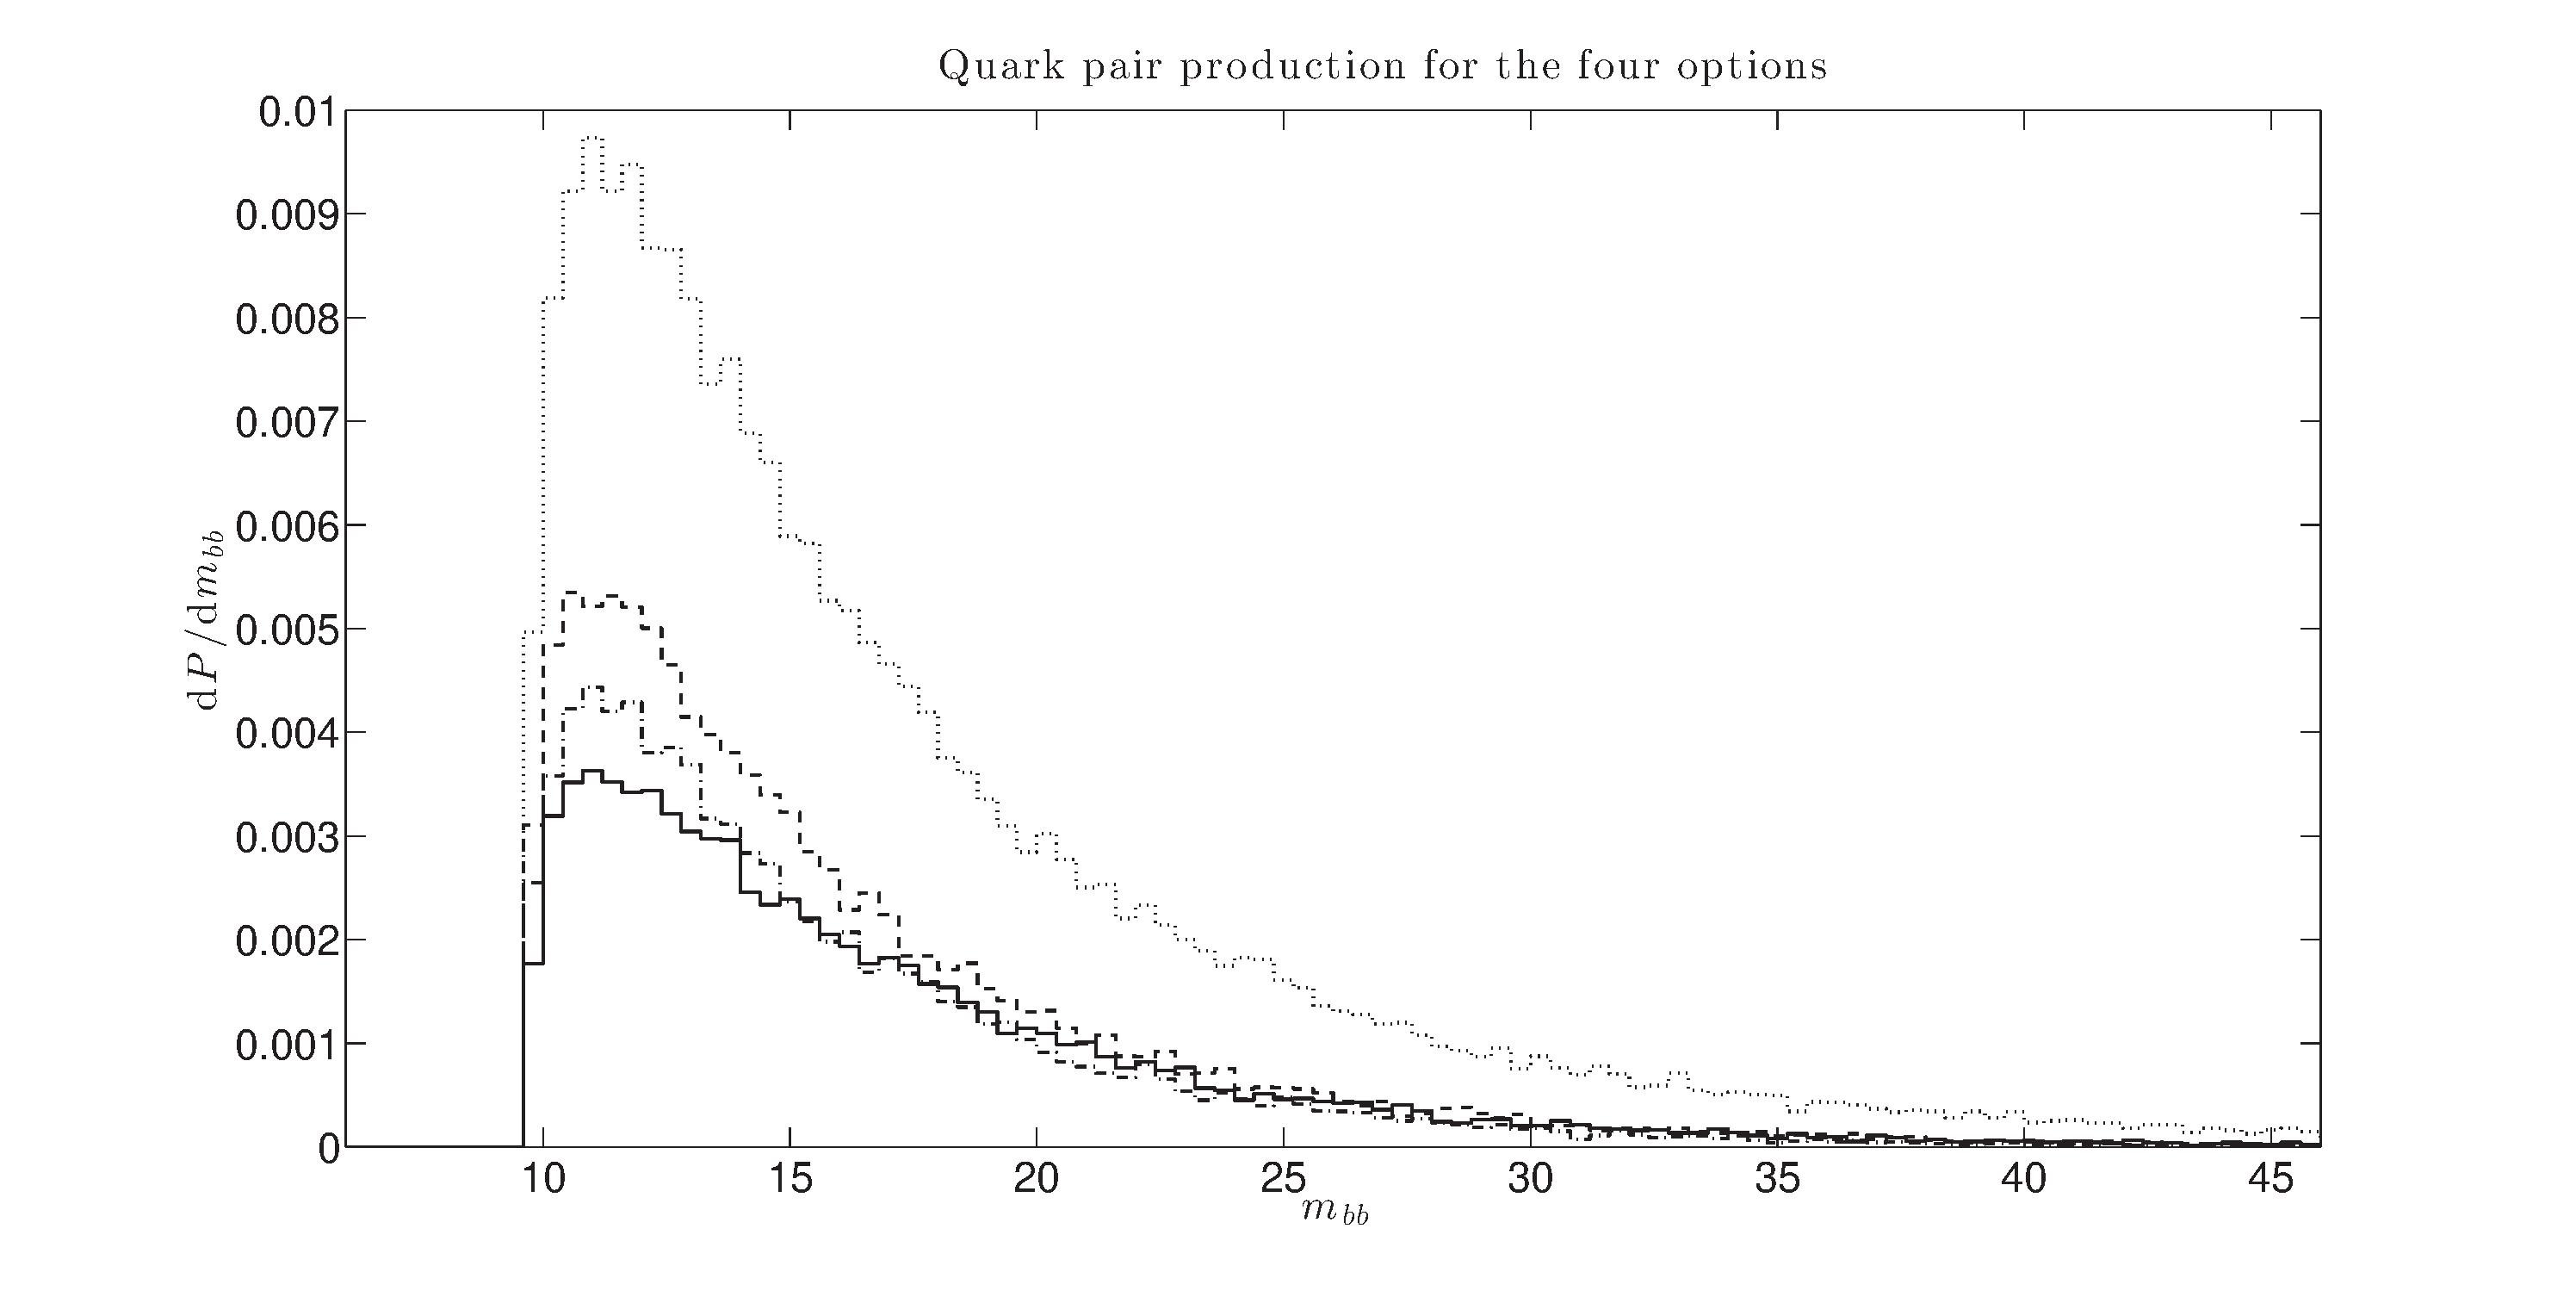
\includegraphics[width=15cm]{QMass}
\label{fig:QMass}
\end{figure}



Las características importantes de las opciones 1-4, discutidas en \ref{subsubsec:PythiaAlg}, están presentes en este gráfico. La opción 3 representa el caso extremo. La compensación entre el acrecentamiento en la zona umbral y la supresión a masas altas es visible para la opción 4. Esta compensación corrige el valor de la tasa total (área bajo la curva) a un valor similar al dado por la opción 1. En principio, no hay ninguna razón para esperar que estos dos efectos se compensaran tan cercanamente en la tasa total. La opción 2 presenta una producción visiblemente mayor que la opción 1 en la zona umbral de producción.

Las tasas dadas por las opciones que usan $m^2$ como variable de evolución (5-8) conllevan a una tasa ligeramente menor que las dadas por las primeras 4 opciones, alrededor de 5\% menos.

Los valores dados por las opciones 1, 4, 5, 6 y 8 caen dentro del error total de las últimas tres referencias en la tabla \ref{table:gbbMeasurements}. El valor dado por la opción 2 está por poco fuera de los errores, pero aún dentro de dos desviaciones estándar. Las opciones 3 y 7 no parecieran resproducir los datos experimentales, ya que se encuentran lejanamente fuera del límite superior indicado por todas las mediciones.

Las discrepancias pueden estar relacionadas a la masa desnuda del quark bottom, una cantidad que no puede ser medida directamente. Usando una masa $m_\b$ más alta que la dada por defecto, las tasas simuladas se reducirían, acercándose más a los resultados experimentales. Además, tomando en cuenta los errores sistemáticos mostrados en la tabla \ref{table:gbbMeasurements} y la dispersión de los valores, podemos notar que se trata de una medición complicada.

\subsection{El espectro de la fracción de energía de los mesones $\D^{*\pm}$}

Vamos a estudiar ahora la producción de mesones $\D^{*\pm}$ como función de la fracción de energía $X_E$. La colaboración ALEPH tiene mediciones para esto en \cite{Barate:1999bg}. El espectro total es tomado como la suma de tres componentes: mesones provenientes de charms primarios, de bottoms primarios y de quarks pesados secundarios, es decir, provenientes de ramificaciones a partir de gluones.

\begin{figure}[h]
\centering
\caption[Espectro de la fracción de energía de los mesones $\D^{*\pm}$.]{Distribución de la fracción de energía para los mesones  $\D^{*\pm}$. Los puntos con barras de error son las mediciones de ALEPH  y la línea sólida corresponde a la simulación de \textsc{Pythia}, con las contribuciones correspondientes de: $\b\bbar$ (puntos), $\c\cbar$ (líneas) y ramificaciones de gluón (líneas y puntos).}
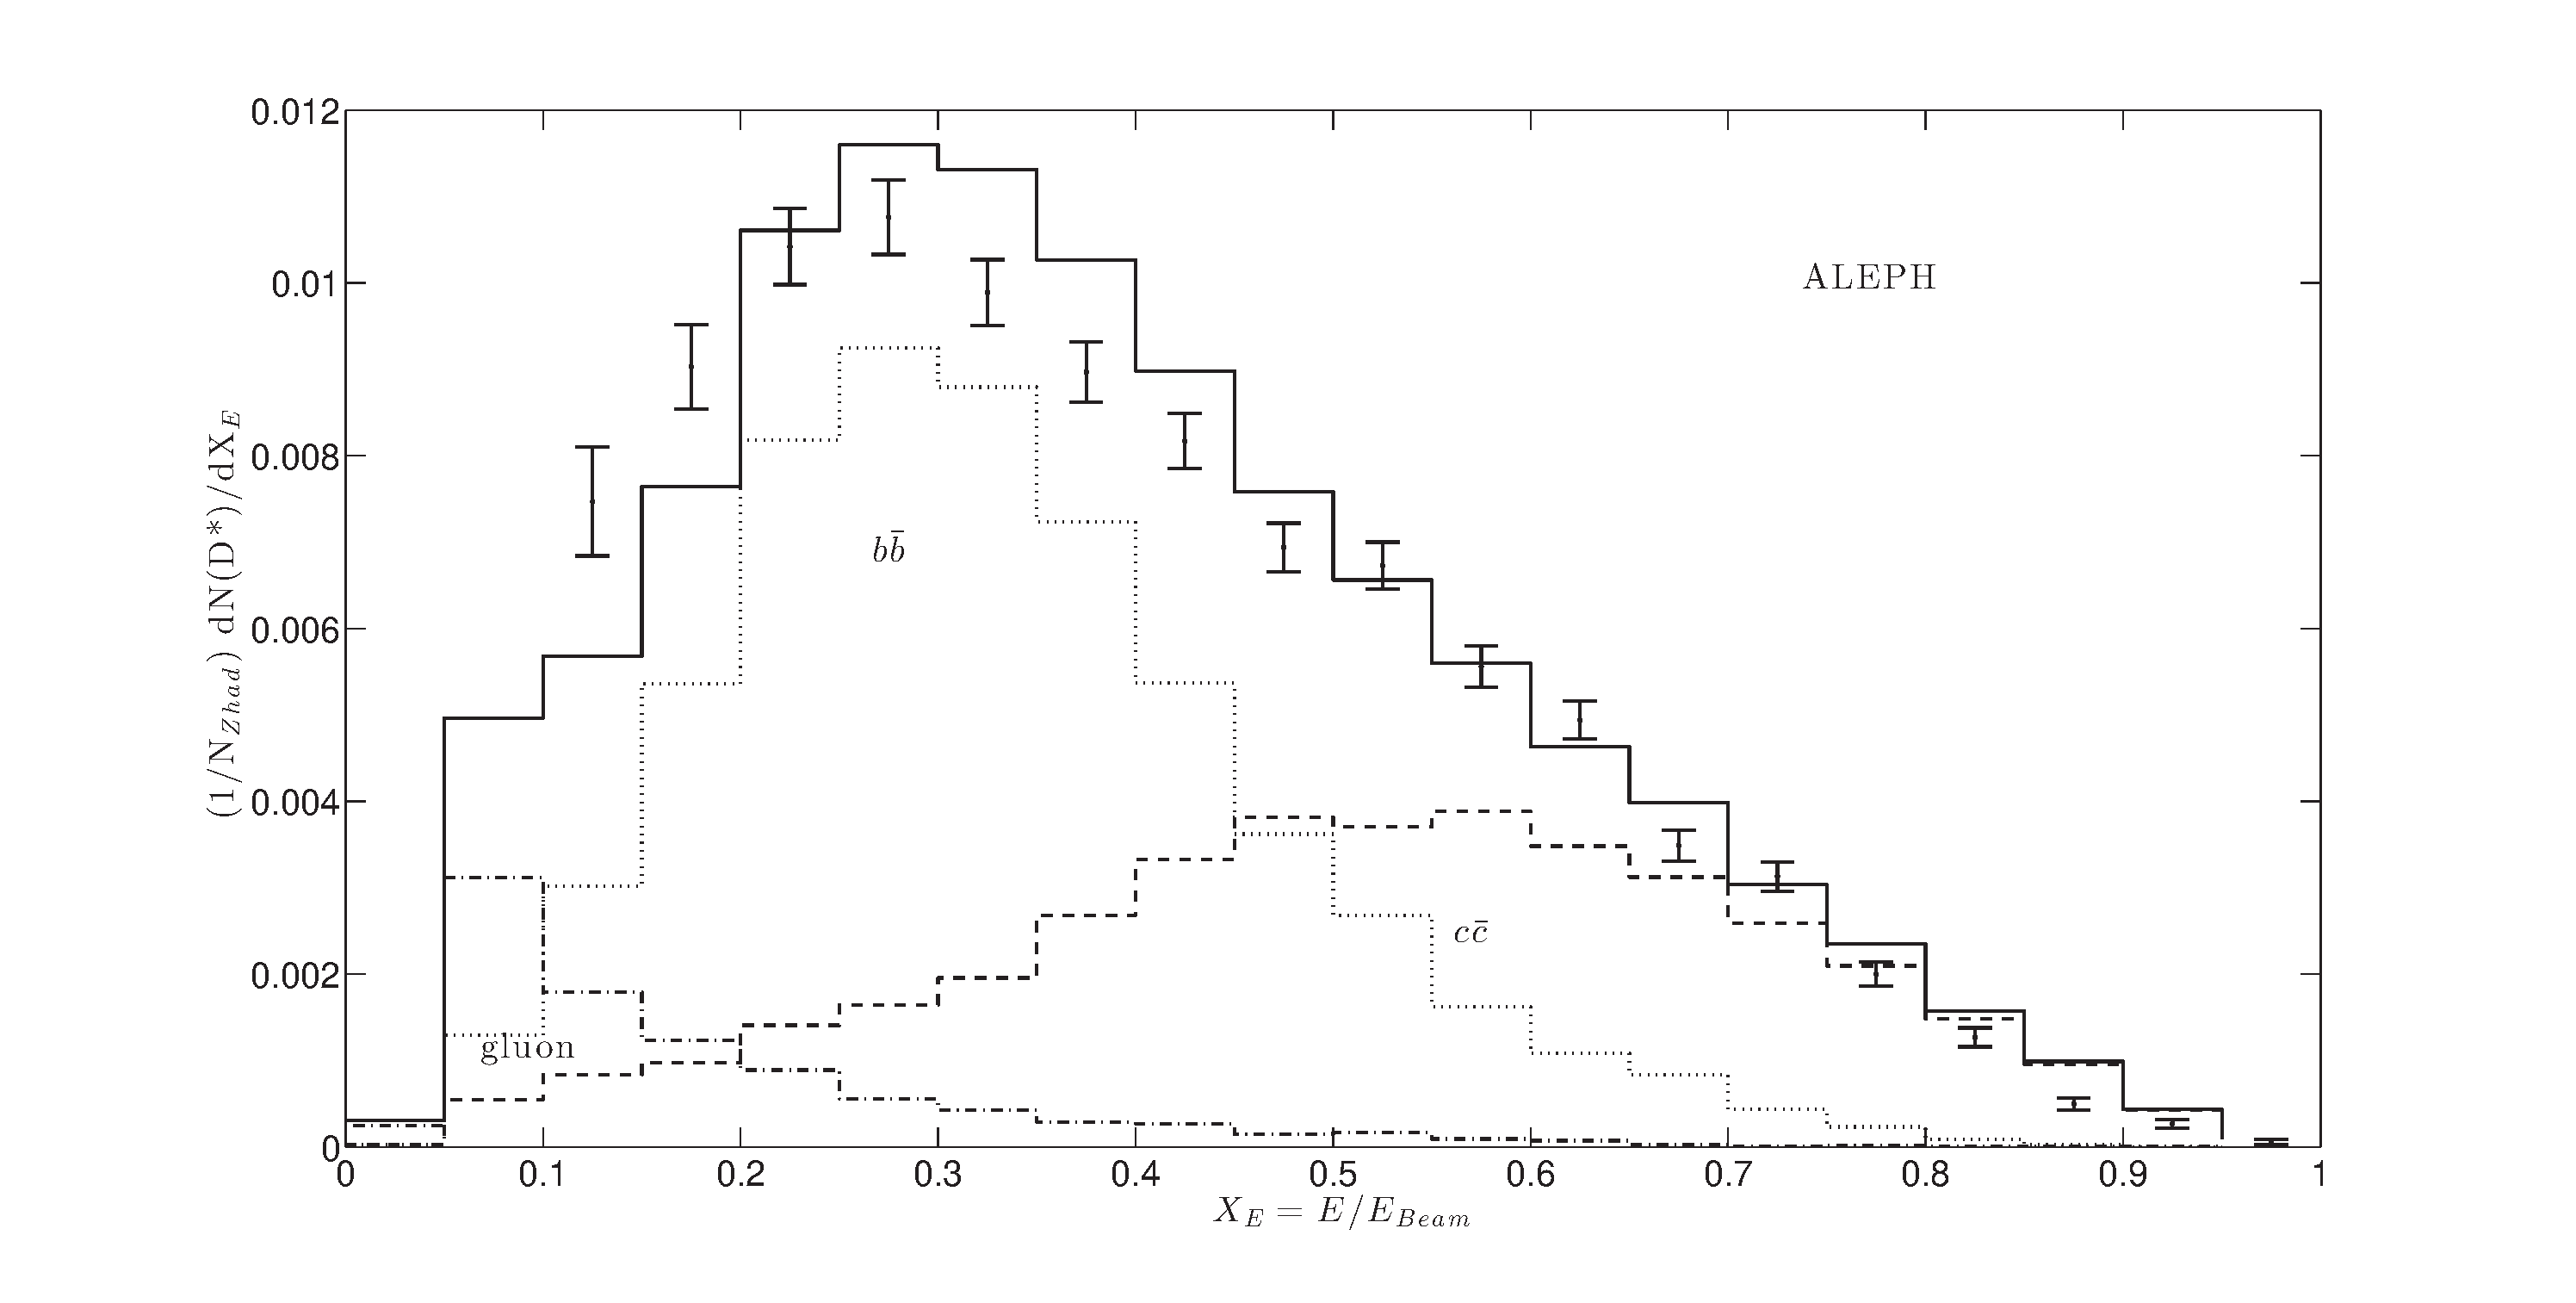
\includegraphics[width=15cm]{DStarOp1Thesis}
\label{fig:ALEPHPythia1}
\end{figure}



En gráfico en la figura \ref{fig:ALEPHPythia1} muestra que las mediciones de ALEPH y la simulación de \textsc{Pythia} (opción 1) con sus componentes. Podemos ver que la contribución principal de la ramificación de gluones sucede a fracciones de energía bajas, lo que se debe al hecho de que los quarks secundarios son producidos al menos en una tercera ramificación, partiendo desde el $Z^0$ (como en la figura \ref{fig:PrimSecQuarks}), cuando ya la energía ha sido distribuída en varios productos. De este modo, el impacto de las opciones será a fracciones de energía bajas. La figura también sugiere la necesidad de una corrección a energías bajas, incluso para las contribuciones de $\b\bbar$ y $\c\cbar$ primarios. Además, la simulación presenta un exceso justo después del pico cercano a $0.3$. Para valores medianos y altos de $X_E$, la simulación y los experimentos concuerdan en buena medida.

La figura \ref{fig:GluonDStar} muestra los casos extremos para la contribución de gluones: opciones 1 y 3. La última presenta valores al menos dos veces mayores que la primera en cada casilla del histograma. Las distribuciones para las opciones 2 y 4 (que no se muestran) dan valores intermedios.

\begin{figure}[h]
\centering
\caption[Contribución de los gluones a la producción de $\D^{*\pm}$ en dos casos extremos.]{Casos extremos de la producción de $\D^{*}$ a partir de gluones. Opciones de \textsc{Pythia} 1 (sólida) y 3 (punteada).}
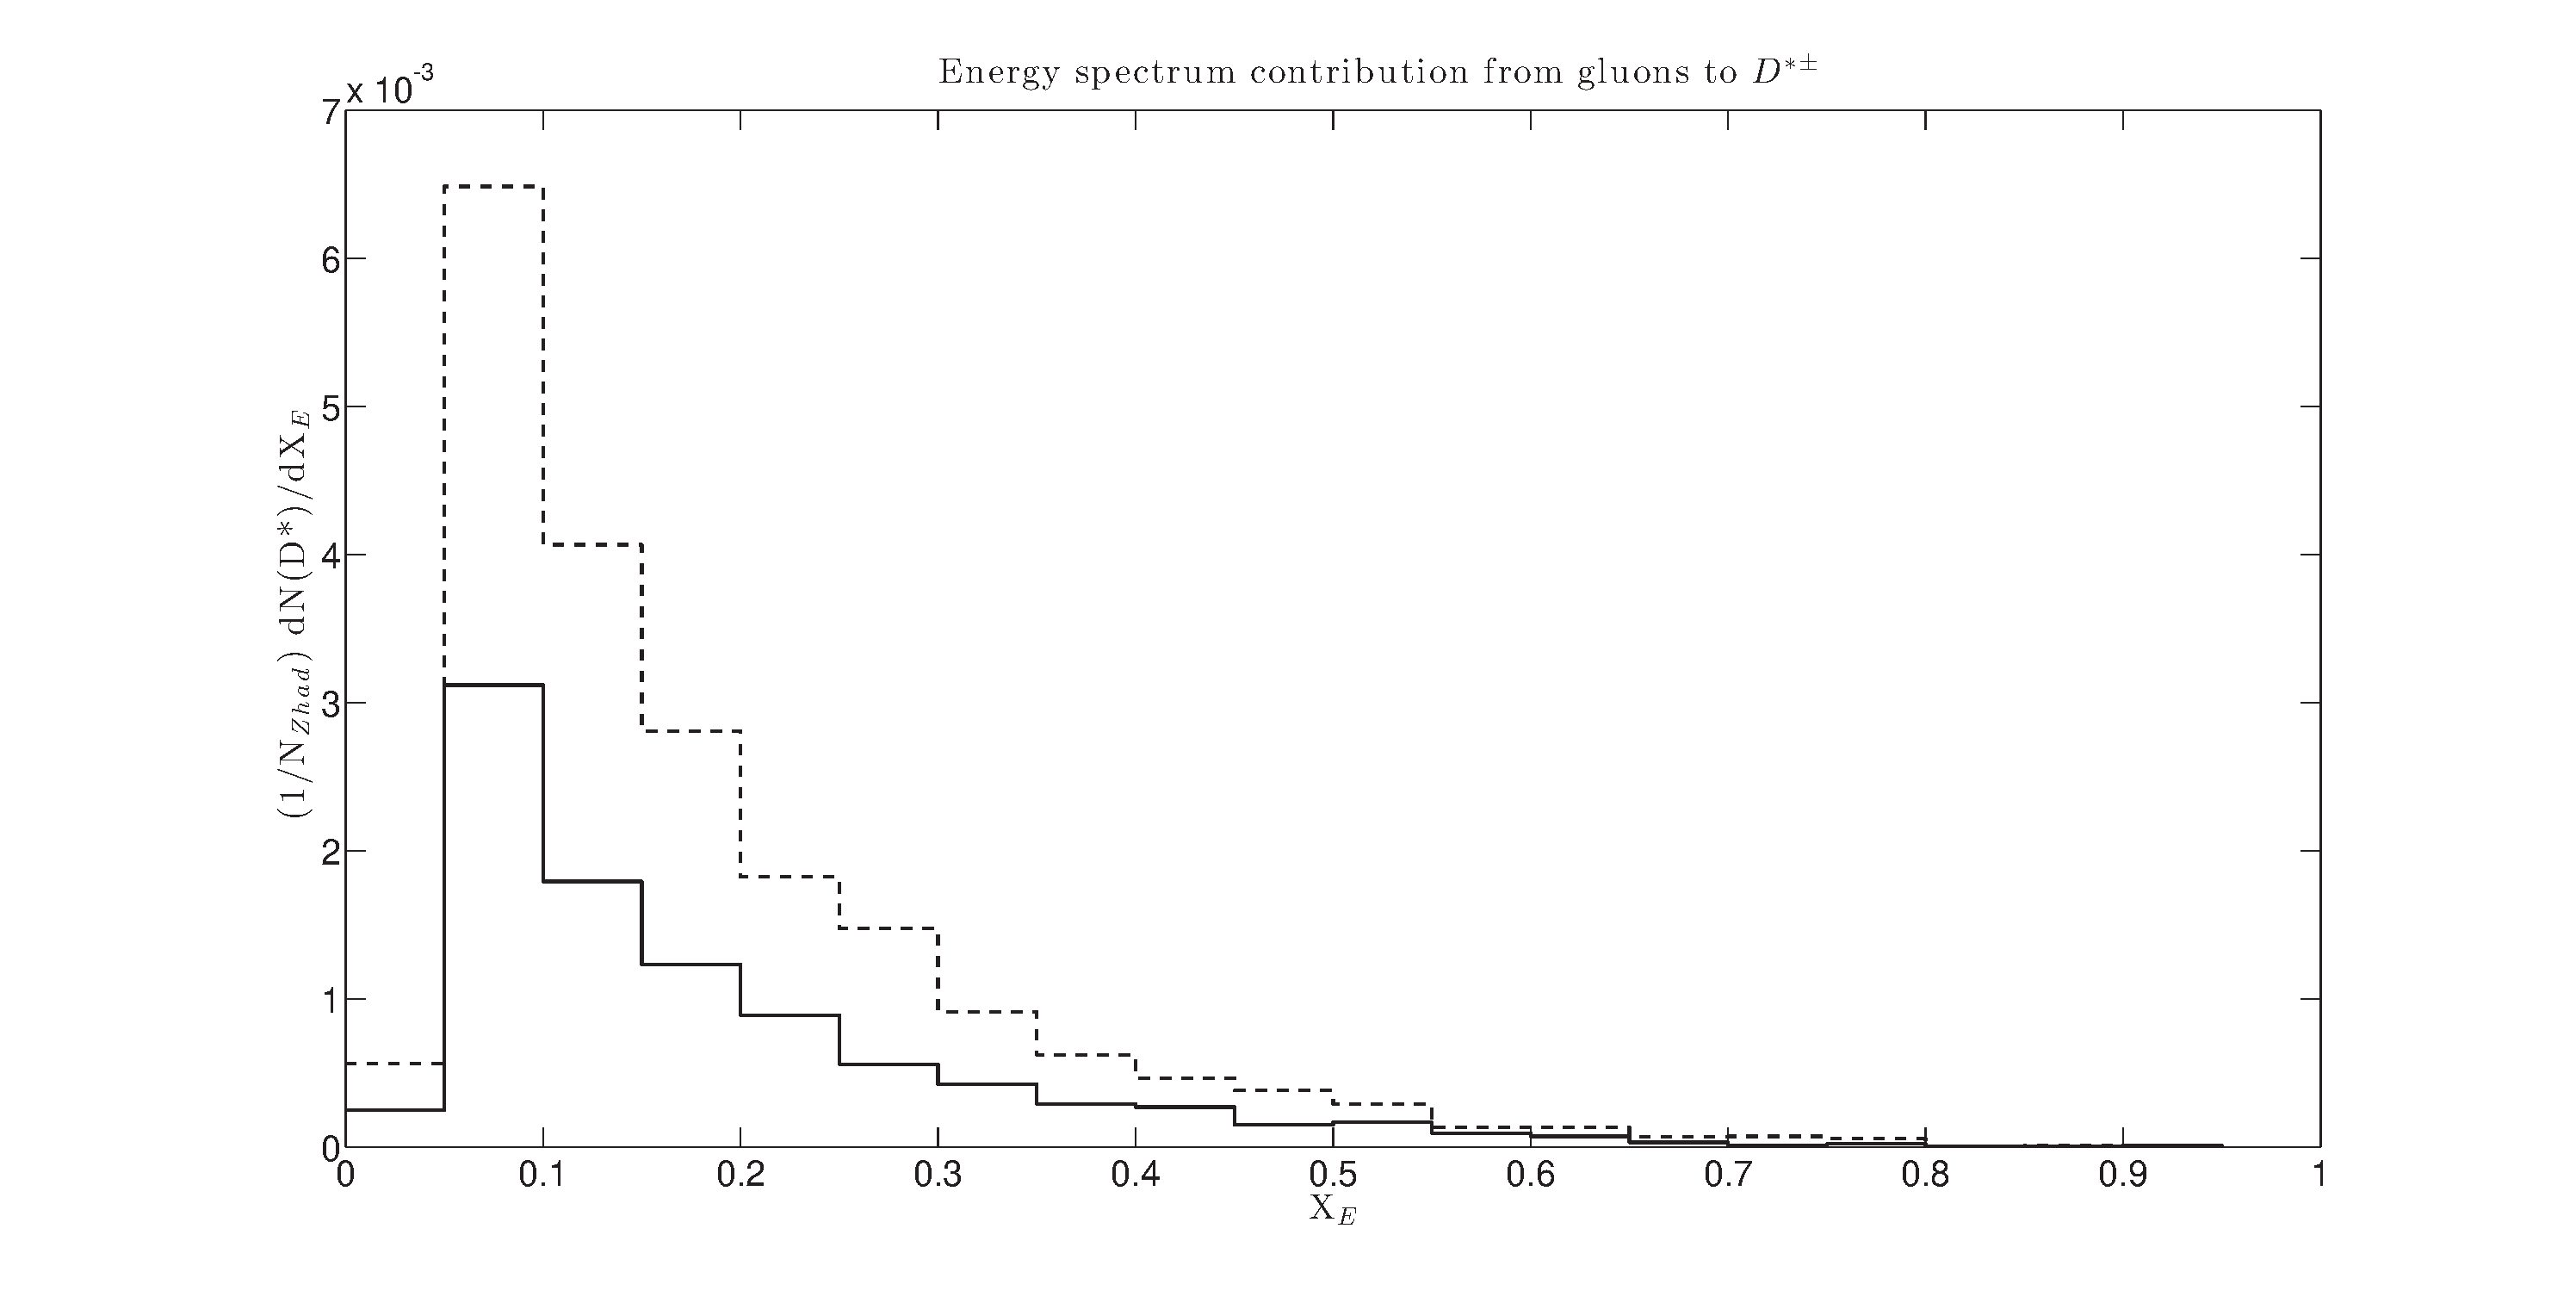
\includegraphics[width=15cm]{GluonDStarThesis}
\label{fig:GluonDStar}
\end{figure}

Para comparar las cuatro opciones con los datos experimentales, la figura \ref{fig:DStarOp} muestra las distribuciones completas y las mediciones de ALEPH. El aumento de producción a bajas energías es evidente para las opciones que no son por defecto, donde las simulaciones se acercan más a los valores experimentales. El exceso cercano al pico está todavía presente y ligeramente aumentado. A altas energías, el decaimiento no muestra diferencias significativas con respecto a la opción por defecto (debido a que en esta zona la contribución secundaria es despreciable) y siguen aproximadamente el comportamiento de los datos.

\begin{figure}[!h]
\centering
\caption[Espectro de la fracción de energía de $\D^{*\pm}$. Simulación y datos comparados.]{Espectro de la fracción de energía de $\D^{*\pm}$. Datos de ALEPH (puntos con barras de error) y las opciones de \textsc{Pythia}: por defecto (sólida), 2 (puntos), 3 (líneas) y 4 (líneas y puntos).}
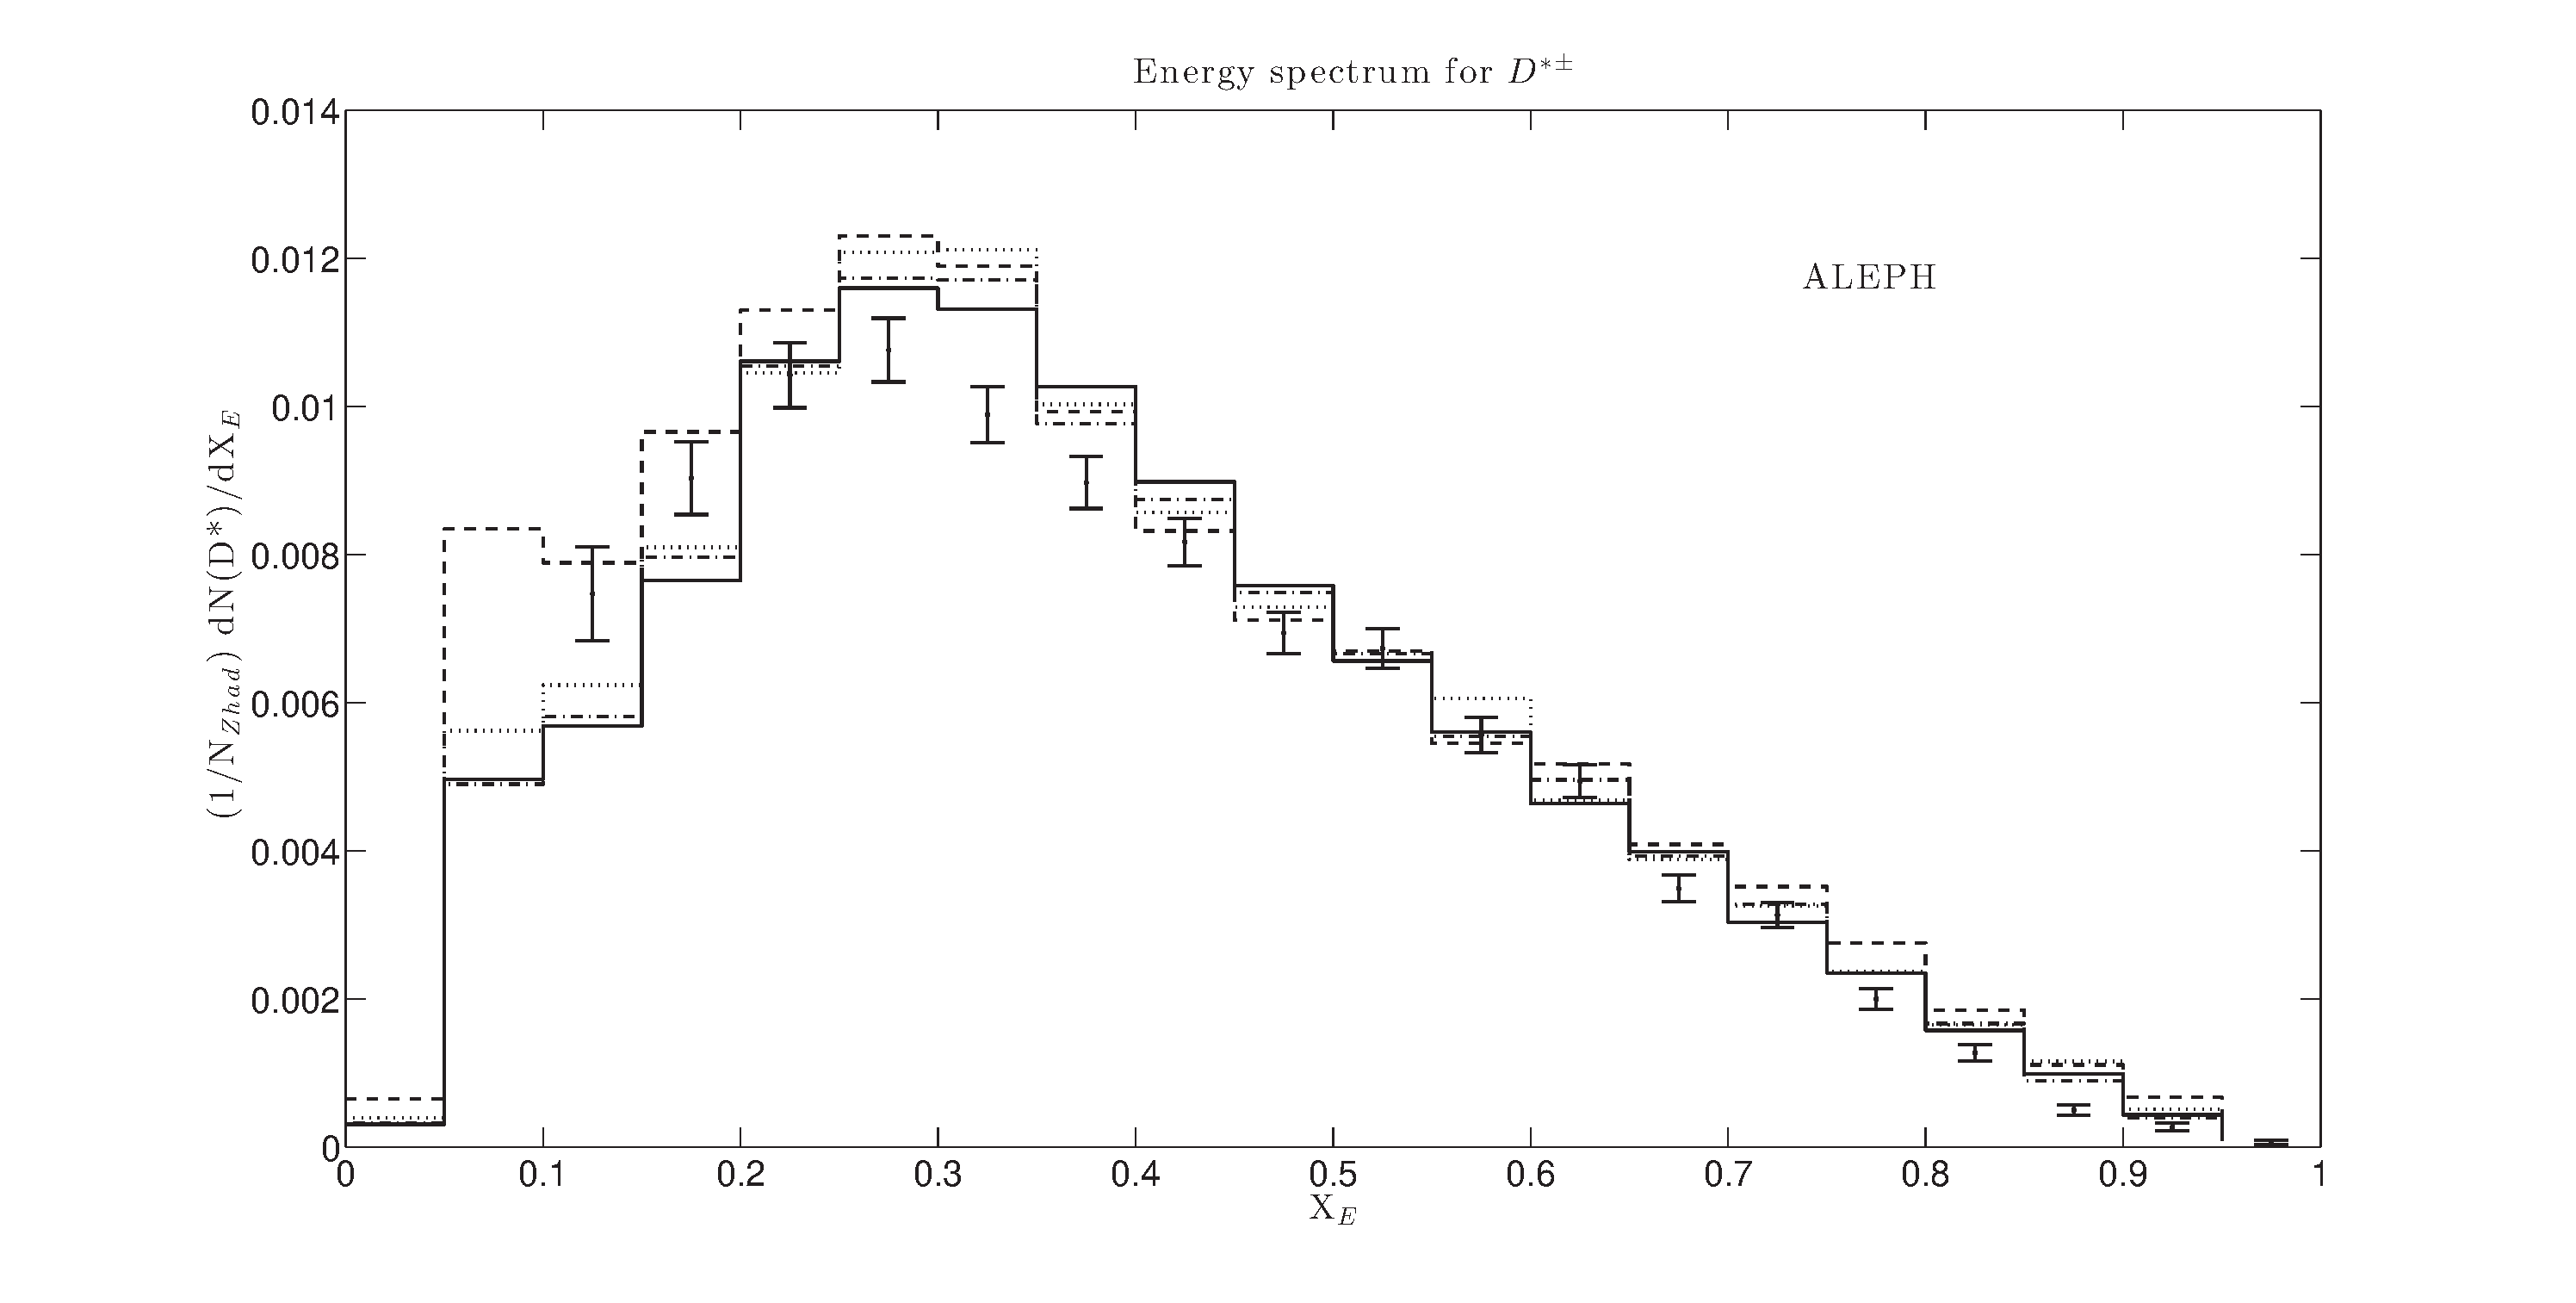
\includegraphics[width=15cm]{DStarOpThesis}
\label{fig:DStarOp}
\end{figure}

En este contexto, la opción 3 parece un buen candidato, debido a que corrige (con algo de precisión) la producción de mesones $\D^*$ a bajas energías. Para la región justo después del pico, el aumento puede ser mayor al deseado, pero aún así los datos en su totalidad son más cercanos a esta opción.

Debido a su carácter no-perturbativo, el decaimiento de mesones es un fenómeno que no se entiende completamente. Un modelado algo diferente del decaimiento $\B\to D$ pudiera correr algunos eventos después del pico a más bajas energías, para ajustarse mejor a los datos experimentales en ambas regiones, sin requerir una tasa $\g\to\b\bbar$ mayor. De esta manera, este estudio no puede concluir definitivamente sobre esta desviación.

\section{Colisiones protón-protón a 7000 GeV}

Tornando ahora al tema de las colisiones hadrónicas, estudiaremos las correlaciones entre pares de hadrones $\B$. Eventos con un par son clasificados de acuerdo a PC, FE y GS. Eventos con más pares son clasificados como mezclados.

Una simulación de $5\times10^6$ eventos fue llevada a cabo para cada opción. Fueron seleccionados para el análisis eventos con dos mesones $\B$, cada uno con un momentum transverso mayor a 15 GeV. Un corte inferior para el momentum transverso del proceso duro de 15 GeV también fue impuesto; este criterio es necesario debido a que eventos con $\pT$ más bajo son producidos en mayor cantidad, pero el número de eventos seleccionados decrece para valores menores de 20 GeV, como se puede ver en la figura \ref{fig:accepted}. Allí, sólo alrededor del 1\% de los eventos son seleccionados para el análisis. Un corte aún más bajo incrementaría tal ``ineficiencia'', seleccionando sólo unos pocos más eventos en comparación con el total generado.

\begin{figure}[h]
\centering
\caption[Eventos generados y aceptados en colisiones hadrónicas.]{Eventos generados (sólida) y aceptados (punteada) como función del momentum transverso del proceso.}
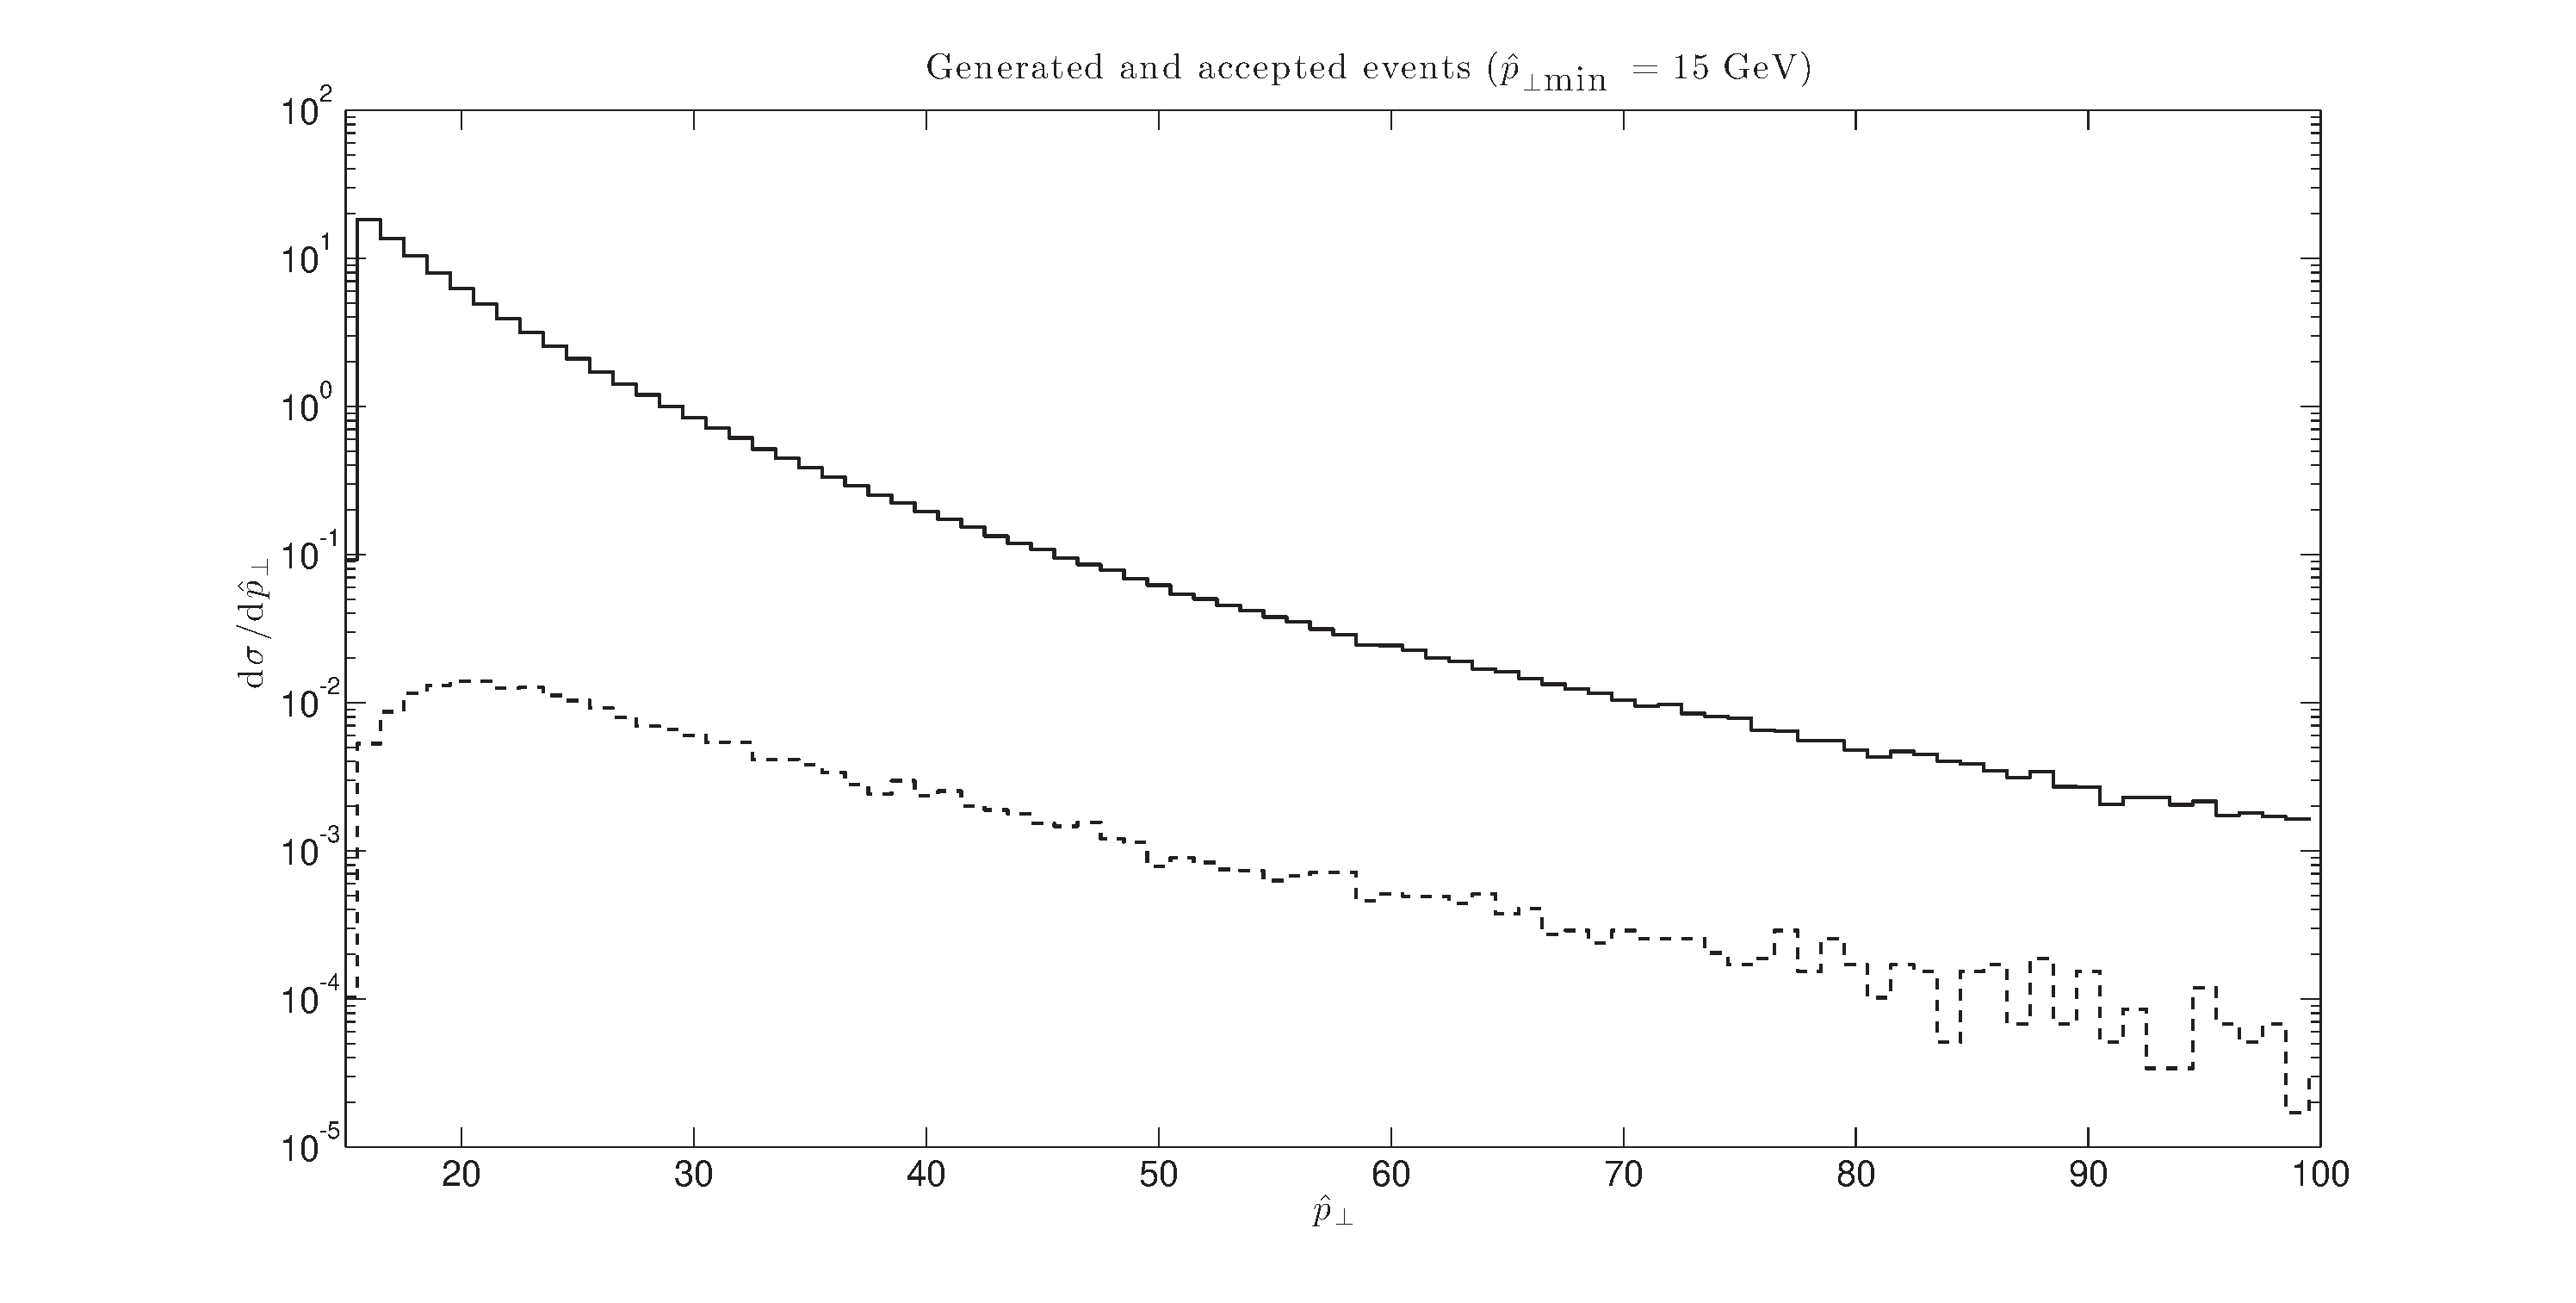
\includegraphics[width=15cm]{Accepted}
\label{fig:accepted}
\end{figure}

\subsection{Separaciones azimutales angulares}

La variación del ángulo azimutal es una buena medida de la separación de dos mesones $\B$, debido a que es un invariante de Lorentz bajo boosts a lo largo del eje de colisión ($z$). La diferencia $\Delta \varphi$  es medida en el plano perpendicular al eje $z$. La figura \ref{fig:BBPhiOp1}  muestra la producción de pares de mesones bottom en términos de la separación angular azimutal, para la opción 1.

\begin{figure}[!h]
\centering
\caption[Separación angular azimutal de pares de mesones $\B$. Opción por defecto de \textsc{Pythia}.]{Separación angular azimutal de pares de mesones $\B$ usando la opción por defecto de \textsc{Pythia} incluyendo las cuatro fuentes de producción.}
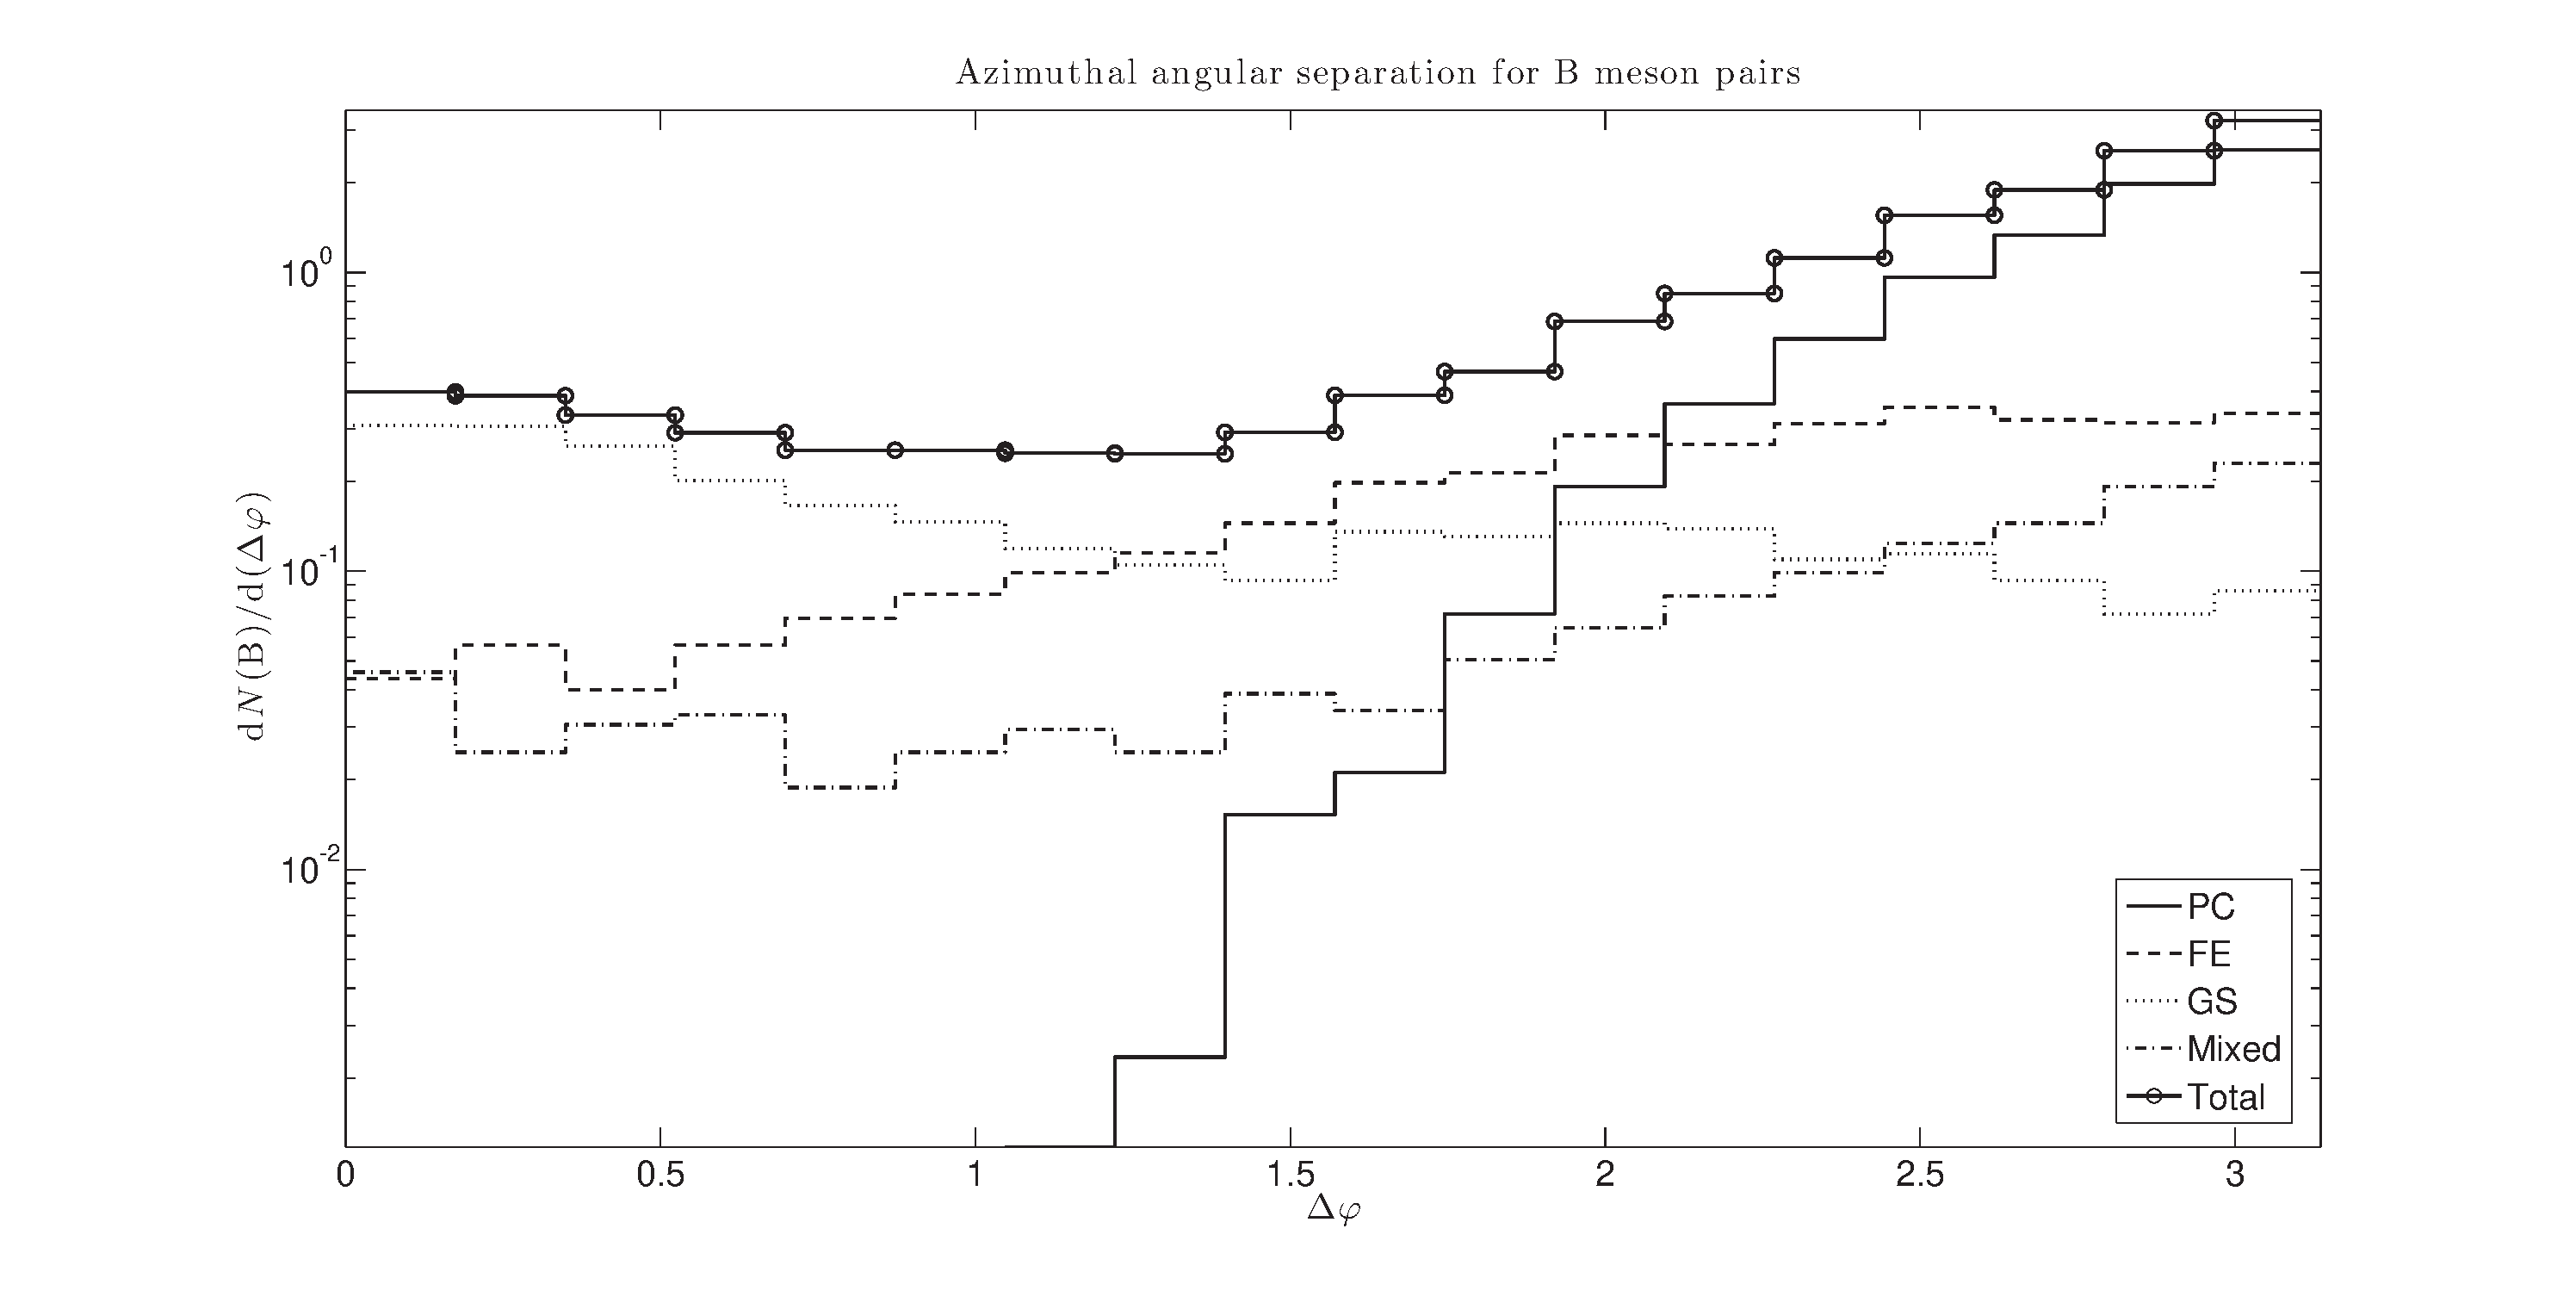
\includegraphics[width=15cm]{BBPhiOp1}
\label{fig:BBPhiOp1}
\end{figure}
Varios rasgos de las correlaciones en los mecanismos de producción son visibles: PC muestra un pico a ángulos altos, debido a que los pares son creados en el proceso duro y tienden a producir quarks en sentidos opuestos, mientras que GS contribuye mayormente en la región de poca abertura. Pares creados a partir de FE están menos anticorrelacionados que los provenientes de PC. Los mesones $\B$ mezclados muestran una distribución angular homogénea, ya que no hay una relación particular entre los mesones provenientes de ramificaciones de gluones distintas.

La variación de las opciones de \textsc{Pythia} es mostrada en la figura \ref{fig:BBPhi4Op}.

\begin{figure}[!h]
\centering
\caption[Separación angular de pares de mesones $\B$. Cuatro opciones de \textsc{Pythia}.]{Separación angular azimutal de pares de mesones $\B$ usando las opciones de \textsc{Pythia} 1 (sólida), 2 (líneas), 3 (puntos) y 4 (líneas y puntos).}
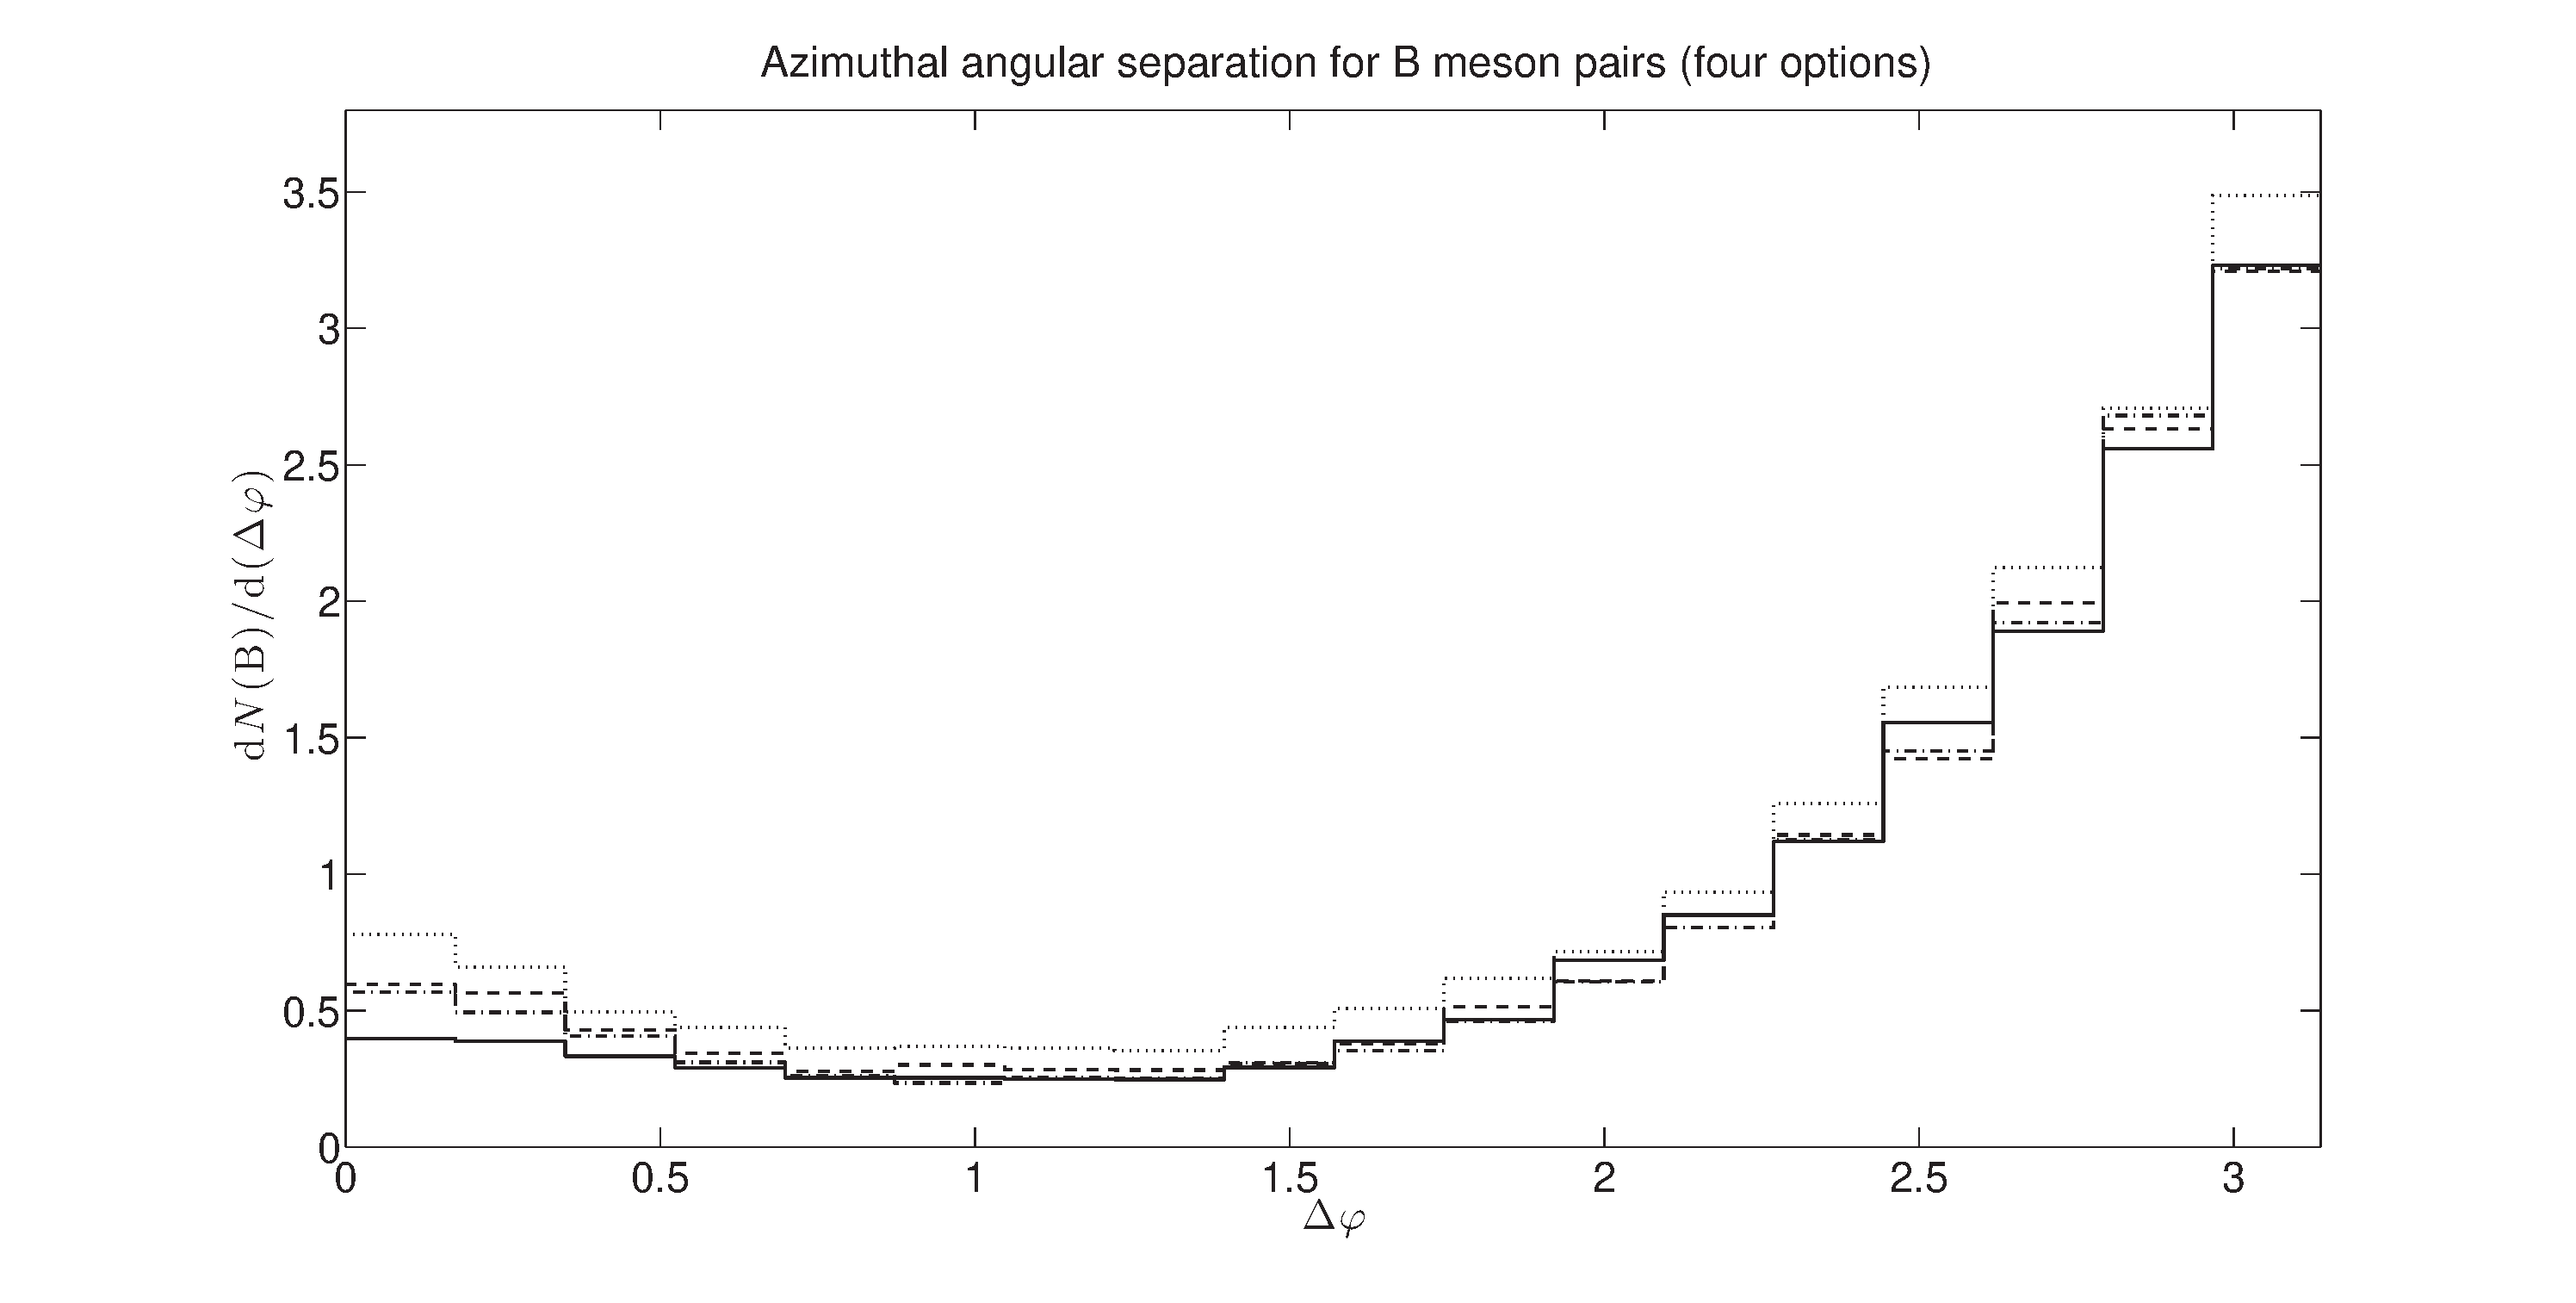
\includegraphics[width=15cm]{BBPhi4Op}
\label{fig:BBPhi4Op}
\end{figure}
De manera similar al caso discutido en la sección previa, los dos casos extremos (superior e inferior) a ángulos azimutales bajos están dados por la opciones 3 y 1, donde la ramificación de gluones es dominante. Las opciones 2 y 4 son intermedias en esta región.

\subsection{Rapideces relativas}

La rapidez, definida como

$$
y =\frac12 \ln \frac{E+p_z}{E-p_z},
$$
es una medida de la separación de la partícula al eje $z$. De hecho, está relacionada al ángulo polar (entre la partícula y el eje $z$). Se puede mostrar que la diferencia $\Delta y \equiv y_2 - y_1$ es invariante bajo un boost a lo largo del eje $z$.

En gráfico en la figura \ref{fig:BBYOp1} muestra la producción de pares de mesones $\B$ como una función de las rapideces relativas $\Delta y$, simuladas con la opción por defecto de \textsc{Pythia}.

\begin{figure}[!h]
\centering
\caption[Rapidez relativa de pares de mesones $\B$. Opción por defecto de \textsc{Pythia}.]{Rapidez relatica de pares de mesones $\B$ usando la opción por defecto de \textsc{Pythia}, incluyendo la clasificaciónd e las fuentes de producción.}
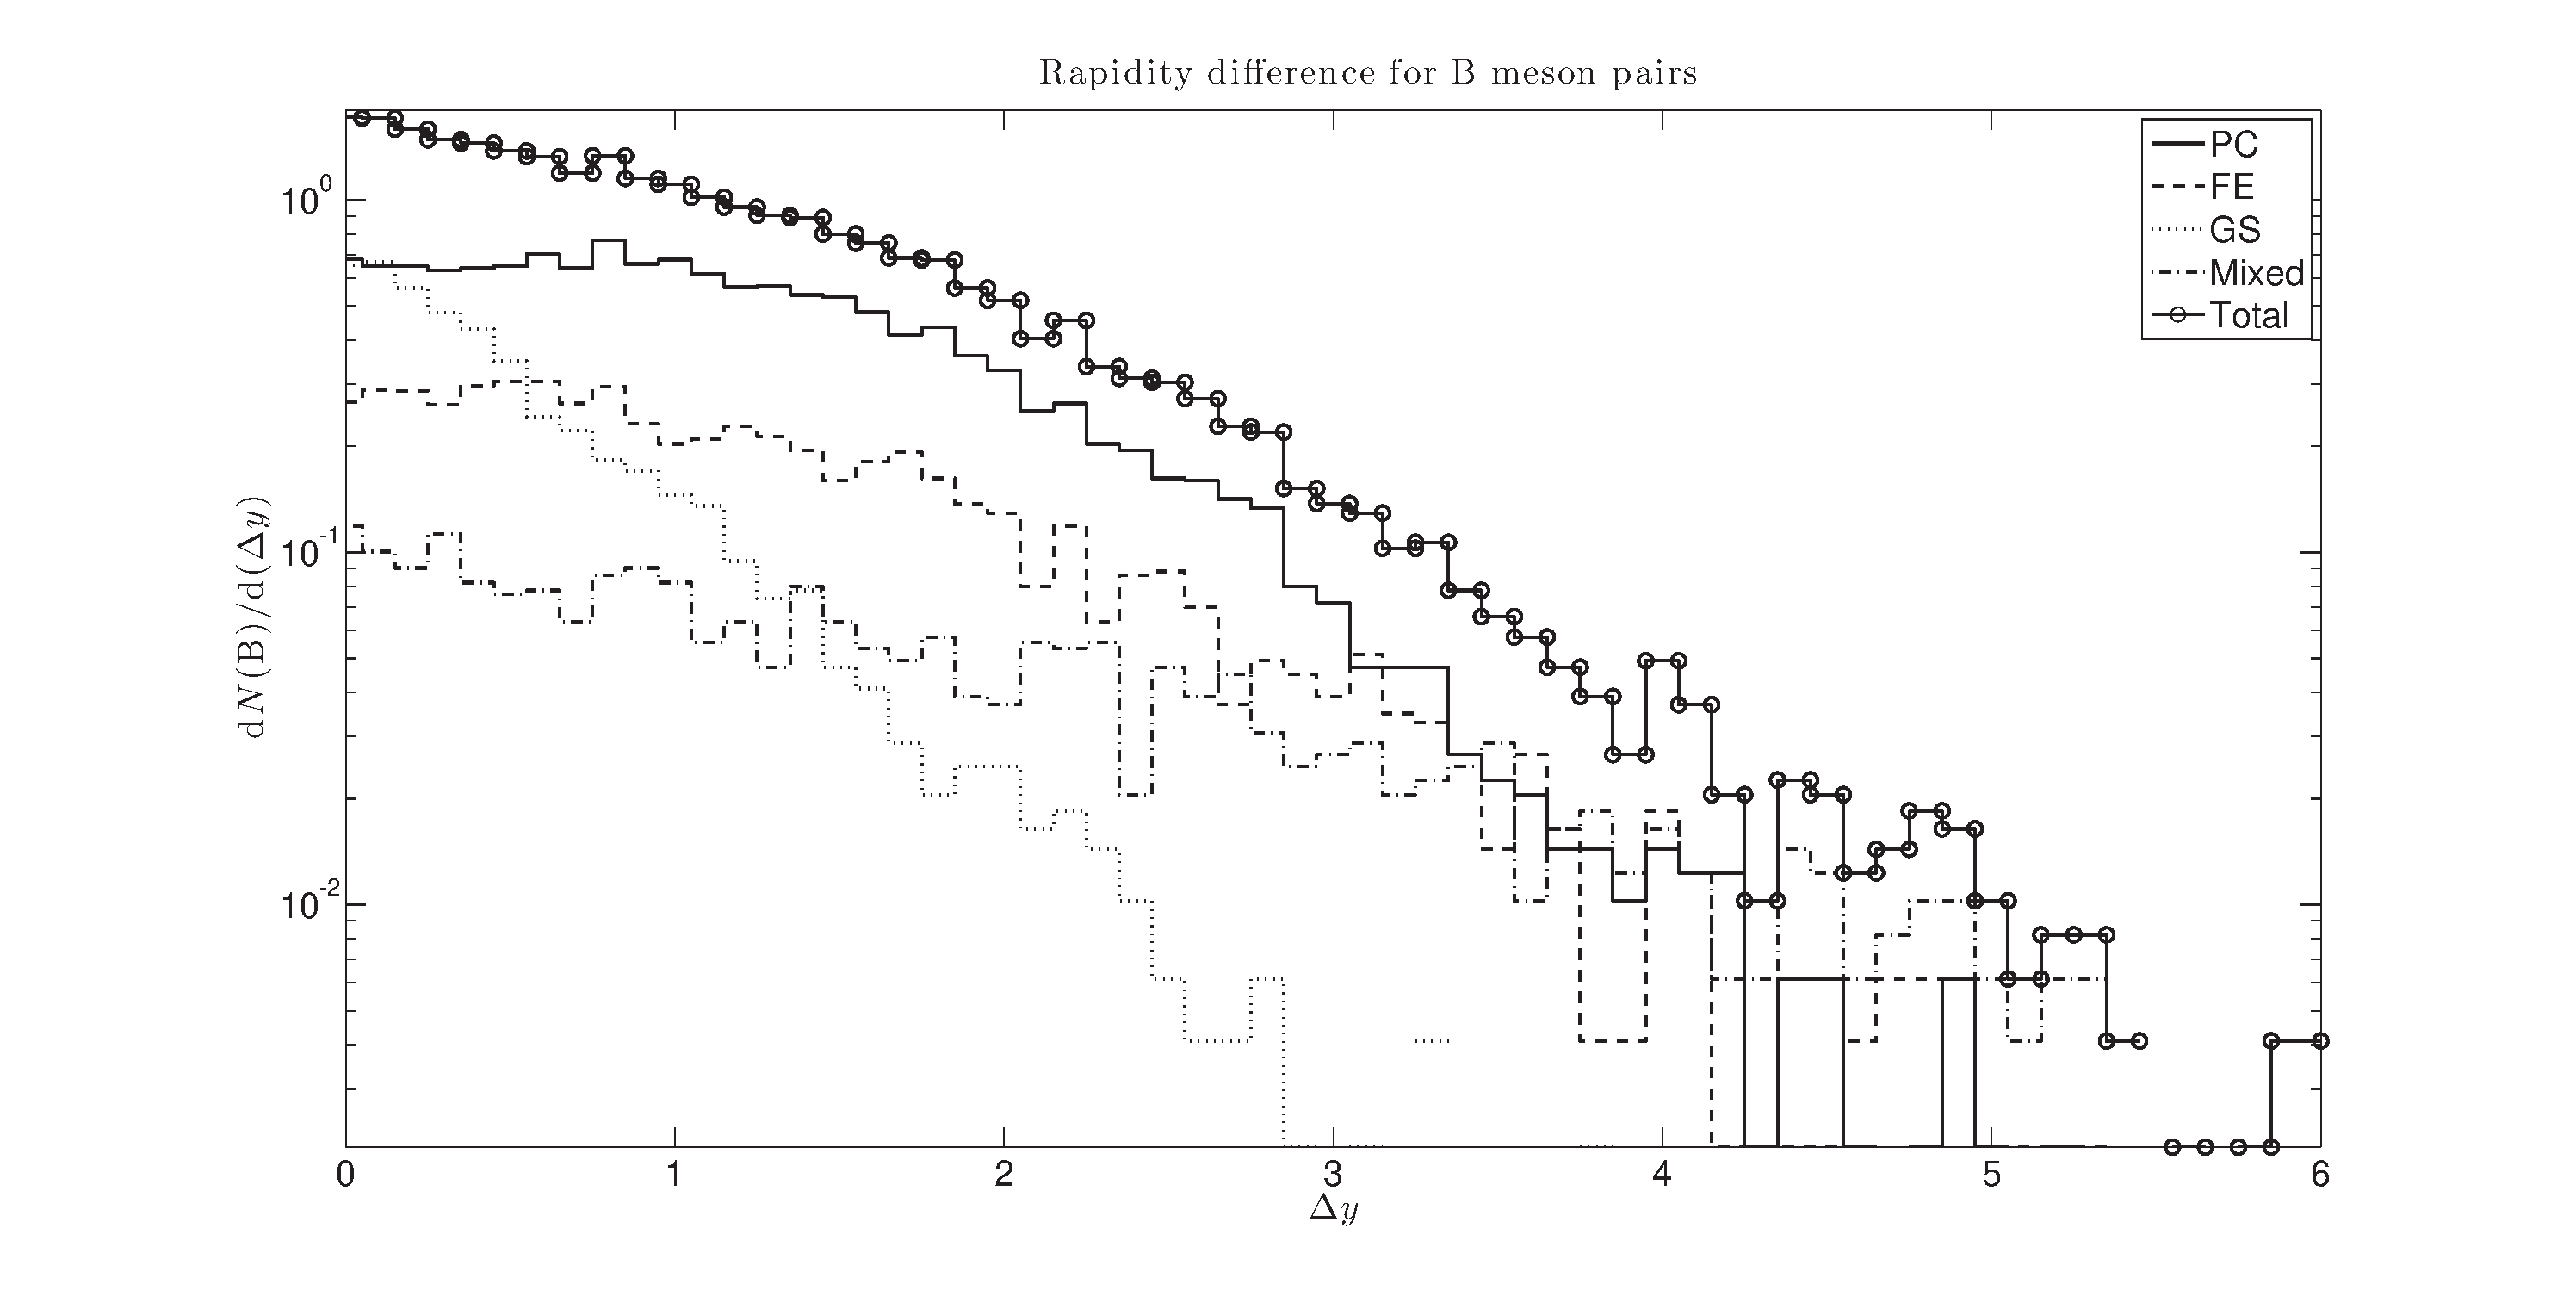
\includegraphics[width=15cm]{BBYOp1}
\label{fig:BBYOp1}
\end{figure}

\begin{figure}[!h]
\centering
\caption[[Rapidez relativa de pares de mesones $\B$. Cuatro opciones de \textsc{Pythia}.]{Rapidez relativa de pares de mesones $\B$ usando la opciones de \textsc{Pythia}:  1 (sólida), 2 (líneas), 3 (puntos) y 4 (líneas y puntos).}
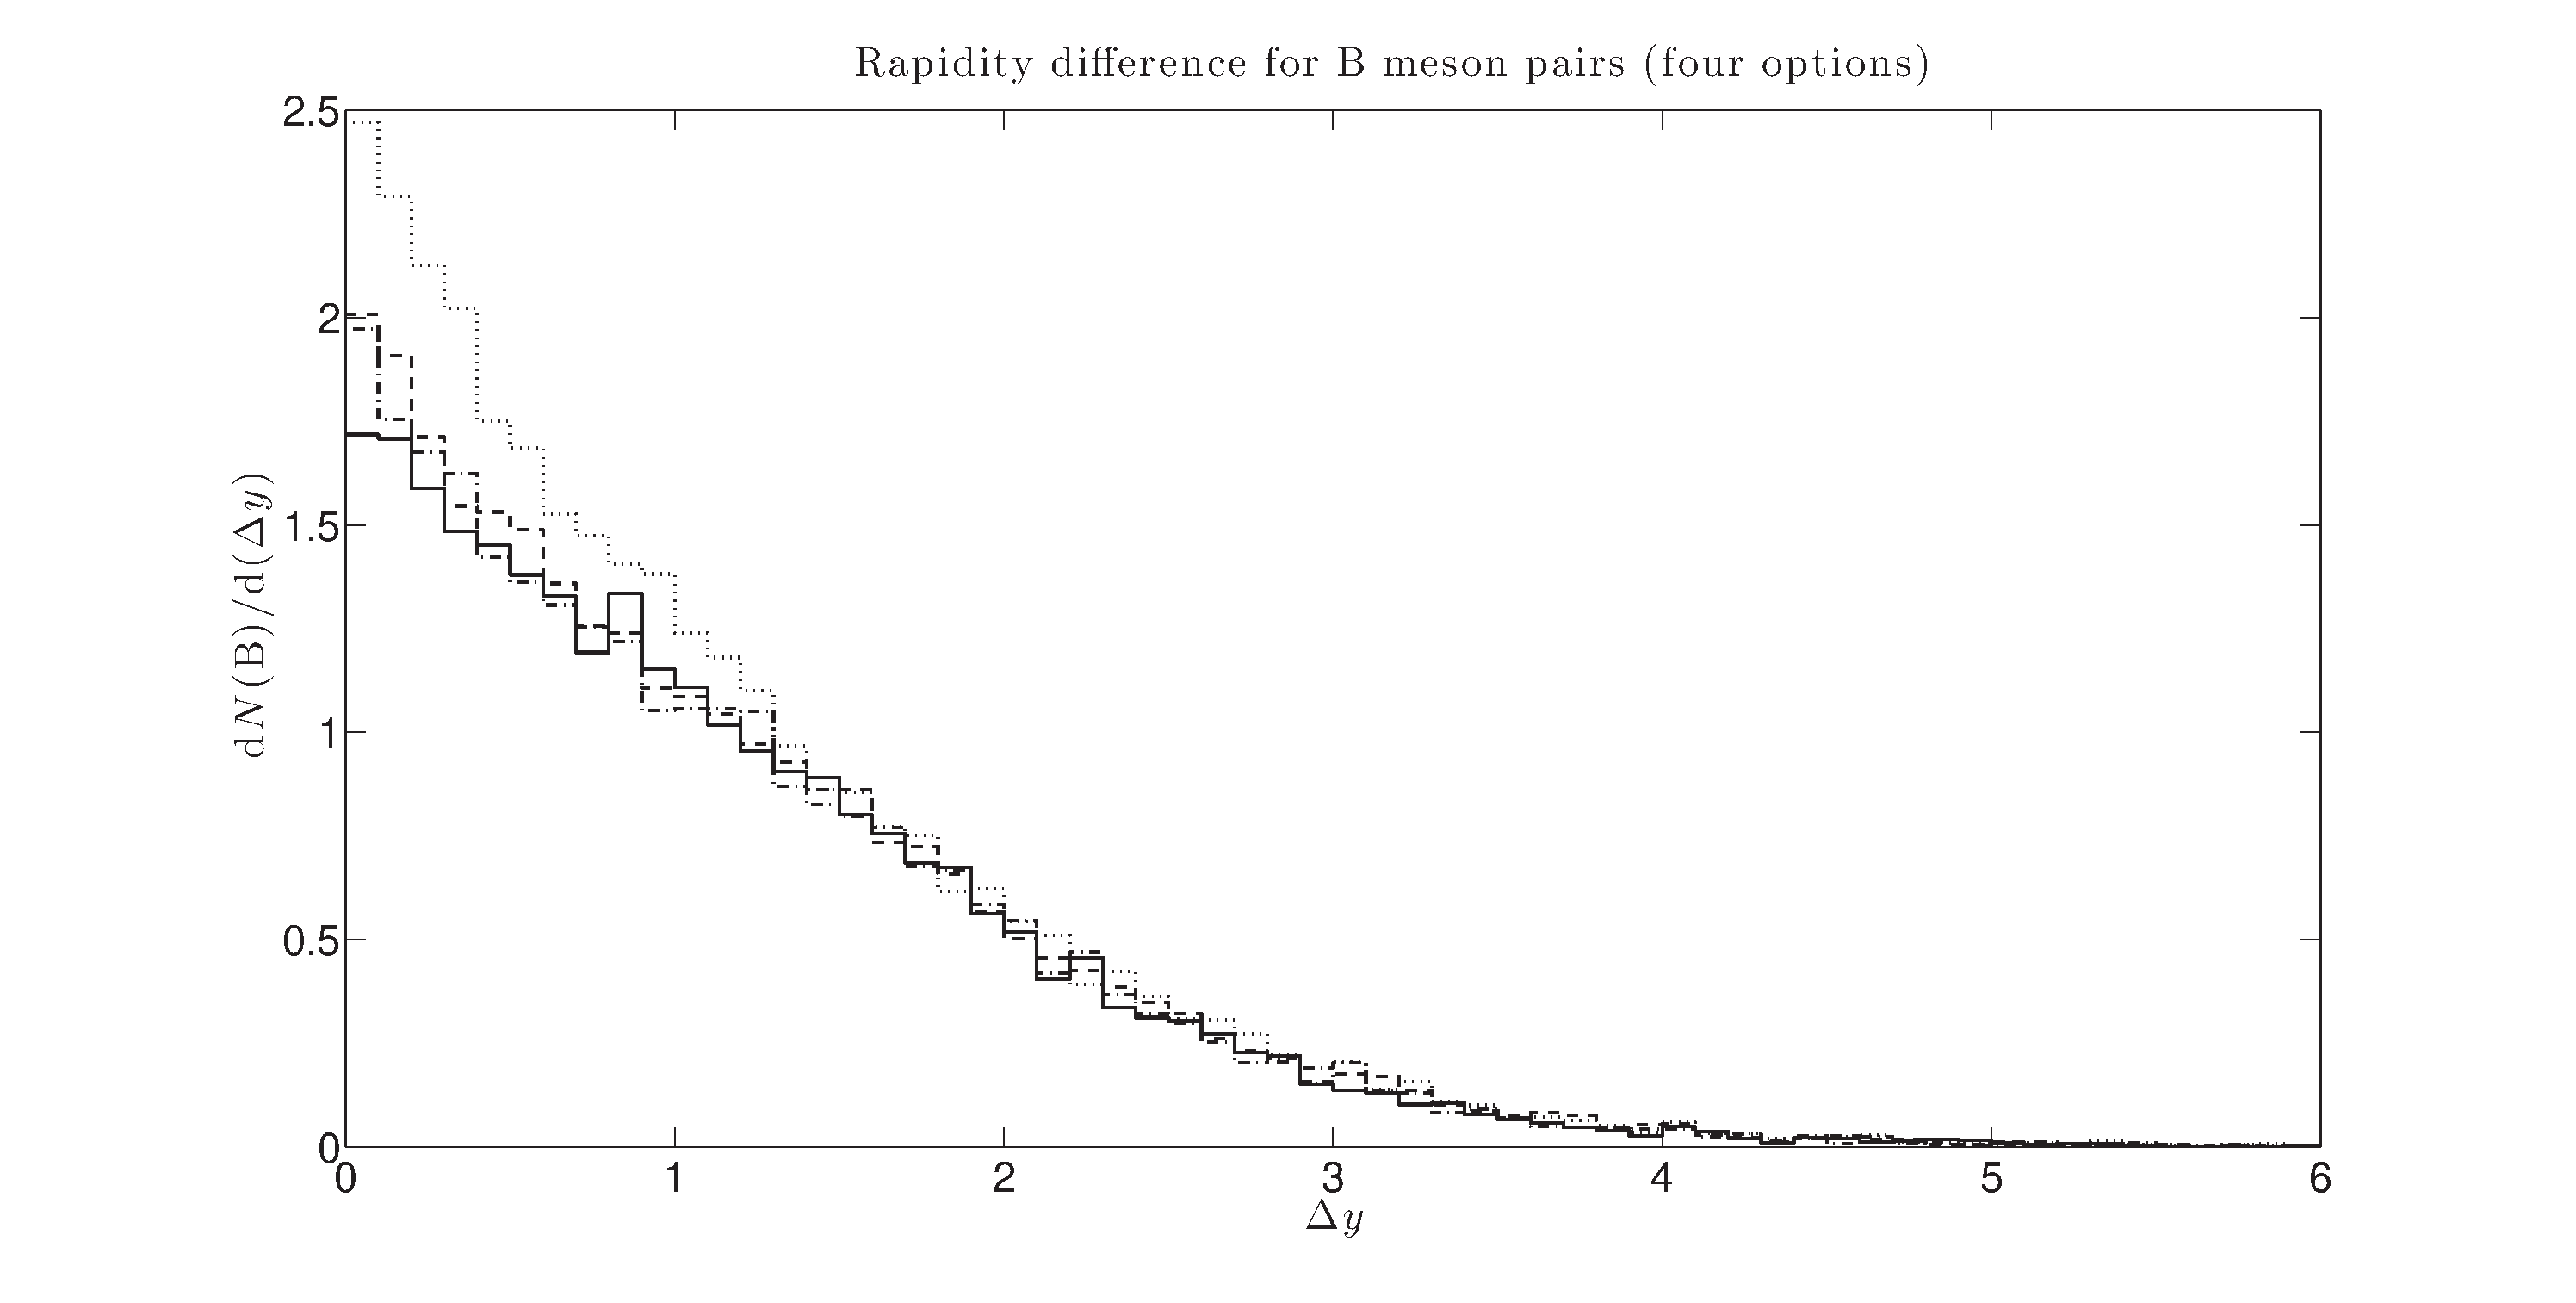
\includegraphics[width=15cm]{BBY4Op}
\label{fig:BBY4Op}
\end{figure}

Diferencias bajas en rapidez significan que las partículas en los pares están cercanas en ``distancia polar'', al mismo tiempo que un $\Delta y$ alto significa una separación polar alta. En principio, los quarks provenientes de PC son producidos con una diferencia de rapidez muy pequeña, pero los efectos cinemáticos de la lluvia de partones abren esta separación y los correspondientes mesones contribuyen significativamente en valores medianos y bajos de $\Delta y$.

La contribución de FE es menos importante que la proveniente de PC. La producción por excitación de sabor cae por debajo de GS únicamente a diferencias de rapidez bajas.

El cambio en las opciones es entonces apreciable a valores bajos de $\Delta y$, mientras que en la región media y en la cola final el comportamiento es similar en las cuatro opciones.

\subsection{Distancias $R$}

La cantidad $R$ contiene información de las dos variables estudiadas anteriormente. En cierto sentido, al dar valores de $\Delta y$ y $\Delta \varphi$ de un par de mesones, se tiene una descripción completa (Lorentz invariante ante boosts en $z$) de la distribución angular del par. En el plano $y - \varphi$ la distancia (también invarinte) $R=\sqrt{(\Delta y)^2 + (\Delta \varphi)^2}$ es útil para agrupar los pares con sus ``vecinos'' angulares. Para definir un \textit{jet de partículas} se usa típicamente la distancia $R$ para agrupar hadrones cercanos.

La figura \ref{fig:BBROp1} muestra el comportamiento de cada fuente, más la producción total de mesones $\B$ para la opción 1.
\begin{figure}[!h]
\centering
\caption[Distancia $R$ de pares de mesones $\B$. Opción por feceto de \textsc{Pythia}.]{ Distancias $R$ de pares de mesones $\B$ usando la opción por defecto de \textsc{Pythia}, incluyendo las cuatro fuentes de producción.}
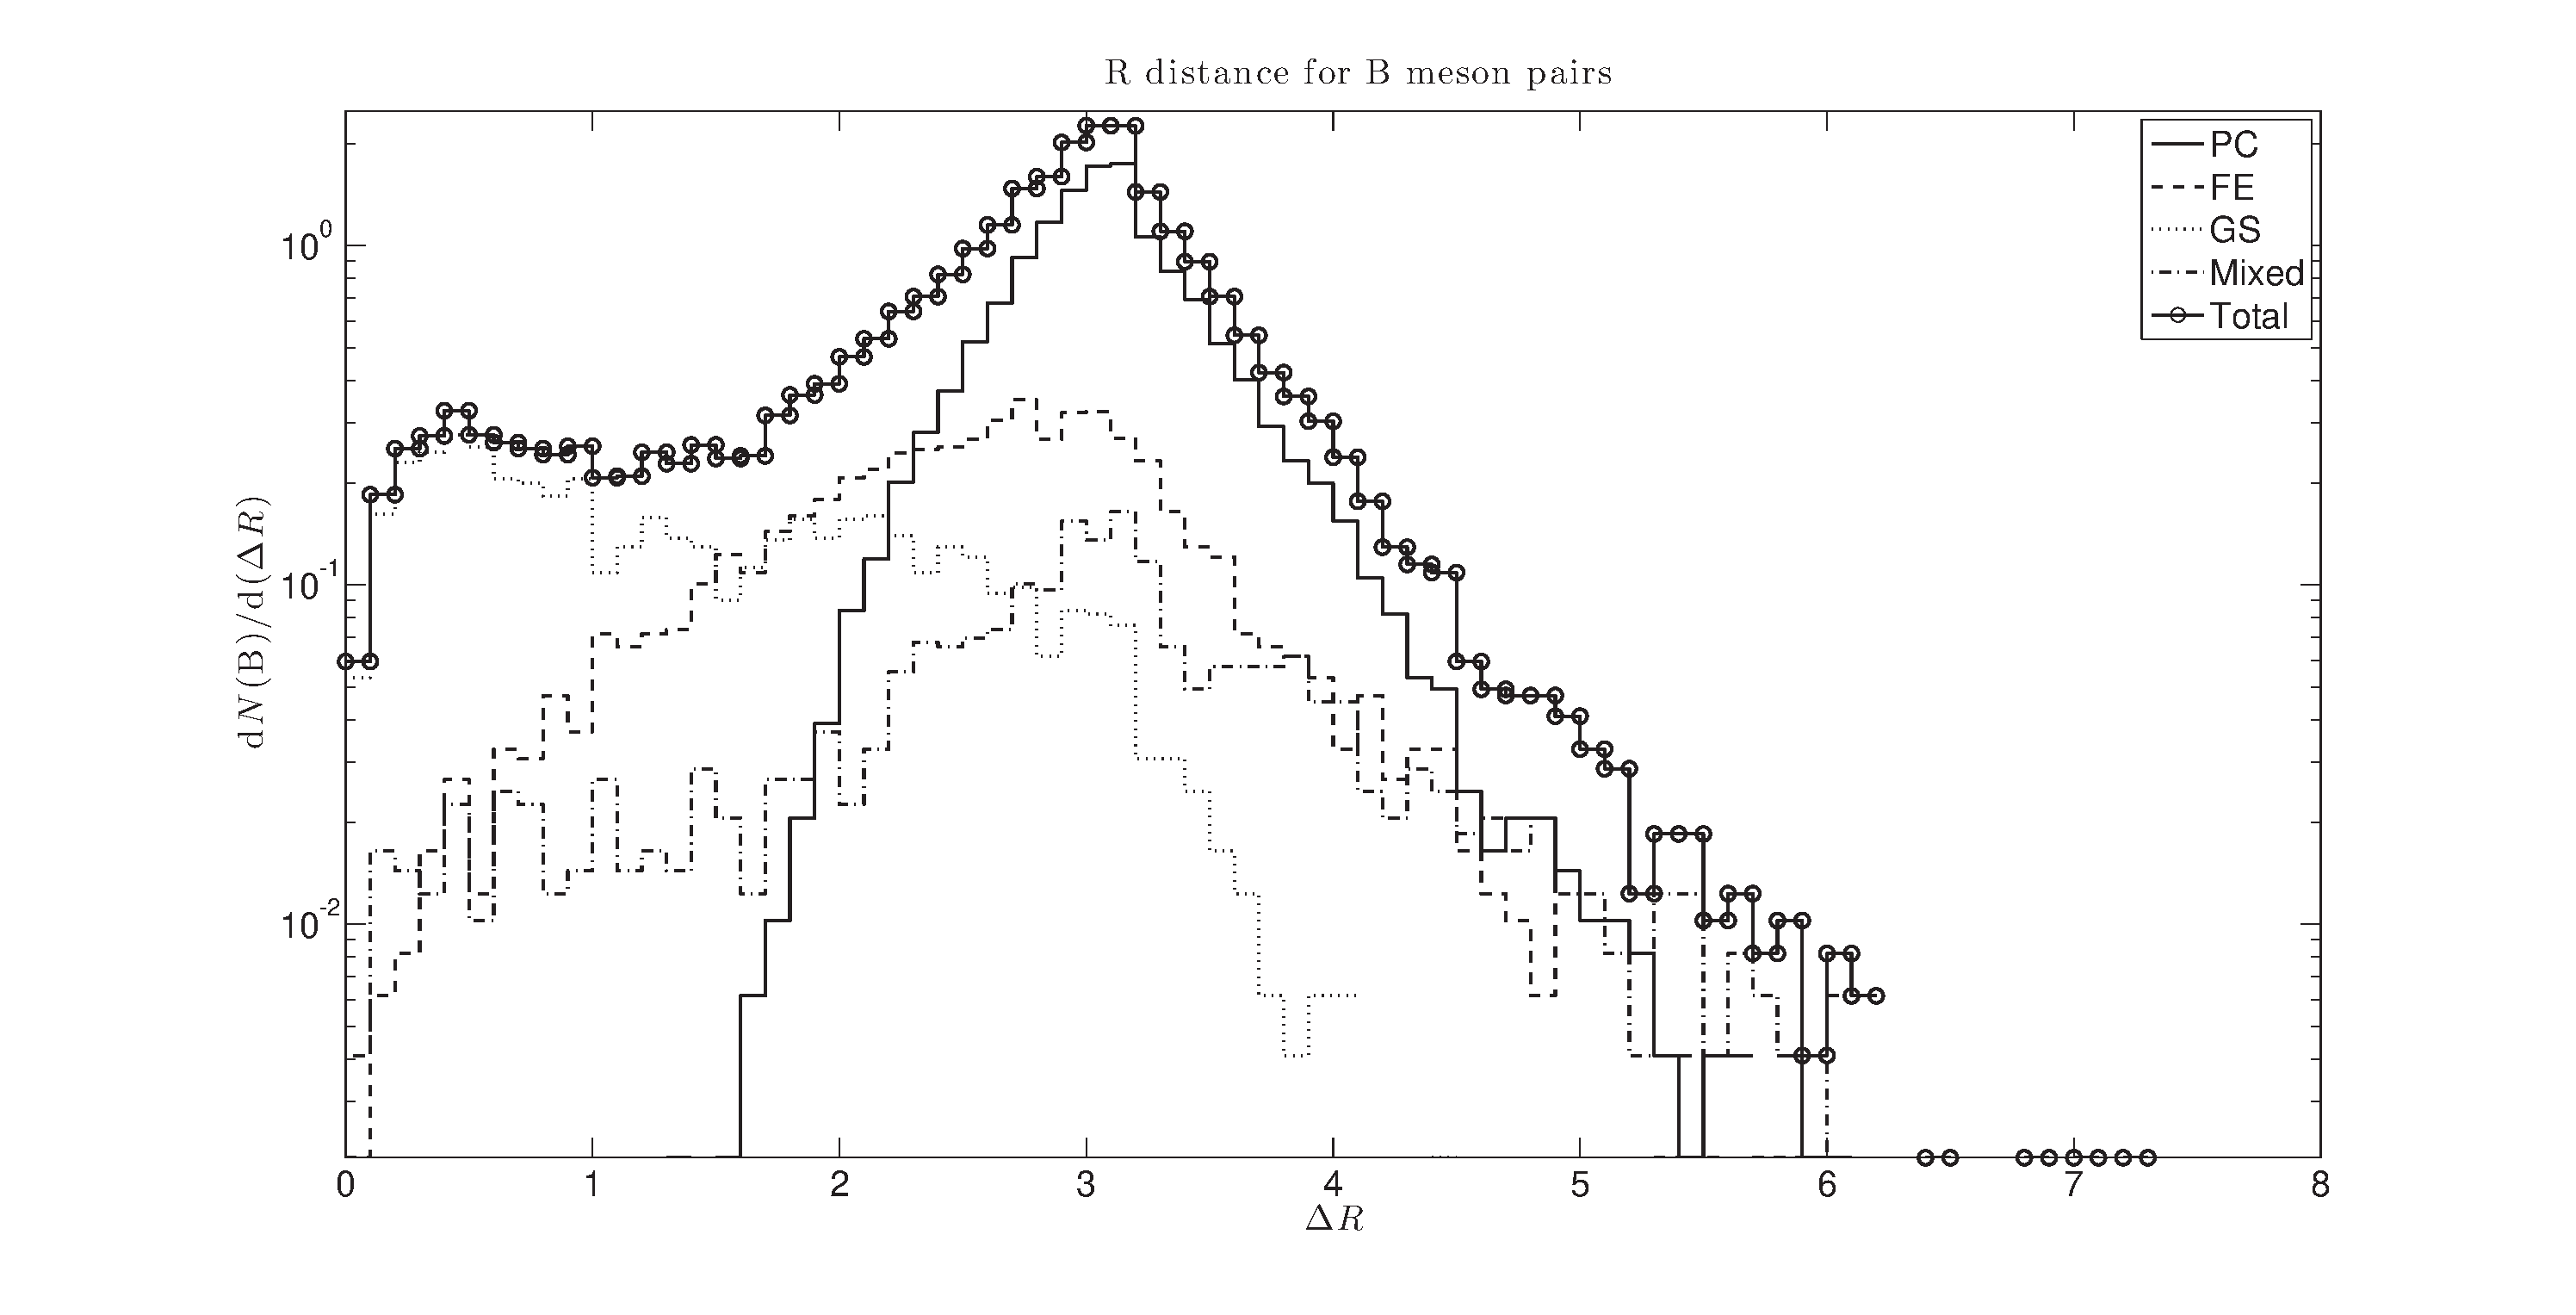
\includegraphics[width=15cm]{BBROp1}
\label{fig:BBROp1}
\end{figure}
Debido a la contribución relevante de PC a ángulos azimutales de abertura grandes, el pico principal de la distancia $R$ es cercano al valor de $\pi$. La excitación de sabor también presenta un crecimiento cerca de ese valor, aunque es menos significativo. Los mesones producidos en GS están usualmente cercanos tanto en $y$ como en $\varphi$, así que los pares clasificados como ramificación de un gluón serán probablemente agrupados en el mismo jet.
\begin{figure}[!h]
\centering
\caption[Distancia $R$ de pares de mesones $\B$. Cuatro opciones de \textsc{Pythia}.]{Distancias $R$ de pares de mesones $\B$ usando las opciones  de \textsc{Pythia}:  1 (sólida), 2 (líneas), 3 (puntos) y 4 (líneas y puntos).}
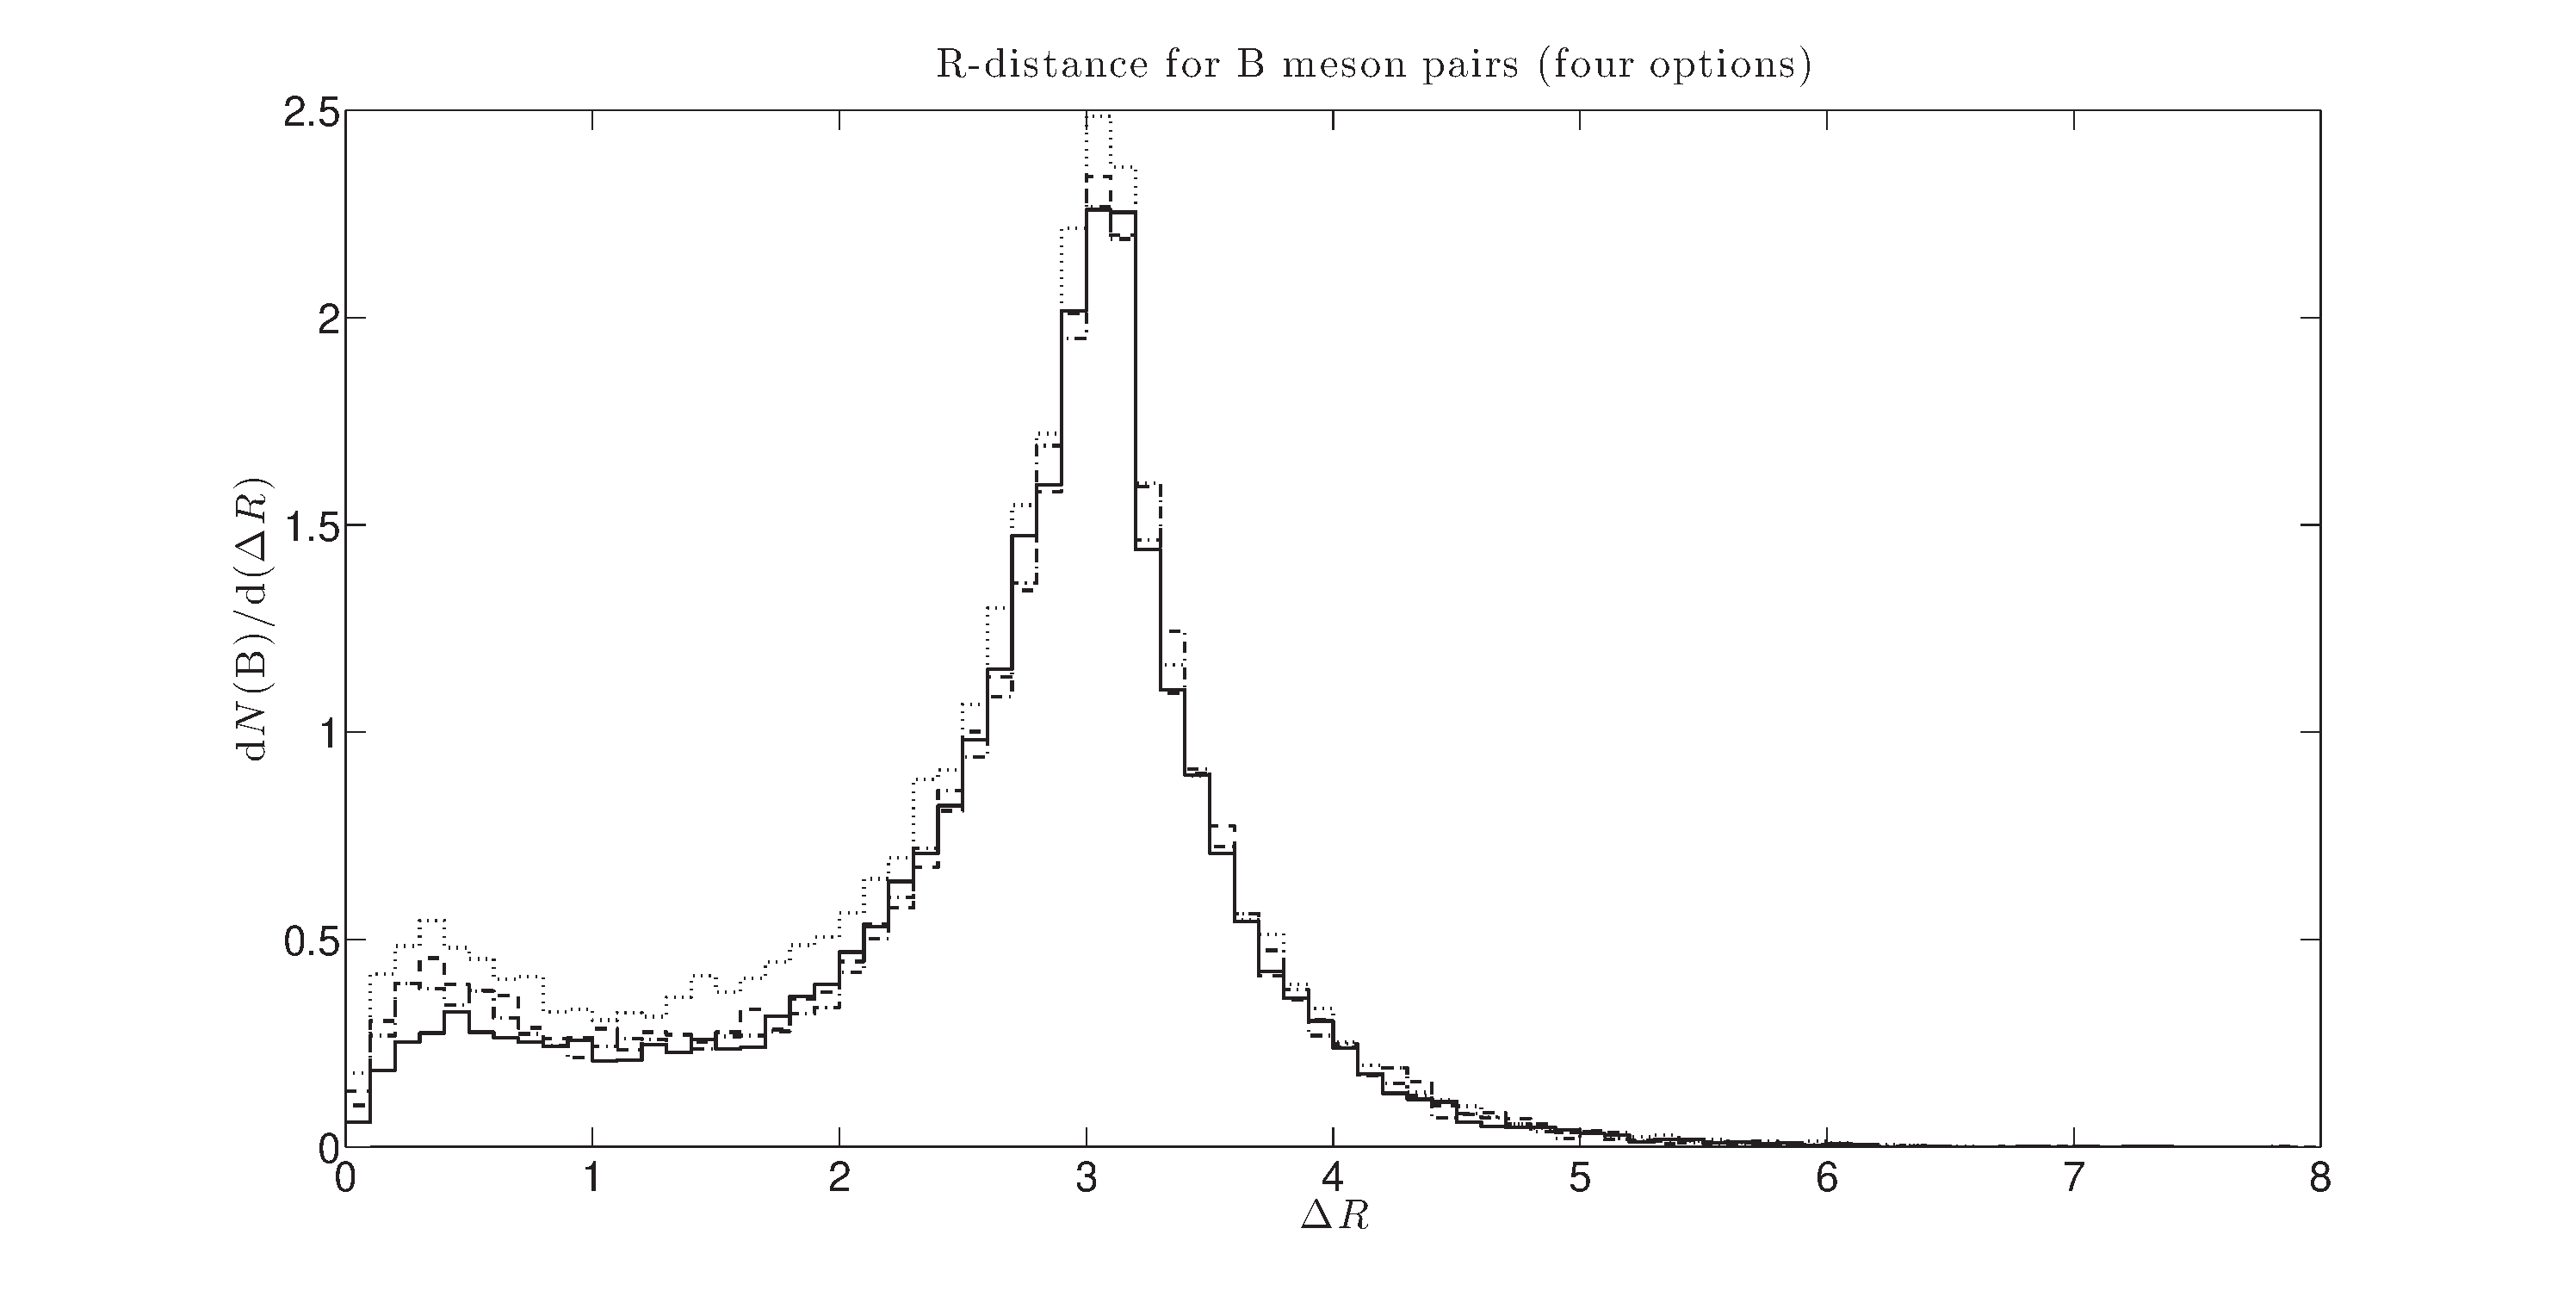
\includegraphics[width=15cm]{BBR4Op}
\label{fig:BBR4Op}
\end{figure}

Debido a que $R$ combina la información de la rapidez relativa y la abertura angular, se espera un aumento respectivo en cada una de las opciones a distancias pequeñas, que se muestra en la figura \ref{fig:BBR4Op}.

Datos experimentales sobre las correlaciones angulares de bottom pueden ser conseguidas en \cite{Khachatryan:2011wq} y \cite{ATLAS:2011ac}. Los análisis hechos ahí están incluidos en un conjunto de rutinas de validación de Rivet \cite{Buckley:2010ar}. La integración entre análisis de \textsc{Pythia} y Rivet, y la producción de datos a partir de esta, fue una maquinaria considerada para este trabajo, aunque no se logró implementar completamente debido a restricciones en el tiempo. El estudio de colisiones hadrónicas puede ser llevado a cabo también para diferentes PDFs, para observar el impacto en los mecanismos de producción y luego comparar con datos experimentales.

Existen también estudios sobre la producción de quarks $\b$ en el Tevatron (colisiones $\p\pbar$ a 2000 GeV), un ejemplo de estos es \cite{vallecorsa}.

%
%\chapter{Conclusiones}
\label{sec:summary}

La tasa de producción $\g_{\b\bbar}$ fue simulada y comparada con resultados experimentales. Los resultados están de acuerdo con la opción por defecto de \textsc{Pythia} y con la opción 4 dentro de los errores experimentales. Curiosamente, el aumento producido por la opción 4 en la región de umbral de masa es casi exactamente cancelado por la supresión a masas altas, lo que conllevó a una tasa cercana a la dada por la opción por defecto. La opción 2 da un resultado dentro de dos desviaciones estándar comparado con los datos experimentales, mientras que la opción 3 no parece reproducir la tasa. Las opciones 5-8, usando $m^2$ como el argumento  del acoplo fuerte, no afecta sensiblemente la tasa (alrededor de 5\% de diferencia para cada opción).

Existe un limitado conjunto de datos disponibles para el estudio de quarks pesados en colisionadores leptónicos. Futuras mediciones de la producción de quarks pesados como función de la masa invariante del par pudiera esclarecer cuál de las opciones es la más adecuada, o la necesidad de una nueva.

El estudio no permite concluir definitivamente sobre la base del espectro de energía de los mesones $\D^{*\pm}$. La opción por defecto muestra una deficiencia a bajas energías que pudiera ser corregida por el aumento dado por las opciones alternativas, particularmente por la opción 3. Sin embargo, todas las opciones presentan un exceso a energías medianas que, de ser corrido a regiones de más bajas energías a través de, por ejemplo, un nuevo modelado del decaimiento $\B\to\D$, pudiera también reconciliar \textsc{Pythia} y los datos experimentales, sin introducir una nueva tasa de producción $\g\to\Q\Qbar$.

Para colisiones protón-protón a energías típicas del LHC, la abertura angular azimutal, las rapideces relativas y las distancias $R$ de pares de mesones $\B$ fueron simuladas. Las contribuciones de los mecanismos de producción a las cantidades mencionadas fueron mostradas. La variación de los observables usando las diferentes opciones de \textsc{Pythia} también fue estudiada y mostrada en los gráficos. Usando cortes inferiores para el momentum transveso para la generación de eventos y para los mesones $\B$ analizados, los eventos seleccionados fueron alrededor de $1.5$ \% de los generados.

Futuros estudios pudieran empezar comparando los resultados simulados de las cuatro opciones con los datos. Existen resultados experimentales y análisis para los experimentos Tevatron y LHC, basados en diferentes mecanismos de reconstrucción de eventos. La dependencia de las correlaciones y tasas de producción  implementando otras PDFs pueden ser también exploradas en este contexto.




\section*{Agradecimientos}

Quisiera agradecer a mi tutor, el profesor Torbjörn Sjöstrand, por su paciente asesoría y correcciones a las versiones iniciales de este trabajo. Las valiosas discusiones con él fueron esenciales para el desarrollo de las ideas presentadas acá. Asimismo, al profesor Fernando Febres Cordero, por desde hace algunos años ya, seguir de cerca mi carrera y la versión de este trabajo en español.

Finalmente, a mis amigos y familiares por su apoyo durante mi estadía en Suecia, país al que le debo, entre otras cosas, mucha física.


\clearpage
\begin{thebibliography}{99}


%\cite{Sjostrand:2006za}
\bibitem{Sjostrand:2006za}
  T.~Sjöstrand, S.~Mrenna and P.~Z.~Skands,
  %``PYTHIA 6.4 Physics and Manual,''
  JHEP {\bf 0605} (2006) 026
  [hep-ph/0603175].
  %%CITATION = HEP-PH/0603175;%%
  %5087 citations counted in INSPIRE as of 28 Apr 2014

%\cite{Sjostrand:2007gs}
\bibitem{Sjostrand:2007gs}
  T.~Sjöstrand, S.~Mrenna and P.~Z.~Skands,
  %``A Brief Introduction to PYTHIA 8.1,''
  Comput.\ Phys.\ Commun.\  {\bf 178} (2008) 852
  [arXiv:0710.3820 [hep-ph]].
  %%CITATION = ARXIV:0710.3820;%%
  %1065 citations counted in INSPIRE as of 28 Apr 2014
  
%\cite{Beringer:1900zz}
\bibitem{Beringer:1900zz}
  J.~Beringer {\it et al.}  [Particle Data Group Collaboration],
  %``Review of Particle Physics (RPP),''
  Phys.\ Rev.\ D {\bf 86} (2012) 010001.
  %%CITATION = PHRVA,D86,010001;%%
  %3768 citations counted in INSPIRE as of 29 Apr 2014  

%\cite{Kane:1993}
\bibitem{Kane:1993}
 G.~Kane,
 ``Modern elementary particle physics: the fundamental particles and forces?,''
 Perseus publishing (1993).
 %%CITATION = HPACA,25,417;%%

%\cite{Peskin:1995} 
\bibitem{Peskin:1995}
  M.~E.~Peskin and D.~V.~Schroeder,
  ``An Introduction To Quantum Field Theory,''
%\href{http://www.slac.stanford.edu/spires/find/hep/www?irn=3485960}{SPIRES entry}
{\it  Reading, USA: Addison-Wesley (1995) 842 p}.

%\cite{Sjostrand:2009ad}
\bibitem{Sjostrand:2009ad}
  T.~Sjöstrand,
  %``Monte Carlo Tools,''
  arXiv:0911.5286 [hep-ph].
  %%CITATION = ARXIV:0911.5286;%%
  %11 citations counted in INSPIRE as of 28 Apr 2014

%\cite{Boos:2001cv}
\bibitem{Boos:2001cv}
  E.~Boos, M.~Dobbs, W.~Giele, I.~Hinchliffe, J.~Huston, V.~Ilyin, J.~Kanzaki and K.~Kato {\it et al.},
  %``Generic user process interface for event generators,''
  hep-ph/0109068.
  %%CITATION = HEP-PH/0109068;%%
  %175 citations counted in INSPIRE as of 21 Jun 2014

% The next five articles correspond to the measurement of the g_{bb} rate.
%\cite{Abreu:1997nf} \cite{Barate:1998vs} \cite{Abe:1999qg} \cite{Abreu:1999qh} \cite{Abbiendi:2000zt}

% \cite{Abreu:1997nf}
\bibitem{Abreu:1997nf}
  P.~Abreu {\it et al.}  [DELPHI Collaboration],
  %``Measurement of the multiplicity of gluons splitting to bottom quark pairs in hadronic Z0 decays,''
  Phys.\ Lett.\ B {\bf 405} (1997) 202.
  %%CITATION = PHLTA,B405,202;%%
  %45 citations counted in INSPIRE as of 15 May 2014
  
%\cite{Barate:1998vs}
\bibitem{Barate:1998vs}
  R.~Barate {\it et al.}  [ALEPH Collaboration],
  %``A Measurement of the gluon splitting rate into b anti-b pairs in hadronic Z decays,''
  Phys.\ Lett.\ B {\bf 434} (1998) 437.
  %%CITATION = PHLTA,B434,437;%%
  %42 citations counted in INSPIRE as of 15 May 2014
  
%\cite{Abe:1999qg}
\bibitem{Abe:1999qg}
  K.~Abe {\it et al.}  [SLD Collaboration],
  %``Measurement of the probability for gluon splitting into b anti-b in Z0 decays,''
  hep-ex/9908028.
  %%CITATION = HEP-EX/9908028;%%
  %8 citations counted in INSPIRE as of 15 May 2014
  
%\cite{Abreu:1999qh}
\bibitem{Abreu:1999qh}
  P.~Abreu {\it et al.}  [DELPHI Collaboration],
  %``Measurement of the rate of b anti-b b anti-b events in hadronic Z decays and the extraction of the gluon splitting into b anti-b,''
  Phys.\ Lett.\ B {\bf 462} (1999) 425.
  %%CITATION = PHLTA,B462,425;%%
  %27 citations counted in INSPIRE as of 15 May 2014

%\cite{Abbiendi:2000zt}
\bibitem{Abbiendi:2000zt}
  G.~Abbiendi {\it et al.}  [OPAL Collaboration],
  %``Production rates of b anti-b quark pairs from gluons and b anti-b b anti-b events in hadronic Z0 decays,''
  Eur.\ Phys.\ J.\ C {\bf 18} (2001) 447
  [hep-ex/0010029].
  %%CITATION = HEP-EX/0010029;%%
  %16 citations counted in INSPIRE as of 19 May 2014

%\cite{Barate:1999bg}
\bibitem{Barate:1999bg}
  R.~Barate {\it et al.}  [ALEPH Collaboration],
  %``Study of charm production in Z decays,''
  Eur.\ Phys.\ J.\ C {\bf 16} (2000) 597
  [hep-ex/9909032].
  %%CITATION = HEP-EX/9909032;%%
  %123 citations counted in INSPIRE as of 11 May 2014
  
%\cite{Norrbin:2000zc}
\bibitem{Norrbin:2000zc}
  E.~Norrbin and T.~Sjöstrand,
  %``Production and hadronization of heavy quarks,''
  Eur.\ Phys.\ J.\ C {\bf 17} (2000) 137
  [hep-ph/0005110].
  %%CITATION = HEP-PH/0005110;%%
  %113 citations counted in INSPIRE as of 12 May 2014

%\cite{Khachatryan:2011wq} \cite{ATLAS:2011ac}
\bibitem{Khachatryan:2011wq}
  V.~Khachatryan {\it et al.}  [CMS Collaboration],
  %``Measurement of $B\bar{B}$ Angular Correlations based on Secondary Vertex Reconstruction at $\sqrt{s}=7$ TeV,''
  JHEP {\bf 1103} (2011) 136
  [arXiv:1102.3194 [hep-ex]].
  %%CITATION = ARXIV:1102.3194;%%
  %50 citations counted in INSPIRE as of 26 May 2014

%\cite{ATLAS:2011ac}
\bibitem{ATLAS:2011ac}
  G.~Aad {\it et al.}  [ATLAS Collaboration],
  %``Measurement of the inclusive and dijet cross-sections of $b^-$ jets in $pp$ collisions at $\sqrt{s}=7$ TeV with the ATLAS detector,''
  Eur.\ Phys.\ J.\ C {\bf 71} (2011) 1846
  [arXiv:1109.6833 [hep-ex]].
  %%CITATION = ARXIV:1109.6833;%%
  %41 citations counted in INSPIRE as of 26 May 2014

%\cite{Buckley:2010ar}
\bibitem{Buckley:2010ar}
  A.~Buckley, J.~Butterworth, L.~Lonnblad, D.~Grellscheid, H.~Hoeth, J.~Monk, H.~Schulz and F.~Siegert,
  %``Rivet user manual,''
  Comput.\ Phys.\ Commun.\  {\bf 184} (2013) 2803
  [arXiv:1003.0694 [hep-ph]].
  %%CITATION = ARXIV:1003.0694;%%
  %137 citations counted in INSPIRE as of 21 Jun 2014

%\cite{vallecorsa}
\bibitem{vallecorsa}
  S. Vallecorsa,
  ``Measurement of the $\b\bbar$ di-jet cross section at CDF,''
  Univ. of Geneva Thesis (2007) 3916.

\end{thebibliography}

%\includegraphics[width=8cm]{Draco_cmd.ps}

\end{onehalfspace}

\end{document}
